% Author: Simon-Pierre Boucher — contact@spboucher.ai
%
% ============================================================================
% UQO Working Paper No. 3
% Hedonic Housing Price Models for the United States: A Multi-Method
% Comparison of Parametric, Quantile, and Machine Learning Approaches
% ============================================================================
\documentclass[12pt,letterpaper]{article}

% --- Encoding & Language ---
\usepackage[utf8]{inputenc}
\usepackage[T1]{fontenc}
\usepackage[english]{babel}

% --- Page Layout ---
\usepackage[letterpaper, margin=1in, headheight=15pt]{geometry}
\usepackage{setspace}
\onehalfspacing
\setlength{\parindent}{1.5em}
\setlength{\parskip}{0pt}

% --- Typography ---
\usepackage{newtxtext,newtxmath}
\usepackage{amsmath,amsfonts}
\let\Bbbk\relax
\usepackage{amssymb}
\usepackage{mathtools}
\usepackage{microtype}

% --- Tables ---
\usepackage{booktabs}
\usepackage{threeparttable}
\usepackage{tabularx}
\usepackage{array}
\usepackage{multirow}
\usepackage{longtable}
\usepackage{adjustbox}
\usepackage{siunitx}
\usepackage{dcolumn}

% --- Figures ---
\usepackage{graphicx}
\graphicspath{{./}{../}}  % figures live in ../figures/, logo in ./
\usepackage[
  font       = small,
  labelfont  = bf,
  labelsep   = period,
  skip       = 8pt,
  justification = justified,
  singlelinecheck = false
]{caption}
\usepackage{subcaption}
\usepackage{float}
\usepackage{pdflscape}

% --- Colors & Links ---
\usepackage[dvipsnames]{xcolor}
\definecolor{linkblue}{RGB}{0,51,102}
\usepackage[bookmarks, bookmarksnumbered]{hyperref}
\hypersetup{
  colorlinks  = true,
  linkcolor   = NavyBlue,
  citecolor   = NavyBlue,
  urlcolor    = NavyBlue,
  pdftitle    = {Hedonic Housing Price Models for the United States: A Multi-Method Comparison of Parametric, Quantile, and Machine Learning Approaches},
  pdfauthor   = {Simon-Pierre Boucher}
}

% --- Bibliography ---
\usepackage[round, authoryear, comma]{natbib}
\setcitestyle{aysep={,}}
\bibliographystyle{apalike}

% --- Headers & Footers ---
\usepackage{fancyhdr}
\pagestyle{fancy}
\fancyhf{}
\fancyhead[L]{\small\itshape Hedonic Housing Price Models for the United States}
\fancyhead[R]{\small\thepage}
\renewcommand{\headrulewidth}{0.4pt}
\renewcommand{\footrulewidth}{0pt}
\fancypagestyle{plain}{%
  \fancyhf{}
  \fancyfoot[C]{\small\thepage}
  \renewcommand{\headrulewidth}{0pt}
}

% --- Section Formatting ---
\usepackage{titlesec}
\titleformat{\section}{\large\bfseries}{\thesection.}{0.5em}{}
\titleformat{\subsection}{\normalsize\bfseries}{\thesubsection.}{0.5em}{}
\titleformat{\subsubsection}{\normalsize\itshape}{\thesubsubsection.}{0.5em}{}

% --- Appendix Support ---
\usepackage[toc, page]{appendix}
\usepackage{enumitem}
\usepackage{etoolbox}
\usepackage[hang,flushmargin]{footmisc}

% --- Custom Column Types ---
\newcolumntype{R}[1]{>{\raggedleft\arraybackslash}p{#1}}
\newcolumntype{L}[1]{>{\raggedright\arraybackslash}p{#1}}
\newcolumntype{C}[1]{>{\centering\arraybackslash}p{#1}}
\newcolumntype{d}[1]{D{.}{.}{#1}}

% --- Custom Commands ---
\newcommand{\sym}[1]{\ensuremath{^{#1}}}
\newcommand{\stmark}[1]{\rlap{\textsuperscript{#1}}}
\DeclareMathOperator*{\plim}{plim}
\newcommand{\E}{\mathbb{E}}
\newcommand{\Var}{\mathrm{Var}}
\newcommand{\Cov}{\mathrm{Cov}}
\newcommand{\Corr}{\mathrm{Corr}}
\newcommand{\se}{\mathrm{s.e.}}
\newcommand{\tr}{\mathrm{tr}}
\newcommand{\rank}{\mathrm{rank}}
\newcommand{\diag}{\mathrm{diag}}
\newcommand{\R}{\mathbb{R}}
\newcommand{\N}{\mathbb{N}}
\newcommand{\eps}{\varepsilon}
\newcommand{\bfbeta}{\boldsymbol{\beta}}
\newcommand{\bfgamma}{\boldsymbol{\gamma}}
\newcommand{\bfalpha}{\boldsymbol{\alpha}}
\newcommand{\bfdelta}{\boldsymbol{\delta}}
\newcommand{\bftheta}{\boldsymbol{\theta}}
\newcommand{\bfSigma}{\boldsymbol{\Sigma}}
\newcommand{\bfOmega}{\boldsymbol{\Omega}}
\newcommand{\bfX}{\mathbf{X}}
\newcommand{\bfY}{\mathbf{Y}}
\newcommand{\bfy}{\mathbf{y}}
\newcommand{\bfe}{\mathbf{e}}
\newcommand{\bfs}{\mathbf{s}}
\newcommand{\iid}{\overset{\mathrm{iid}}{\sim}}
\newcommand{\pto}{\overset{p}{\to}}
\newcommand{\dto}{\overset{d}{\to}}
\newcommand{\ols}{\mathrm{OLS}}
\newcommand{\iv}{\mathrm{IV}}
\newcommand{\gmm}{\mathrm{GMM}}
\newcommand{\mle}{\mathrm{MLE}}
\newcommand{\pval}{\textit{p}-value}
\newcommand{\tstat}{\textit{t}-statistic}
\newcommand{\fstat}{\textit{F}-statistic}
\newcommand{\tablenote}[1]{\begin{minipage}{\linewidth}\footnotesize #1\end{minipage}}
\newcommand{\signote}{*** $p < 0.001$; ** $p < 0.01$; * $p < 0.05$.}

% ============================================================================
% METADATA
% ============================================================================
\newcommand{\WPnumber}{3}
\newcommand{\WPtitle}{Hedonic Housing Price Models for the United States: A Multi-Method Comparison of Parametric, Quantile, and Machine Learning Approaches}
\newcommand{\WPsubtitle}{}
\newcommand{\WPdate}{May 2026}
\newcommand{\WPversion}{1.0}
\newcommand{\WPabstract}{%
This paper compares econometric and machine-learning approaches to hedonic housing valuation using 788,842 active Zillow listings across all 50 U.S.\ states and the District of Columbia. A semi-log OLS model with 62 regressors ($R^2 = 0.634$) provides interpretable listing-price gradients; adding ZIP3 fixed effects raises $R^2$ to 0.725, and Moran's $I = 0.27$ confirms strong residual spatial autocorrelation. Quantile regression reveals distributional heterogeneity, with inter-quantile Wald tests rejecting coefficient equality between $\tau = 0.10$ and $\tau = 0.90$ for 11 of 13 key variables. XGBoost achieves $R^2 = 0.833$ under random validation but only 0.425 under state-level geographic holdout; ablation analysis traces the predictive gain primarily to neighborhood-quality features ($+17.6$ pp) and shows that removing geographic features \emph{improves} geographic holdout $R^2$ to 0.519, revealing spatial overfitting. SHAP importance rankings are stable across models (Spearman $\rho > 0.89$). Robustness checks confirm that the lot-size gradient triples when imputed observations are dropped, while other coefficients remain stable under winsorization and subsampling. Throughout, estimates are interpreted as conditional associations in listing prices, not causal willingness-to-pay parameters.%
}
\newcommand{\WPkeywords}{hedonic pricing, housing markets, quantile regression, XGBoost, SHAP, spatial autocorrelation, geographic validation}
\newcommand{\WPjel}{R31, C21, C45, C52}

% --- Author ---
\newcommand{\WPauthor}{Simon-Pierre Boucher}
\newcommand{\WPaffiliation}{%
  D\'epartement des sciences administratives\\
  Universit\'e du Qu\'ebec en Outaouais%
}
\newcommand{\WPemail}{simon-pierre.boucher@uqo.ca}
\newcommand{\WPaddress}{%
  Gatineau -- Pavillon Alexandre-Tach\'e\\
  283, boulevard Alexandre-Tach\'e\\
  Gatineau, Qu\'ebec, Canada J9A 1L8%
}

% ============================================================================
% DOCUMENT
% ============================================================================
\begin{document}

% --- Title Page ---
% Author: Simon-Pierre Boucher — contact@spboucher.ai
%
% ============================================================================
% Title Page
% ============================================================================
\thispagestyle{empty}

\begin{center}

% --- Logo ---

\includegraphics[width=3.5cm]{uq_logo.jpg}

\vspace{0.6cm}

{\footnotesize\textsc{Universit\'e du Qu\'ebec en Outaouais}}\\[0.15cm]
{\footnotesize\textsc{D\'epartement des sciences administratives}}

\vspace{0.8cm}

{\footnotesize\textsc{Working Paper No.~\WPnumber}}

\vspace{1.2cm}

% --- Title ---
{\LARGE\bfseries \WPtitle\par}

\ifx\WPsubtitle\empty\else
  \vspace{0.3cm}
  {\large\itshape \WPsubtitle\par}
\fi

\vspace{1.2cm}

% --- Author ---
{\large \WPauthor\footnotemark[1]}\\[0.3cm]
{\normalsize\itshape \WPaffiliation}

\footnotetext[1]{D\'epartement des sciences administratives, Universit\'e du Qu\'ebec en Outaouais (UQO), 283 boulevard Alexandre-Tach\'e, Gatineau, QC J9A 1L8, Canada. Email: \href{mailto:\WPemail}{\WPemail}. All errors are my own.}

\vspace{0.8cm}

% --- Date & Version ---
{\normalsize First draft: May 2026}\\[0.1cm]
{\normalsize This version: August 5, 2026}\\[0.1cm]
{\small\itshape Version~\WPversion}

\end{center}

\vfill

\newpage

% ============================================================================
% Abstract Page
% ============================================================================
\thispagestyle{empty}

\vspace*{1cm}

\noindent\rule{\textwidth}{0.4pt}
\vspace{0.3cm}

\noindent\textbf{Abstract}

\vspace{0.15cm}

\noindent\WPabstract

\vspace{0.4cm}

\noindent\textbf{Keywords:} \WPkeywords

\vspace{0.15cm}

\noindent\textbf{JEL Classification:} \WPjel

\vspace{0.3cm}
\noindent\rule{\textwidth}{0.4pt}

\newpage


% --- Main Body ---
% Author: Simon-Pierre Boucher — contact@spboucher.ai
%
% ═══════════════════════════════════════════════════════════════════════
% 1. INTRODUCTION
% ═══════════════════════════════════════════════════════════════════════
\section{Introduction}
\label{sec:introduction}

Housing is the dominant asset in the typical American household's portfolio, the
collateral underpinning the largest class of household debt, and a central object
of study in urban economics, household finance, and public policy. How housing
attributes map into prices matters far beyond academia: property-tax assessment,
mortgage underwriting, and the automated valuation models (AVMs) that increasingly
mediate transactions all rest on some version of that mapping. The hedonic pricing
framework---formalized by \citet{rosen1974hedonic} on the consumer-theoretic
foundations of \citet{lancaster1966new}, with empirical roots stretching back to
\citet{waugh1928quality} and \citet{court1939hedonic}---provides the canonical
approach: decompose observed prices into the implicit valuations of constituent
characteristics. Yet after five decades of applied hedonic research, three
methodological tensions remain unresolved, and the arrival of machine-learning
valuation has sharpened rather than settled them.

First, the standard OLS hedonic model imposes a (log-)linear relationship between
attributes and prices, an assumption chosen largely for robustness under attribute
omission \citep{cropper1988choice} but one that may poorly approximate the
non-linear, interactive structure of housing markets. Second, by estimating
conditional mean effects, OLS constrains implicit prices to be constant across the
price distribution---a restriction the quantile-regression literature has shown to
be empirically untenable \citep{zietz2008determinants, mcmillen2008changes,
liao2012hedonic}. Third, while gradient-boosted models deliver large predictive
gains in property valuation \citep{bourassa2010predicting, kok2017big}, their
black-box character limits adoption where economic interpretation matters
\citep{mullainathan2017machine, athey2019machine}---and, as this paper documents,
their headline accuracy can be a partial illusion created by the way they are
evaluated.

This paper confronts the three tensions on a single dataset of 788,842 active
Zillow listings covering all 50 U.S. states and the District of Columbia, with 62
regressors spanning structural attributes, lot characteristics, amenities,
neighborhood quality, market status, and six interaction terms. We estimate three
families of models, each answering a distinct question:
\begin{enumerate}[nosep]
    \item \textbf{Semi-log OLS} with HC3 robust standard errors---and progressively
    finer geographic fixed effects---for interpretable conditional mean
    associations;
    \item \textbf{Quantile regression} at five quantiles, with formal
    inter-quantile Wald tests, for distribution-specific listing-price gradients;
    \item \textbf{Gradient-boosted ensembles} (XGBoost, LightGBM) with SHAP-based
    interpretation \citep{lundberg2017unified} for non-linear prediction.
\end{enumerate}

The core methodological contribution is a systematic examination of
\textbf{spatial leakage} in hedonic model evaluation. Housing data are spatially
dependent: nearby properties share unobserved local price determinants
\citep{dubin1998spatial, basu1998analysis}. Standard random train-test splits
therefore allow information to leak from training to test sets through spatial
proximity, inflating out-of-sample performance---a phenomenon documented in
ecology and geostatistics \citep{roberts2017cross, ploton2020spatial,
meyer2021predicting} but rarely confronted in housing economics. We quantify its
consequences through three complementary designs: (i) a \emph{geographic holdout}
in which ten entire states (438,315 listings) are withheld from training; (ii) a
six-stage \emph{ablation cascade} that traces the XGBoost predictive gain to
specific feature groups under both validation schemes and reveals that region
dummies actively \emph{harm} geographic generalization; and (iii) a
\emph{coordinate experiment} in which adding raw latitude and longitude boosts
random-split $R^2$ by 3.7 percentage points while \emph{reducing} geographic
holdout $R^2$ by 5.5 percentage points. Together these designs show that the gap
between random and geographic validation is not a matter of degree: the two
protocols measure qualitatively different model capabilities---interpolation
within observed markets versus extrapolation to new ones---and they rank feature
sets differently.

Our contribution is methodological and empirical, not causal. Following the
identification literature \citep{bartik1987estimation, ekeland2004identification,
kuminoff2013new, bishop2020best}, we interpret all estimates as conditional
associations in \emph{listing} prices---capitalization gradients in asking
prices---rather than structural willingness-to-pay parameters, and we engage the
listing-price microstructure literature \citep{horowitz1992role, genesove2001loss,
han2016role} when drawing that distinction. Within that discipline, the paper
makes four contributions:

\begin{enumerate}[nosep]
    \item \textbf{Geographic granularity in OLS.} Progressively finer spatial
    fixed effects (region $\rightarrow$ state $\rightarrow$ ZIP3) raise $R^2$ from
    0.634 to 0.725, providing national-scale, prediction-oriented evidence for the
    specification advice of \citet{kuminoff2010which}; residual Moran's $I$ of
    0.27 shows that even ZIP3 controls leave substantial spatial structure
    unabsorbed.
    \item \textbf{Formal distributional heterogeneity.} Inter-quantile Wald tests
    reject coefficient equality between the 10th and 90th conditional percentiles
    for 11 of 13 key attributes; the pattern (garage and living-area gradients
    concentrated at the bottom of the distribution, pool and lot-size gradients at
    the top) is stable across ten independent subsamples.
    \item \textbf{Anatomy of the ML advantage.} XGBoost's $R^2 = 0.833$ under
    random validation falls to 0.425--0.547 under state-level holdout; removing
    all geographic features \emph{improves} geographic holdout $R^2$ to 0.519.
    The ablation traces the random-validation gain primarily to
    neighborhood-quality variables ($+17.6$ pp) and shows their contribution
    largely fails to transfer across states.
    \item \textbf{Cross-model stability of SHAP.} Importance rankings correlate at
    $\rho = 0.89$--$0.99$ across XGBoost, LightGBM, and random forests, supporting
    SHAP as a description of predictive structure while our framing---informed by
    the explainability debate \citep{rudin2019stop}---keeps it distinct from
    Rosen's implicit prices.
\end{enumerate}

For practitioners, the message is direct: in AVM deployment contexts that require
generalization to unfamiliar markets, validation design is not a technicality but
the difference between a model that appears excellent and one that actually
transfers; and geographic features, however helpful in-sample, can be
counterproductive out-of-market \citep{steurer2021metrics}. For researchers, the
results argue that random-split accuracy comparisons between ML and hedonic
models---now common in the literature---systematically overstate the ML advantage
whenever the deployment question involves new locations.

The remainder of the paper is organized as follows.
Section~\ref{sec:literature} situates the study in the hedonic, quantile,
machine-learning, and spatial-validation literatures.
Section~\ref{sec:data} describes the data, sample construction, variable coding,
and the listing-price caveat. Section~\ref{sec:methodology} presents the
econometric and machine-learning methodology, the three validation designs, and
the interpretation framework. Section~\ref{sec:results} reports estimation
results across the three model families. Section~\ref{sec:robustness} presents
imputation, winsorization, and subsample-stability checks.
Section~\ref{sec:discussion} interprets the findings against the literature,
Section~\ref{sec:limitations} enumerates limitations, and
Section~\ref{sec:conclusion} concludes.

% Author: Simon-Pierre Boucher — contact@spboucher.ai
%
% ═══════════════════════════════════════════════════════════════════════
% 2. LITERATURE REVIEW
% ═══════════════════════════════════════════════════════════════════════
\section{Literature Review}
\label{sec:literature}

This paper sits at the intersection of four literatures: the hedonic pricing
tradition in housing economics, the econometrics of distributional heterogeneity,
the rapidly growing machine-learning strand of property valuation, and the
methodological literature on validating predictive models under spatial dependence.
We review each in turn, emphasizing in every case how it bears on the design choices
of this study and where the gap addressed by this paper lies.

\subsection{Hedonic Pricing: Origins, Theory, and the Interpretation of Implicit Prices}

The practice of regressing prices on product characteristics predates its
theoretical justification by several decades. \citet{waugh1928quality} priced
quality attributes of vegetables, \citet{court1939hedonic} constructed hedonic
price indexes for automobiles, and \citet{griliches1961hedonic} revived the method
for quality-adjusted price measurement. In housing, \citet{ridker1967determinants}
provided the first regression-based estimates of how a local disamenity---air
pollution---is capitalized into residential property values, inaugurating the
property-value approach to valuing local public goods. The theoretical foundation
arrived with \citet{lancaster1966new}, who recast goods as bundles of
characteristics, and \citet{rosen1974hedonic}, who showed that in a competitive
market the equilibrium price schedule $P(\mathbf{z})$ traces out a double envelope
of bid and offer functions, so that the gradient $\partial P/\partial z_k$ equals
the marginal implicit price of attribute $z_k$. \citet{sirmans2005composition}
synthesize 125 empirical applications, documenting robust positive gradients for
living area, bathrooms, and garages and negative gradients for property age---the
same qualitative pattern our conditional-mean estimates reproduce at national scale.

A central and often underappreciated distinction is that first-stage hedonic
gradients are equilibrium price phenomena, not preference parameters. Recovering
willingness-to-pay functions requires a second stage whose identification demands
exclusion restrictions rarely available in practice \citep{bartik1987estimation,
ekeland2004identification}. Modern syntheses formalize when hedonic estimates can
be trusted: \citet{kuminoff2013new} survey the equilibrium-sorting framework that
now underpins structural interpretation of housing-market regressions, and
\citet{bishop2020best} distill best practices for credible hedonic estimation,
emphasizing fine spatial controls, robustness to specification, and transparent
treatment of data limitations. Particularly relevant to our fixed-effects
progression, \citet{kuminoff2010which} show in large-scale simulations that
specifications with rich spatial fixed effects dramatically outperform sparse
cross-sectional specifications in recovering marginal willingness to pay when
omitted spatial variables correlate with amenities. Our region~$\rightarrow$
state~$\rightarrow$ ZIP3 exercise provides complementary, purely predictive
evidence on the same point. Throughout, we follow this literature's counsel and
interpret coefficients as conditional associations---listing-price capitalization
gradients---rather than structural demand parameters.

\subsection{Functional Form and Specification}

The semi-log specification became the workhorse of applied hedonics after
\citet{cropper1988choice} showed in Monte Carlo experiments that simple forms
outperform flexible ones when some attributes are omitted or measured with
error---precisely the situation of scraped listing data; \citet{hill2013hedonic}
surveys the subsequent evolution of hedonic specification practice in residential
applications. Earlier work had already
cautioned against atheoretic flexibility: \citet{halvorsen1981choice} demonstrated
the sensitivity of Box-Cox hedonic estimates, and \citet{anglin1996semiparametric}
documented gains from semiparametric estimation of the price function. This
literature frames one of our central questions: how much of the predictive
advantage of gradient-boosted trees reflects genuine non-linearity that the
semi-log form misses, and how much reflects something else---in our case, spatial
memorization.

\subsection{Spatial Dependence in Housing Markets}

Housing data are spatial data. \citet{can1992specification} showed that ignoring
spatial autocorrelation biases hedonic coefficient estimates;
\citet{dubin1998spatial} provides an accessible treatment of why residential
prices are spatially correlated (shared unobserved neighborhood attributes,
market-mediated spillovers); and \citet{basu1998analysis} document strong
spatial autocorrelation in Dallas transaction prices even after conditioning on
rich attribute sets. The formal apparatus of spatial econometrics---spatial lag,
spatial error, and spatial Durbin models---is developed in \citet{anselin1988spatial}
and \citet{lesage2009introduction}, with \citet{anselin2010thirty} providing a
retrospective. We deliberately stop short of estimating spatial econometric models:
our contribution is diagnostic. Using Moran's~$I$ \citep{moran1950notes} on OLS
residuals, we quantify the spatial dependence that remains after 62 attributes and
regional controls, and we show that it is a stable, structural feature of the data
rather than a sampling artifact. \citet{pace2020examining} pursue a complementary
strategy, using trees and forests to examine what information hedonic and spatial
model residuals still contain; their finding---that machine-learning methods
extract signal from residual spatial structure---anticipates our result that
tree-based models exploit location rather than only attribute non-linearity.

\subsection{Quantile Regression and Distributional Heterogeneity}

Quantile regression \citep{koenker1978regression, koenker2001quantile} replaces the
conditional mean with a family of conditional quantiles, allowing implicit prices
to vary across the price distribution. \citet{zietz2008determinants} introduced the
approach to housing, finding that square footage and other attributes are priced
differently at different quantiles; \citet{mak2010quantile} document quantile-varying
gradients in Hong Kong; and \citet{liao2012hedonic} combine quantile regression with
spatial methods. \citet{mcmillen2008changes} shows that changes in the
\emph{distribution} of house prices over time are driven largely by changes in
coefficients rather than in characteristics---evidence that quantile-specific
pricing is economically meaningful, not a statistical curiosity. More recently,
\citet{waltl2019variation} provides a comprehensive quantile analysis of the Sydney
market, documenting systematic variation across both price segments and locations.
Our contribution to this strand is scale and formality: we estimate five quantiles
on a national sample, verify coefficient stability across ten independent
subsamples, and subject the tail differences to formal inter-quantile Wald tests,
rejecting coefficient equality for 11 of 13 key attributes.

\subsection{Listing Prices, Search, and Seller Behavior}

Because our dependent variable is an asking price, the microstructure of listing
behavior matters for interpretation. Theory and evidence establish that list prices
are strategic objects: \citet{horowitz1992role} models the list price as a
commitment device in seller search; \citet{knight2002listing} shows that
overpricing lengthens time-on-market and reduces eventual sale prices;
\citet{genesove2001loss} demonstrate that loss aversion leads sellers---especially
those facing nominal losses---to set systematically higher asking prices; and
\citet{han2016role} show that the asking price plays a directing role in buyer
search, so that its information content varies across market segments. Two
implications follow for our estimates. First, listing-price gradients need not
equal transaction-price gradients, and the wedge is likely correlated with
attributes (luxury segments and distressed properties exhibit different list-to-sale
gaps). Second, this wedge affects all three modeling frameworks identically, so
\emph{comparisons across frameworks}---our primary object of interest---are
unaffected even where levels must be interpreted cautiously.

\subsection{Capitalization of Local Public Goods and Amenities}

Several of our regressors proxy local public goods, for which a mature
capitalization literature exists. \citet{oates1969effects} initiated the study of
property-tax and public-spending capitalization; \citet{black1999better} used
school-attendance boundaries to isolate the value of school quality, finding that
parents pay approximately 2\% more per 5\% increase in test scores; and
\citet{bayer2007unified} embed boundary discontinuities in an equilibrium sorting
model, showing that naive cross-sectional estimates confound school quality with
neighbor characteristics. This literature disciplines our reading of the
counterintuitive negative school-rating coefficient in the OLS results: without
boundary-style identification, school ratings in a national cross-section absorb
correlated neighborhood and fiscal variation (the property-tax rate enters
separately), and the coefficient should not be read as the value of school quality.
Similarly, \citet{pivo2011walkability} document a walkability premium using Walk
Score---the same measure we employ---while our specification, which conditions
simultaneously on bike and transit accessibility, illustrates how collinear
accessibility measures split the premium in ways that resist attribute-by-attribute
interpretation. Finally, the growing climate-capitalization literature
\citep{baldauf2020does, bernstein2019disaster, murfin2020risk} identifies a class
of price-relevant risk variables that are entirely missing from our data---a
limitation we return to in Section~\ref{sec:limitations}.

\subsection{Machine Learning in Property Valuation}

The econometrics profession has converged on a division of labor in which machine
learning excels at prediction ($\hat{y}$) problems while classical methods target
parameter ($\hat{\beta}$) problems \citep{mullainathan2017machine, varian2014big,
athey2019machine}. In real estate, this maps onto automated valuation models
(AVMs): \citet{bourassa2010predicting} compare methods for exploiting spatial
dependence in prediction; \citet{park2015using} document early machine-learning
gains in county-level housing data; \citet{kok2017big} describe the shift from
manual appraisal to big-data valuation; and \citet{steurer2021metrics} catalogue
the metrics appropriate for evaluating AVM performance, emphasizing that headline
$R^2$ figures conceal economically relevant tail behavior. The tree-ensemble
methods we deploy---random forests \citep{breiman2001random}, gradient boosting
\citep{friedman2001greedy}, and their modern implementations XGBoost
\citep{chen2016xgboost} and LightGBM \citep{ke2017lightgbm}---dominate tabular
prediction tasks of this kind. Against this backdrop, our contribution is to ask
not \emph{whether} boosting beats OLS (it does, by 20 percentage points of $R^2$
under random validation) but \emph{what that gap is made of}: the ablation design
decomposes it into feature-group contributions, and the geographic holdout reveals
that a substantial share reflects spatial memorization rather than transferable
attribute-price structure.

\subsection{Explainability: SHAP and Its Limits}

SHAP values \citep{lundberg2017unified}, rooted in the cooperative-game solution
concept of \citet{shapley1953value} and computable efficiently for trees via
TreeSHAP \citep{lundberg2020local}, have become the de facto standard for
interpreting ensemble predictions. Yet the explainability literature itself urges
caution: local surrogate explanations can be unstable \citep{ribeiro2016should},
and \citet{rudin2019stop} argues that post-hoc explanations of black-box models
should not be conflated with intrinsically interpretable modeling, particularly in
high-stakes settings. In the hedonic context the danger is specific: SHAP values
are prediction decompositions, sensitive to feature correlation, and do not satisfy
the equilibrium conditions under which Rosen's gradient equals a marginal implicit
price \citep{rosen1974hedonic, bishop2020best}. We therefore use SHAP for what it
can do---describe the predictive structure of the fitted model---and we probe the
robustness of that description by comparing importance rankings across three
different tree ensembles, finding rank correlations of 0.89--0.99.

\subsection{Validation Under Spatial Dependence}

A methodological literature largely developed in ecology and geostatistics warns
that random cross-validation overstates predictive skill whenever observations are
spatially dependent, because information leaks from training to test folds through
spatial proximity. \citet{roberts2017cross} systematize blocking strategies for
structured data; \citet{valavi2019blockcv} provide the standard software
implementation of spatial blocking; \citet{ploton2020spatial} demonstrate,
strikingly, that large-scale ecological mapping models with excellent random-CV
scores lose most of their skill under spatial validation; and
\citet{meyer2021predicting} formalize the ``area of applicability'' of spatial
prediction models. The lesson is not uncontested: \citet{wadoux2021spatial} show
that when the goal is map accuracy over a sampled region---an interpolation
problem---spatial cross-validation can be \emph{pessimistically} biased, and
design-based random validation is appropriate. This debate sharpens rather than
undermines our design: predicting prices in entirely unobserved states is an
\emph{extrapolation} task, for which held-out-region validation is the relevant
benchmark, while our random split answers the interpolation question. Reporting
both, and showing that feature sets rank differently under each, is precisely what
the debate prescribes. To our knowledge, this framing has not previously been
brought to bear on national-scale hedonic housing models.

\subsection{Research Gap}

Three gaps emerge from this review. First, the hedonic and AVM literatures rarely
meet: machine-learning papers report accuracy without engaging identification and
interpretation, while econometric papers report coefficients without assessing
predictive generalization. Comparative studies on a single large dataset that treat
OLS, quantile regression, and boosting as complementary lenses---each answering a
different question---remain scarce. Second, the spatial-validation insights of
ecology have barely penetrated housing economics, despite housing being a
canonically spatial asset; the interaction between geographic \emph{features} and
validation \emph{design} (our ablation and coordinate experiments) is essentially
unexplored at national scale. Third, the literature offers little guidance on how
explanation tools like SHAP behave across model families in housing applications.
This paper addresses all three, at the scale of 788,842 listings spanning every
U.S. state, while maintaining the interpretive discipline the identification
literature demands.

% Author: Simon-Pierre Boucher — contact@spboucher.ai
%
% ═══════════════════════════════════════════════════════════════════════
% 3. DATA
% ═══════════════════════════════════════════════════════════════════════
\section{Data and Variable Construction}
\label{sec:data}

\subsection{Data Source}

The dataset is sourced from Zillow, the largest online real estate marketplace in the United States. The raw data contain 839,313 residential properties with 116 variables, representing active for-sale listings as of 2025--2026. The data include listing prices, structural characteristics, geocoordinates, neighborhood quality scores, and tax/transaction histories.

\textbf{Important limitations of the data source.} The sample comprises active Zillow listings, not the universe of U.S.\ residential properties. Several sources of non-representativeness should be noted: (i) Zillow coverage varies by region, with some MLS-linked markets better represented than others; (ii) active listings capture supply at a point in time, not the full housing stock; (iii) the sample excludes off-market properties, FSBOs not listed on Zillow, and recently transacted properties that are no longer listed; (iv) Southern states are overrepresented (56.6\% of the sample vs.\ approximately 38\% of U.S.\ housing units), likely reflecting higher listing volumes in fast-growing Sun Belt markets. We do not claim national representativeness and caution against interpreting our estimates as population parameters for the entire U.S.\ housing market.

\subsection{Listing Prices versus Transaction Prices}

A critical limitation is that our dependent variable is the \textit{listing} (asking) price, not the realized transaction price. Listing prices reflect seller expectations and strategic pricing behavior, not necessarily market-clearing values. List-to-sale price ratios vary by market condition, property type, and price tier: luxury properties are more frequently overpriced, distressed properties may be strategically underpriced, and regional norms for overbidding versus negotiation differ substantially \citep{knight2002listing}. Throughout this paper, we interpret the estimated coefficients as \textbf{listing-price capitalization gradients}---conditional associations between attributes and asking prices---rather than transaction-price implicit prices. If listing premiums correlate systematically with property attributes (e.g., if waterfront properties are more frequently overpriced), the estimated gradients will reflect this pricing behavior in addition to underlying valuation differences.

\subsection{Sample Construction}

Table~\ref{tab:attrition} documents the sample construction.

\begin{table}[H]
\centering
\caption{Sample Construction}
\label{tab:attrition}
\begin{threeparttable}
\begin{tabular}{lrrr}
\toprule
Step & $N$ remaining & Removed & Criterion \\
\midrule
Raw Zillow records & 839,313 & --- & --- \\
Valid price & 817,473 & 21,840 & $\$10{,}000 < P < \$10{,}000{,}000$ \\
Valid living area & 797,380 & 20,093 & $200 < \text{sqft} < 20{,}000$ \\
Valid bedrooms/bathrooms & 790,799 & 6,581 & $1 \leq \text{bed} \leq 10$, $1 \leq \text{bath} \leq 10$ \\
Valid geocoordinates & 789,199 & 1,600 & Non-missing lat/lon \\
U.S.\ states + DC only & 788,842 & 357 & Exclude PR, VI \\
\midrule
\textbf{Final analytical sample} & \textbf{788,842} & \textbf{50,471} & \textbf{(6.0\% removed)} \\
\bottomrule
\end{tabular}
\begin{tablenotes}
\small
\item \textit{Notes:} Filters applied sequentially. The 6.0\% removal rate suggests the raw data are reasonably clean, though the retained sample may still contain measurement error in secondary variables.
\end{tablenotes}
\end{threeparttable}
\end{table}

\subsection{Variable Description}

Our specification includes 62 regressors organized into six categories.

\subsubsection{Structural Attributes (8 Variables)}

The natural logarithm of living area ($\ln\text{sqft}$), number of bedrooms, number of bathrooms, property age ($2026 - \text{year\_built}$) and its square, number of stories, the bathroom-to-bedroom ratio, and square feet per bedroom. Living area enters in log form to accommodate the well-documented concavity of the size-price relationship.

\subsubsection{Lot Characteristics (1 Variable)}

The natural logarithm of lot size ($\ln\text{lot}$). Missing lot sizes (16.3\% of raw data) are imputed using state-level medians.

\subsubsection{Amenity and Quality Indicators (11 Variables)}

Binary indicators for swimming pool (39.8\% prevalence), spa (6.1\%), basement (24.3\%), fireplace (39.6\%), garage (67.2\%), waterfront location (8.9\%), central air conditioning (68.1\%), forced air heating (25.8\%), and hardwood flooring (26.7\%). The number of parking spaces and a composite luxury score (0--7) supplement these indicators.

\subsubsection{Neighborhood and Location Variables (7 Variables)}

Walk Score (0--100), Bike Score, Transit Score, average GreatSchools rating (1--10), school count, distance to nearest school, and local property tax rate.

\textbf{Data quality note.} Bike Score has a maximum value of 248 in our data, exceeding the expected 0--100 range. Only 38 observations (0.005\%) exceed 100, and these are retained without truncation. Results are robust to capping Bike Score at 100.

\subsubsection{Market Status Variables (5 Variables)}

Condominium indicator (14.6\%), HOA membership (37.1\%), log annualized HOA fees ($\ln(1 + \text{HOA}_\text{annual})$), new construction (5.9\%), and foreclosure status (0.5\%).

\subsubsection{Interaction Terms (6 Variables)}

\begin{itemize}[nosep]
    \item $\ln(\text{sqft}) \times \text{age}$: depreciation-size interaction;
    \item $\text{pool} \times \text{South}$: climate-dependent pool gradient;
    \item $\text{waterfront} \times \ln(\text{sqft})$: size-dependent waterfront gradient;
    \item $\text{basement} \times \text{North}$: region-dependent basement gradient;
    \item $\text{condo} \times \text{walk\_score}$: walkability gradient for condominiums;
    \item $\text{age} \times \text{luxury\_score}$: luxury mitigation of depreciation.
\end{itemize}

\subsubsection{Categorical Controls (24 Dummy Variables)}

Simplified indicators for roof type (6 dummies), construction material (8 dummies), foundation type (7 dummies), and Census region (3 dummies; Midwest reference).

\subsection{Missing Data and Imputation}

Table~\ref{tab:missing} reports missingness rates for key variables.

\begin{table}[H]
\centering
\caption{Missing Data Rates and Imputation Methods}
\label{tab:missing}
\begin{threeparttable}
\small
\begin{tabular}{lrrl}
\toprule
Variable & Missing (\%) & Method & Notes \\
\midrule
Year built & 19.4 & State median & Affects age, age$^2$, interactions \\
Lot size & 16.3 & State median & Large variation \\
Walk Score & 3.1 & State median & \\
Bike Score & 6.1 & State median & Max = 248 (38 obs.) \\
Transit Score & 70.1 & Set to 0 & Suburban/rural properties \\
Garage & 35.1 & Set to False & Conservative \\
Climate risk factors & 100.0 & Excluded & Not available \\
\bottomrule
\end{tabular}
\begin{tablenotes}
\small
\item \textit{Notes:} State-level median imputation is used to preserve geographic variation. The high Transit Score missingness (70.1\%) likely reflects properties in areas without public transit infrastructure, for which zero is a reasonable value. Climate risk factors (flood, fire, heat, wind, air) are entirely missing and excluded from the analysis.
\end{tablenotes}
\end{threeparttable}
\end{table}

\subsection{Data Quality Audit}
\label{sec:data_audit}

We conduct three data quality checks to assess the sensitivity of key results to imputation and outliers.

\textbf{Imputation prevalence.} Two variables---year built (19.4\% missing) and lot size (16.3\% missing)---account for the bulk of imputed values. To assess the consequences, we re-estimate the baseline OLS model on subsamples that exclude imputed observations (Section~\ref{sec:imputation_sensitivity}). The lot-size coefficient is the most sensitive: $\ln(\text{lot})$ triples from 0.018 to 0.059 when imputed lot sizes are dropped, suggesting that state-median imputation attenuates the lot-size gradient substantially.

\textbf{Outlier prevalence.} We winsorize lot size at its 99.5th percentile and cap Bike Score at 100, then re-estimate OLS (Section~\ref{sec:winsorization}). The overall $R^2$ increases modestly from 0.634 to 0.640, and most coefficients are stable, with the exception of $\ln(\text{lot})$, which again increases substantially.

\textbf{Geographic coverage.} The sample spans 886 unique three-digit ZIP code prefixes (ZIP3 codes) across 51 jurisdictions (50 states plus DC). Southern states account for 56.6\% of observations. We document the marginal explanatory power of progressively finer geographic controls in Section~\ref{sec:ols_fe}.

\subsection{Descriptive Statistics}

Table~\ref{tab:descriptive} presents summary statistics.

\begin{table}[H]
\centering
\caption{Descriptive Statistics ($N = 788{,}842$)}
\label{tab:descriptive}
\begin{threeparttable}
\small
\begin{tabular}{lrrrrrr}
\toprule
Variable & Mean & Std.\ Dev. & Min & Median & Max \\
\midrule
\multicolumn{6}{l}{\textit{Continuous Variables}} \\
Listing Price (\$) & 621,737 & 817,965 & 10,300 & 399,900 & 9,999,999 \\
Living Area (sqft) & 2,093 & 1,181 & 208 & 1,820 & 19,600 \\
Bedrooms & 3.25 & 1.09 & 1 & 3 & 10 \\
Bathrooms & 2.52 & 1.16 & 1 & 2 & 10 \\
Property Age (years) & 42.2 & 31.5 & 0 & 36 & 200 \\
Walk Score (0--100) & 25.6 & 26.5 & 0 & 16 & 100 \\
Bike Score & 34.9 & 18.1 & 1 & 31 & 248 \\
Transit Score (0--100) & 8.9 & 18.3 & 0 & 0 & 100 \\
Avg.\ School Rating (1--10) & 6.02 & 0.90 & 1 & 6 & 10 \\
Property Tax Rate (\%) & 1.10 & 0.53 & 0 & 1.0 & 4.0 \\
Luxury Score (0--7) & 1.36 & 1.29 & 0 & 1 & 7 \\
\midrule
\multicolumn{6}{l}{\textit{Binary Variables (prevalence)}} \\
Swimming Pool & 39.8\% & & & & \\
Garage & 67.2\% & & & & \\
Fireplace & 39.6\% & & & & \\
Basement & 24.3\% & & & & \\
Waterfront & 8.9\% & & & & \\
HOA & 37.1\% & & & & \\
Central Air & 68.1\% & & & & \\
Hardwood Floors & 26.7\% & & & & \\
Condominium & 14.6\% & & & & \\
New Construction & 5.9\% & & & & \\
Foreclosure & 0.5\% & & & & \\
\midrule
\multicolumn{6}{l}{\textit{Regional Distribution}} \\
South & 56.6\% & & & & \\
West & 18.9\% & & & & \\
Midwest & 16.1\% & & & & \\
Northeast & 8.4\% & & & & \\
\bottomrule
\end{tabular}
\begin{tablenotes}
\small
\item \textit{Notes:} Listing prices, not transaction prices. Property age computed as $2026 - \text{year\_built}$, after imputation. Imputed values included in summary statistics.
\end{tablenotes}
\end{threeparttable}
\end{table}

The median listing price is \$399,900, with substantial right-skewness (mean \$621,737). The log transformation substantially improves distributional symmetry (Figure~\ref{fig:price_dist}), supporting the semi-log specification.

\begin{figure}[H]
    \centering
    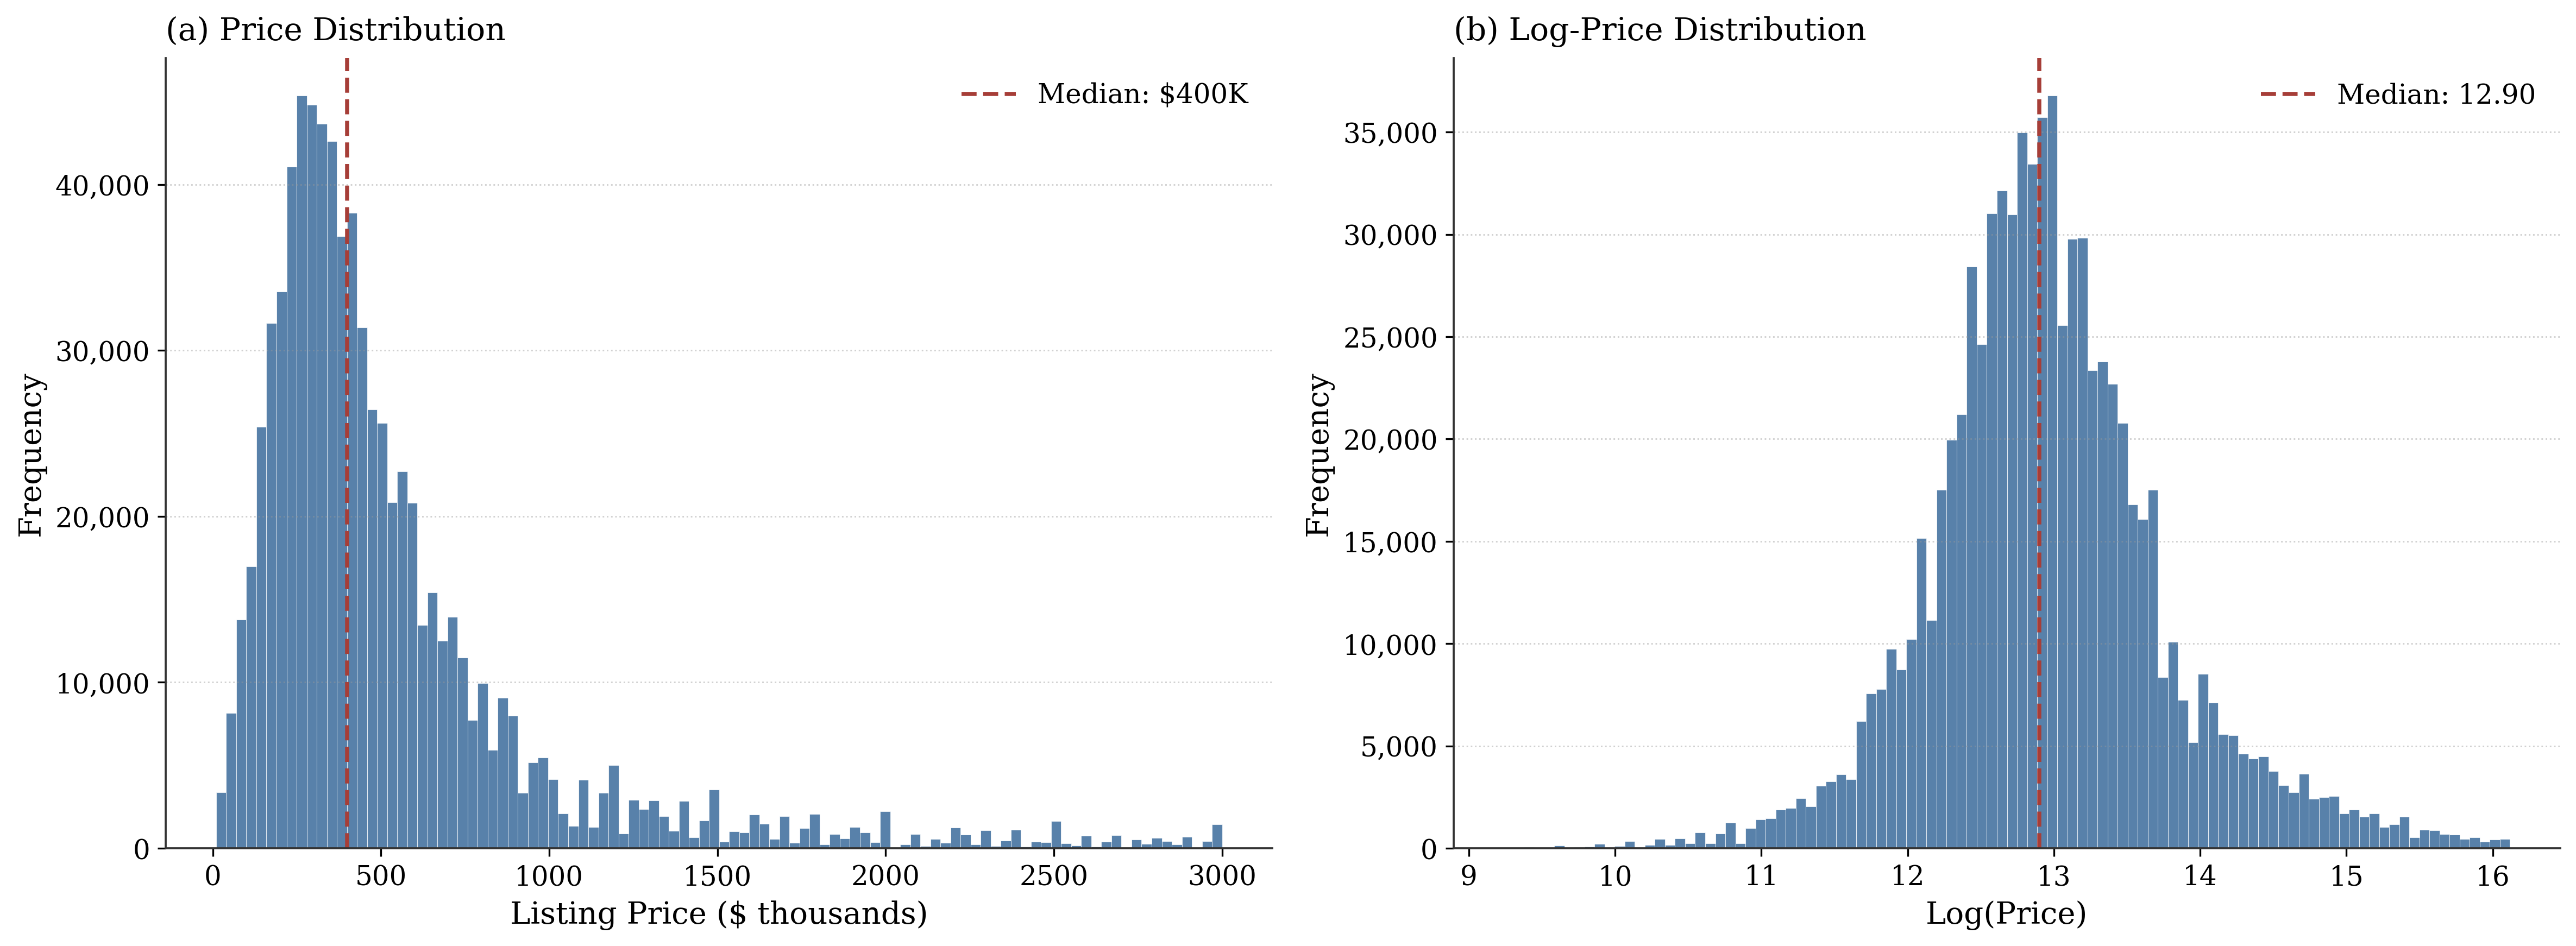
\includegraphics[width=\textwidth]{figures/fig1_price_distribution.png}
    \caption{Distribution of Listing Prices: (a) Levels; (b) Natural Logarithm. The log transformation reduces right skewness and approximates normality.}
    \label{fig:price_dist}
\end{figure}

% Author: Simon-Pierre Boucher — contact@spboucher.ai
%
% ═══════════════════════════════════════════════════════════════════════
% 4. METHODOLOGY
% ═══════════════════════════════════════════════════════════════════════
\section{Econometric and Machine Learning Methodology}
\label{sec:methodology}

\subsection{Identification, Prediction, and Interpretation}
\label{sec:identification}

Before presenting the estimation methods, we clarify the interpretive framework.

None of the models estimated in this paper identify causal willingness-to-pay parameters. OLS coefficients are conditional mean associations: they describe the average difference in log listing price between properties that differ by one unit in attribute $x_k$, holding other included attributes constant. Quantile regression coefficients are quantile-specific conditional associations. SHAP values are model-specific prediction decompositions. Table~\ref{tab:interpretation} summarizes these distinctions.

\begin{table}[H]
\centering
\caption{Interpretation of Estimates Across Modeling Frameworks}
\label{tab:interpretation}
\small
\begin{tabular}{lp{3.2cm}p{3.2cm}p{3.5cm}}
\toprule
& OLS Coefficient & Quantile Coefficient & SHAP Value \\
\midrule
Object & Cond.\ mean association & Cond.\ quantile association & Prediction contribution \\
Interpretation & Semi-elasticity (if unstandardized log-log) & Quantile-specific semi-elasticity & Model-specific contribution \\
Causal? & No, unless identified & No, unless identified & No \\
Structural WTP? & Only under strong assumptions & Only under strong assumptions & No \\
Primary use & Inference & Distributional heterogeneity & Prediction interpretation \\
\bottomrule
\end{tabular}
\end{table}

Cross-sectional data cannot separate preferences, supply constraints, and sorting. Regional and local omitted variables---including unobserved neighborhood quality, local supply conditions, and regulatory environment---remain major concerns. Throughout the paper, we interpret the estimates as \textbf{listing-price capitalization gradients} rather than structural demand parameters.

\subsection{Semi-Log Hedonic Specification (OLS)}

Our baseline model follows the semi-log specification:
\begin{equation}
    \ln(P_i) = \alpha + \sum_{k=1}^{K} \beta_k x_{ik} + \sum_{j=1}^{J} \gamma_j d_{ij} + \sum_{m=1}^{M} \delta_m (x_{im_1} \cdot x_{im_2}) + \varepsilon_i
    \label{eq:ols}
\end{equation}
where $P_i$ is the listing price, $x_{ik}$ are continuous and binary attributes, $d_{ij}$ are categorical dummies, and $x_{im_1} \cdot x_{im_2}$ are interaction terms.

\textbf{Coefficient interpretation under standardization.} All continuous regressors are standardized (zero mean, unit variance) prior to estimation. This facilitates coefficient magnitude comparison across variables with different scales but changes the interpretation: the coefficient on a standardized variable represents the association between a one-standard-deviation increase in the attribute and log-price, not a one-unit increase. In particular, the coefficient on standardized $\ln(\text{sqft})$ is \textit{not} a price-to-area elasticity---it is the effect of a one-standard-deviation increase in log living area. To recover economic magnitudes in natural units, we also report an unstandardized specification.

Binary (0/1) and dummy variables are not standardized. For these, the percentage listing-price effect is $(e^{\hat{\beta}_k} - 1) \times 100\%$.

Standard errors are computed using the HC3 estimator \citep{white1980heteroskedasticity, mackinnon1985some}.

\subsection{Quantile Regression}
\label{sec:qr_methodology}

Quantile regression \citep{koenker1978regression, koenker2001quantile} models the $\tau$-th conditional quantile:
\begin{equation}
    Q_{\tau}(\ln P_i | \mathbf{x}_i) = \mathbf{x}_i' \boldsymbol{\beta}(\tau), \quad \tau \in (0, 1)
\end{equation}
estimated by minimizing $\sum_{i} \rho_{\tau}(\ln P_i - \mathbf{x}_i' \boldsymbol{\beta})$, where $\rho_{\tau}(u) = u(\tau - \mathbb{1}(u < 0))$.

We estimate the model at $\tau \in \{0.10, 0.25, 0.50, 0.75, 0.90\}$. For computational tractability, estimation uses a random subsample of 150,000 observations. We verify stability by repeating estimation across ten random subsamples with different seeds, finding that most coefficients exhibit coefficient-of-variation below 8\% (Section~\ref{sec:qr_stability}).

\textbf{Inter-quantile Wald tests.} To formally test whether listing-price gradients differ between the lower and upper tails of the conditional distribution, we compute inter-quantile differences $\hat{\beta}_k(0.90) - \hat{\beta}_k(0.10)$ and test whether this difference is significantly different from zero using a $z$-test based on the covariance structure of the quantile regression estimates. Under the null hypothesis $H_0: \beta_k(0.90) = \beta_k(0.10)$, the test statistic is:
\begin{equation}
    z_k = \frac{\hat{\beta}_k(0.90) - \hat{\beta}_k(0.10)}{\sqrt{\text{Var}[\hat{\beta}_k(0.90)] + \text{Var}[\hat{\beta}_k(0.10)] - 2\,\text{Cov}[\hat{\beta}_k(0.90), \hat{\beta}_k(0.10)]}}
    \label{eq:iqr_test}
\end{equation}
Rejection indicates that the attribute's association with listing prices differs significantly between lower-priced and higher-priced properties (conditional on covariates).

\subsection{Gradient-Boosted Ensemble Models}

\subsubsection{XGBoost}

XGBoost \citep{chen2016xgboost} implements gradient boosting \citep{friedman2001greedy}, fitting an additive ensemble of regression trees by sequentially minimizing a regularized loss function:
\begin{equation}
    \mathcal{L}^{(t)} = \sum_{i=1}^{n} l(y_i, \hat{y}_i^{(t-1)} + f_t(\mathbf{x}_i)) + \Omega(f_t)
\end{equation}
where $\Omega(f_t) = \gamma T + \frac{1}{2}\lambda \|w\|^2 + \alpha \|w\|_1$ penalizes tree complexity. We use 1,000 trees, depth 8, learning rate 0.05, column and row subsampling ratios of 0.8, and early stopping after 50 rounds without improvement.

\subsubsection{LightGBM}

LightGBM \citep{ke2017lightgbm} uses Gradient-based One-Side Sampling (GOSS) and Exclusive Feature Bundling (EFB) for computational efficiency. We use matching hyperparameters for comparability.

\subsubsection{Additional Benchmarks}

We also report results for Ridge regression ($\alpha = 1$), Lasso ($\alpha = 0.001$), Elastic Net, Random Forest \citep[500 trees, depth 20;][]{breiman2001random}, and OLS with state fixed effects.

\textbf{Ablation design.} To understand which feature groups drive the ML predictive gain over OLS, we estimate XGBoost models using progressively richer feature sets: (i) structural attributes only (8 features); (ii) $+$ lot characteristics (9); (iii) $+$ amenity indicators (20); (iv) $+$ neighborhood variables (27); (v) $+$ market status (32); and (vi) the full model including interactions, categorical controls, and region dummies (62). At each stage, we evaluate both random and geographic holdout $R^2$ to identify which feature groups contribute to genuine predictive generalization versus spatial memorization.

\subsection{Validation Designs}
\label{sec:validation_designs}

Because housing prices are spatially dependent, the choice of validation protocol
is substantive rather than technical: random splits assess interpolation within
observed markets, while spatially blocked designs assess extrapolation to new
markets \citep{roberts2017cross, valavi2019blockcv, meyer2021predicting}. Blocked
validation is not universally preferable---for interpolation objectives it can be
pessimistically biased \citep{wadoux2021spatial}---so we report both protocols and
interpret each against its own deployment question. We employ three validation
strategies:

\begin{enumerate}[nosep]
    \item \textbf{Random 80/20 split} (seed = 42): 631,073 training, 157,769 test. This is the standard approach but permits spatial leakage---nearby properties from the same neighborhood can appear in both train and test sets.
    \item \textbf{Geographic holdout}: 10 states (CA, NY, TX, FL, OH, CO, NC, WA, IL, GA) are held out entirely; models are trained on the remaining 40 states + DC. This tests generalization to markets not seen during training. The held-out states represent the five largest (by sample size) plus five geographically diverse states, totaling 438,315 test observations.
    \item \textbf{Ablation cascade}: XGBoost models are estimated at six stages of feature inclusion under both random and geographic validation, isolating the marginal contribution of each feature group.
\end{enumerate}

The gap between random and geographic validation quantifies the extent to which models exploit local spatial structure rather than learning generalizable attribute-price relationships.

\subsection{SHAP-Based Model Interpretation and Cross-Model Stability}
\label{sec:shap_methodology}

SHAP values \citep{lundberg2017unified} decompose each prediction into additive feature contributions:
\begin{equation}
    f(\mathbf{x}) = E[f(\mathbf{X})] + \sum_{k=1}^{K} \phi_k(\mathbf{x})
\end{equation}
We compute TreeSHAP values on a random subsample of 10,000 test observations.

\textbf{Cross-model stability.} A common criticism of SHAP-based interpretation is that feature importance rankings may be model-specific. To assess this concern, we compute mean absolute SHAP values for three tree-based models (XGBoost, LightGBM, Random Forest) and report the Spearman rank correlation between each pair. High cross-model correlation would support the use of SHAP rankings as a description of the predictive structure of the data, not merely an artifact of a particular model.

\textbf{Interpretive caution.} SHAP values are prediction-level contributions, not structural implicit prices. They are:
\begin{itemize}[nosep]
    \item model-dependent (XGBoost SHAP values differ from LightGBM SHAP values);
    \item affected by feature correlation (correlated features may share SHAP contributions);
    \item not causal---they decompose predictions, not data-generating processes;
    \item not equivalent to Rosen's hedonic price gradient $\partial P / \partial z_k$.
\end{itemize}
We use SHAP to describe which features contribute most to predictions, not to estimate marginal willingness to pay.

\subsection{Spatial Autocorrelation Diagnostics}
\label{sec:moran_method}

We compute Moran's $I$ \citep{moran1950notes} on OLS residuals using a row-standardized KNN spatial weight matrix ($k = 8$) on random subsamples of 5,000 observations. To assess the stability of this diagnostic, we repeat the computation across three independent subsamples and report the mean, standard deviation, and significance of the resulting $I$ statistics. Moran's $I$ is defined as:
\begin{equation}
    I = \frac{N}{\sum_{i}\sum_{j} w_{ij}} \cdot \frac{\sum_{i}\sum_{j} w_{ij}(e_i - \bar{e})(e_j - \bar{e})}{\sum_{i}(e_i - \bar{e})^2}
    \label{eq:moran}
\end{equation}
where $e_i$ are the OLS residuals, $w_{ij}$ are the spatial weights, and $N$ is the subsample size. Under the null of no spatial autocorrelation, $I$ has expected value $-1/(N-1) \approx 0$ and an asymptotically normal distribution. Values significantly above zero indicate positive spatial autocorrelation (nearby residuals are similar), implying that the OLS specification fails to capture local price variation.

% Author: Simon-Pierre Boucher — contact@spboucher.ai
%
% ═══════════════════════════════════════════════════════════════════════
% 5. RESULTS
% ═══════════════════════════════════════════════════════════════════════
\section{Estimation Results}
\label{sec:results}

\subsection{OLS Baseline, State Fixed Effects, and ZIP3 Fixed Effects}
\label{sec:ols_fe}

\subsubsection{Standardized Baseline Specification}

Table~\ref{tab:ols_results} presents the OLS results with standardized continuous regressors. The model achieves $R^2 = 0.634$ with RMSE $= 0.489$ in log-price units. The $F$-statistic of 18,712.5 strongly rejects the null of jointly zero slope coefficients.

\begin{table}[H]
\centering
\caption{OLS Hedonic Regression Results (Dep.\ Var.: $\ln(\text{Listing Price})$)}
\label{tab:ols_results}
\begin{threeparttable}
\small
\begin{tabular}{lrrl}
\toprule
Variable & Coefficient & Std.\ Error & \\
\midrule
\multicolumn{4}{l}{\textit{Panel A: Structural Attributes (standardized)}} \\
$\ln$(Living Area)$^\dagger$ & 0.3119 & 0.0035 & *** \\
Bedrooms$^\dagger$ & $-$0.0675 & 0.0023 & *** \\
Bathrooms$^\dagger$ & 0.2359 & 0.0026 & *** \\
Age$^\dagger$ & $-$0.0418 & 0.0139 & ** \\
Age$^{2\dagger}$ & 0.0507 & 0.0019 & *** \\
Stories$^\dagger$ & 0.0004 & 0.0003 & \\
Bath/Bed Ratio$^\dagger$ & $-$0.0208 & 0.0021 & *** \\
\midrule
\multicolumn{4}{l}{\textit{Panel B: Lot and Amenities}} \\
$\ln$(Lot Size)$^\dagger$ & 0.0697 & 0.0010 & *** \\
Pool & 0.0286 & 0.0026 & *** \\
Spa & 0.0327 & 0.0027 & *** \\
Basement & $-$0.0424 & 0.0023 & *** \\
Garage & 0.1094 & 0.0015 & *** \\
Waterfront & $-$0.1349 & 0.0325 & *** \\
Central Air & 0.0693 & 0.0014 & *** \\
Hardwood Floors & 0.1246 & 0.0014 & *** \\
Luxury Score$^\dagger$ & 0.0443 & 0.0018 & *** \\
\midrule
\multicolumn{4}{l}{\textit{Panel C: Neighborhood (standardized)}} \\
Walk Score$^\dagger$ & $-$0.0109 & 0.0012 & *** \\
Bike Score$^\dagger$ & 0.0717 & 0.0010 & *** \\
Transit Score$^\dagger$ & 0.0524 & 0.0008 & *** \\
Avg.\ School Rating$^\dagger$ & $-$0.0491 & 0.0007 & *** \\
Property Tax Rate$^\dagger$ & $-$0.0292 & 0.0008 & *** \\
\midrule
\multicolumn{4}{l}{\textit{Panel D: Market Status}} \\
Condominium & $-$0.0370 & 0.0037 & *** \\
HOA Member & $-$0.1077 & 0.0024 & *** \\
$\ln$(HOA Fees + 1)$^\dagger$ & 0.0439 & 0.0014 & *** \\
New Construction & 0.1035 & 0.0029 & *** \\
Foreclosure & $-$0.4064 & 0.0098 & *** \\
\midrule
\multicolumn{4}{l}{\textit{Panel E: Interactions (standardized)}} \\
$\ln$(sqft) $\times$ Age$^\dagger$ & $-$0.1100 & 0.0140 & *** \\
Pool $\times$ South & 0.0081 & 0.0012 & *** \\
Waterfront $\times$ $\ln$(sqft)$^\dagger$ & 0.1371 & 0.0092 & *** \\
Basement $\times$ North & $-$0.0255 & 0.0012 & *** \\
Condo $\times$ Walk Score$^\dagger$ & 0.0816 & 0.0013 & *** \\
Age $\times$ Luxury$^\dagger$ & 0.0440 & 0.0015 & *** \\
\midrule
\multicolumn{4}{l}{\textit{Panel F: Regional Dummies (ref: Midwest)}} \\
Northeast & 0.4869 & 0.0030 & *** \\
South & 0.0220 & 0.0028 & *** \\
West & 0.4008 & 0.0031 & *** \\
\midrule
$R^2$ & 0.6343 & & \\
Adj.\ $R^2$ & 0.6342 & & \\
RMSE & 0.4887 & & \\
$F$-statistic & 18,712.5 & & \\
$N$ & 788,842 & & \\
\bottomrule
\end{tabular}
\begin{tablenotes}
\small
\item \textit{Notes:} HC3 heteroskedasticity-robust standard errors. $^\dagger$Variables standardized (zero mean, unit variance) before estimation; coefficients represent effects of a one-standard-deviation increase. Binary variables not standardized; percentage effects computed as $100 \times (e^\beta - 1)$. Categorical controls (roof: 6, construction: 8, foundation: 7 dummies) included but not shown. Significance: *** $p<0.001$, ** $p<0.01$, * $p<0.05$.
\end{tablenotes}
\end{threeparttable}
\end{table}

\subsubsection{Unstandardized Specification for Economic Interpretation}

Table~\ref{tab:ols_unstd} reports key coefficients from the unstandardized specification, which permits direct economic interpretation. The $R^2$ is identical (0.634); only the coefficient magnitudes and interpretations differ.

\begin{table}[H]
\centering
\caption{Unstandardized OLS: Key Coefficients in Natural Units}
\label{tab:ols_unstd}
\begin{threeparttable}
\small
\begin{tabular}{lrrrl}
\toprule
Variable & Coefficient & Std.\ Error & Interpretation & \\
\midrule
Constant & 7.7316 & 0.0495 & & *** \\
$\ln$(Living Area) & 0.6281 & 0.0070 & Elasticity: 0.63 & *** \\
Bedrooms & $-$0.0620 & 0.0022 & $-$6.0\% per additional bedroom & *** \\
Bathrooms & 0.2035 & 0.0023 & +22.6\% per additional bathroom & *** \\
Age (years) & $-$0.0013 & 0.0004 & $-$0.13\% per year & ** \\
Age$^2$ ($\times 10^{-5}$) & 1.2 & 0.05 & Positive quadratic (vintage) & *** \\
$\ln$(Lot Size) & 0.0182 & 0.0003 & Elasticity: 0.02 & *** \\
Walk Score (per point) & $-$0.0004 & 0.0000 & $-$0.04\% per point & *** \\
Bike Score (per point) & 0.0040 & 0.0001 & +0.40\% per point & *** \\
Transit Score (per point) & 0.0029 & 0.0000 & +0.29\% per point & *** \\
Avg.\ School Rating (per point) & $-$0.0544 & 0.0008 & $-$5.3\% per rating point & *** \\
Property Tax Rate (per ppt) & $-$0.0553 & 0.0015 & $-$5.4\% per ppt & *** \\
Luxury Score (per unit) & 0.0344 & 0.0014 & +3.5\% per unit & *** \\
\bottomrule
\end{tabular}
\begin{tablenotes}
\small
\item \textit{Notes:} Same sample and specification as Table~\ref{tab:ols_results}, but continuous variables enter in natural units. $N = 788{,}842$. HC3 standard errors.
\end{tablenotes}
\end{threeparttable}
\end{table}

The elasticity of listing price with respect to living area is 0.63: a 10\% increase in square footage is associated with a 6.3\% higher listing price. This is below unity, consistent with diminishing marginal returns to space. Each additional bathroom is associated with a 22.6\% higher listing price, while each additional bedroom---conditional on total area---is associated with a 6.0\% \textit{lower} price, reflecting the well-documented tradeoff between room count and room size \citep{sirmans2005composition}.

\subsubsection{Counterintuitive Coefficient Signs}

Several coefficients warrant discussion.

\textbf{Negative waterfront coefficient ($-0.135$, standardized).} The standalone waterfront effect is evaluated at the mean of the standardized interaction term $\text{waterfront} \times \ln(\text{sqft})$. Because the interaction is strongly positive ($+0.137$), the net waterfront effect becomes positive for larger properties. This artifact of the interacted specification does not imply that waterfront reduces price on average.

\textbf{Negative school rating ($-0.054$ per rating point, unstandardized).} This likely reflects confounding with property tax rates and regional effects. In higher-tax jurisdictions, school quality is partially capitalized through the tax rate, which enters separately. Conditional on tax rate, region, and other controls, the residual school rating variation may capture unobserved factors that correlate negatively with prices. The boundary-discontinuity literature, which isolates school quality from neighborhood composition, consistently finds positive valuations \citep{black1999better, bayer2007unified}; the divergence illustrates why cross-sectional partial coefficients on school quality should not be interpreted structurally.

\textbf{Negative Walk Score ($-0.0004$ per point, unstandardized).} Walk Score is highly correlated with Bike Score ($r \approx 0.56$) and Transit Score ($r \approx 0.62$). In the presence of all three accessibility measures, the Walk Score coefficient may reflect residual urban density effects---after controlling for biking and transit access, the remaining variation in walkability may capture denser, smaller-lot neighborhoods. A walkability premium is well documented when accessibility enters alone \citep{pivo2011walkability}; with three collinear accessibility scores, the premium is split across coefficients and cannot be attributed variable-by-variable.

\textbf{Negative basement ($-0.042$).} Basements are predominantly found in older properties in colder regions. Conditional on age, region, and size, the basement indicator may proxy for older construction quality or layout features valued less in modern markets.

\textbf{Negative HOA membership ($-0.108$).} HOA properties include condominiums and planned communities that may have lower lot sizes and more restrictions. The negative sign is conditional on the separate log HOA fee variable ($+0.044$), suggesting that the HOA membership dummy captures the property-type effect while fees capture the service-quality gradient.

These counterintuitive signs are common in hedonic regressions with many correlated controls and do not necessarily indicate misspecification, though they do limit the attributable economic interpretation of individual coefficients.

\subsubsection{Progressive Geographic Fixed Effects}
\label{sec:progressive_fe}

Table~\ref{tab:fe_comparison} documents how explanatory power increases with geographic granularity. Adding 50 state fixed effects increases the in-sample $R^2$ from 0.634 to 0.681. Replacing state dummies with 886 ZIP3 fixed effects further increases $R^2$ to 0.729 (in-sample) and out-of-sample $R^2$ to 0.725.

\begin{table}[H]
\centering
\caption{OLS $R^2$ Under Progressively Finer Geographic Controls}
\label{tab:fe_comparison}
\begin{threeparttable}
\begin{tabular}{lrrrr}
\toprule
Specification & Geographic FE & $N_{\text{FE}}$ & In-sample $R^2$ & Out-of-sample $R^2$ \\
\midrule
Baseline (4 regions) & Census Region & 3 & 0.634 & 0.630 \\
State FE & State & 50 & 0.681 & 0.678 \\
ZIP3 FE & 3-digit ZIP & 886 & 0.729 & 0.725 \\
\bottomrule
\end{tabular}
\begin{tablenotes}
\small
\item \textit{Notes:} Same 62 non-geographic regressors across all specifications; geographic FE replace the 3 regional dummies. Out-of-sample $R^2$ computed on a random 20\% holdout. ZIP3 codes cover 886 unique prefixes in the sample.
\end{tablenotes}
\end{threeparttable}
\end{table}

The progression from region to state to ZIP3 fixed effects yields $R^2$ gains of $+4.7$ pp and $+4.7$ pp, respectively. This 9.5 pp total gain from geographic granularity alone---achieved without any additional property-level information---underscores the importance of unobserved local factors in hedonic pricing. Notably, even ZIP3 fixed effects leave substantial residual variation unexplained: the gap between ZIP3 OLS ($R^2 = 0.725$) and XGBoost under random validation ($R^2 = 0.833$) suggests that non-linear attribute effects contribute an additional 10.8 pp of explained variation.

\subsubsection{OLS Diagnostics}

Figure~\ref{fig:diagnostics} presents diagnostic plots. The residual distribution exhibits excess kurtosis (5.55 vs.\ 3.0 for normality) and mild positive skewness (0.18), as confirmed by the Jarque-Bera test ($JB = 217{,}078$, $p < 0.001$). The heteroskedastic pattern visible in the residuals-versus-fitted plot motivates our use of HC3 standard errors.

\begin{figure}[H]
    \centering
    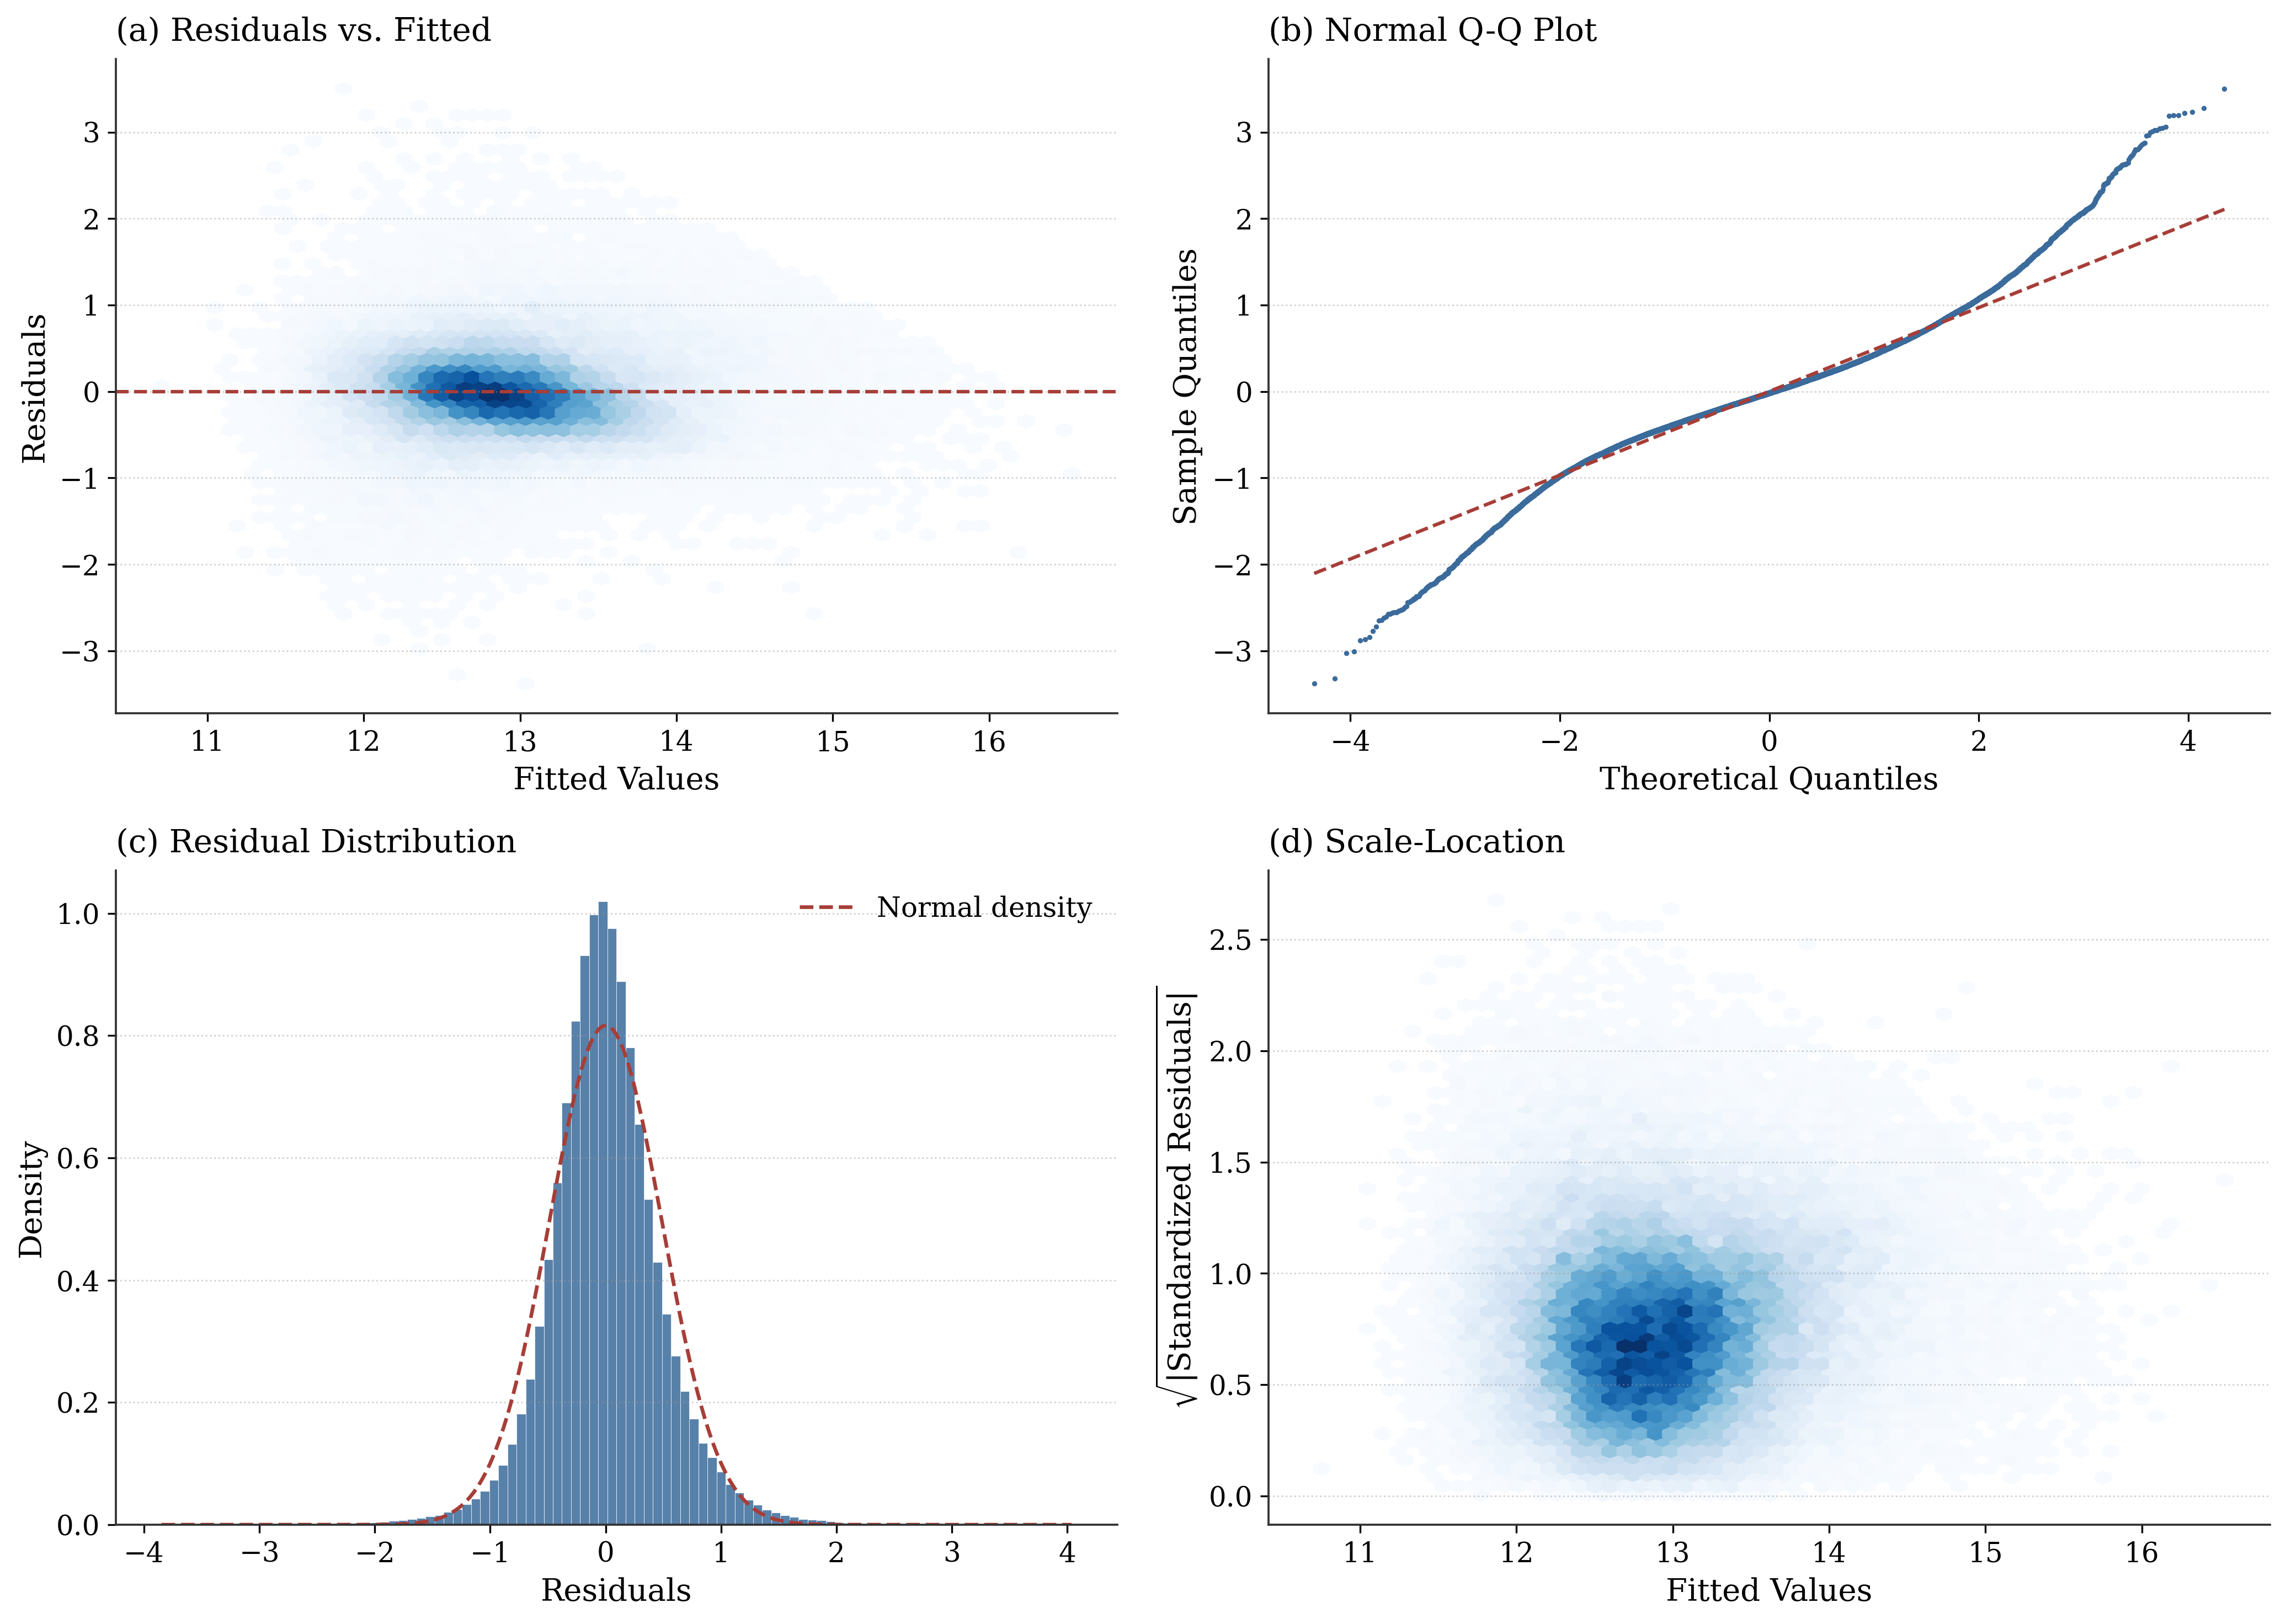
\includegraphics[width=\textwidth]{figures/fig2_ols_diagnostics.png}
    \caption{OLS Diagnostic Plots: (a) Residuals vs.\ Fitted; (b) Normal Q-Q Plot; (c) Residual Distribution; (d) Scale-Location}
    \label{fig:diagnostics}
\end{figure}


\subsection{Spatial Autocorrelation}
\label{sec:spatial_autocorrelation}

We compute Moran's $I$ on OLS residuals using a KNN spatial weight matrix ($k = 8$) on three independent random subsamples of 5,000 observations each. Table~\ref{tab:moran} reports the results.

\begin{table}[H]
\centering
\caption{Moran's $I$ on OLS Residuals: Subsample Stability}
\label{tab:moran}
\begin{threeparttable}
\begin{tabular}{lrrrl}
\toprule
Subsample & $I$ & $z$-statistic & $p$-value & \\
\midrule
Subsample 1 & 0.2742 & 41.8 & $<0.001$ & *** \\
Subsample 2 & 0.2839 & 43.5 & $<0.001$ & *** \\
Subsample 3 & 0.2652 & 40.5 & $<0.001$ & *** \\
\midrule
Mean & 0.2745 & & & \\
Std.\ Dev. & 0.0076 & & & \\
\bottomrule
\end{tabular}
\begin{tablenotes}
\small
\item \textit{Notes:} Row-standardized KNN weight matrix with $k = 8$. Each subsample draws 5,000 observations at random. All $z$-statistics strongly reject the null of no spatial autocorrelation. The low standard deviation (0.008) across subsamples indicates that the diagnostic is highly stable.
\end{tablenotes}
\end{threeparttable}
\end{table}

The mean Moran's $I = 0.2745$ (std $= 0.0076$) across three subsamples confirms \textbf{strong, stable positive spatial autocorrelation} in the OLS residuals. This implies that our regional controls (four Census regions) are insufficient to absorb local price variation. OLS standard errors may understate true uncertainty, and coefficient estimates may be biased if the spatial structure correlates with included regressors. The stability across subsamples (CV $= 2.8\%$) indicates that this is not a sampling artifact but a structural feature of the data. Addressing spatial dependence through spatial econometric models is an important direction for future work; our OLS and quantile regression results should be interpreted with this caveat.


\subsection{Quantile Regression and Inter-Quantile Tests}
\label{sec:qr_results}

\subsubsection{Coefficient Estimates Across Quantiles}

Table~\ref{tab:qr_results} presents quantile regression coefficients at the five estimated quantiles.

\begin{table}[H]
\centering
\caption{Quantile Regression Coefficients at Selected Quantiles}
\label{tab:qr_results}
\begin{threeparttable}
\small
\begin{tabular}{lrrrrrr}
\toprule
Variable & $\tau=0.10$ & $\tau=0.25$ & $\tau=0.50$ & $\tau=0.75$ & $\tau=0.90$ & OLS \\
\midrule
$\ln$(Living Area) & 0.358*** & 0.313*** & 0.275*** & 0.237*** & 0.251*** & 0.312*** \\
Bedrooms & $-$0.085*** & $-$0.076*** & $-$0.064*** & $-$0.037*** & $-$0.034*** & $-$0.068*** \\
Bathrooms & 0.157*** & 0.195*** & 0.234*** & 0.259*** & 0.259*** & 0.236*** \\
Age & $-$0.430*** & $-$0.201*** & $-$0.066** & $-$0.007 & $-$0.026 & $-$0.042** \\
$\ln$(Lot Size) & 0.045*** & 0.051*** & 0.061*** & 0.070*** & 0.086*** & 0.070*** \\
Pool & 0.008 & 0.008 & 0.019*** & 0.061*** & 0.094*** & 0.029*** \\
Garage & 0.205*** & 0.146*** & 0.102*** & 0.061*** & 0.020*** & 0.109*** \\
Luxury Score & 0.018*** & 0.038*** & 0.054*** & 0.068*** & 0.072*** & 0.044*** \\
Foreclosure & $-$0.494*** & $-$0.473*** & $-$0.379*** & $-$0.327*** & $-$0.338*** & $-$0.406*** \\
Northeast & 0.339*** & 0.395*** & 0.471*** & 0.553*** & 0.603*** & 0.487*** \\
West & 0.365*** & 0.372*** & 0.376*** & 0.399*** & 0.450*** & 0.401*** \\
\bottomrule
\end{tabular}
\begin{tablenotes}
\small
\item \textit{Notes:} Estimated on a random subsample of 150,000 observations. Continuous variables standardized. Full set of 62 regressors included; selected coefficients shown. Significance: *** $p<0.001$, ** $p<0.01$, * $p<0.05$. Coefficients reflect one-standard-deviation effects for continuous variables.
\end{tablenotes}
\end{threeparttable}
\end{table}

\begin{figure}[H]
    \centering
    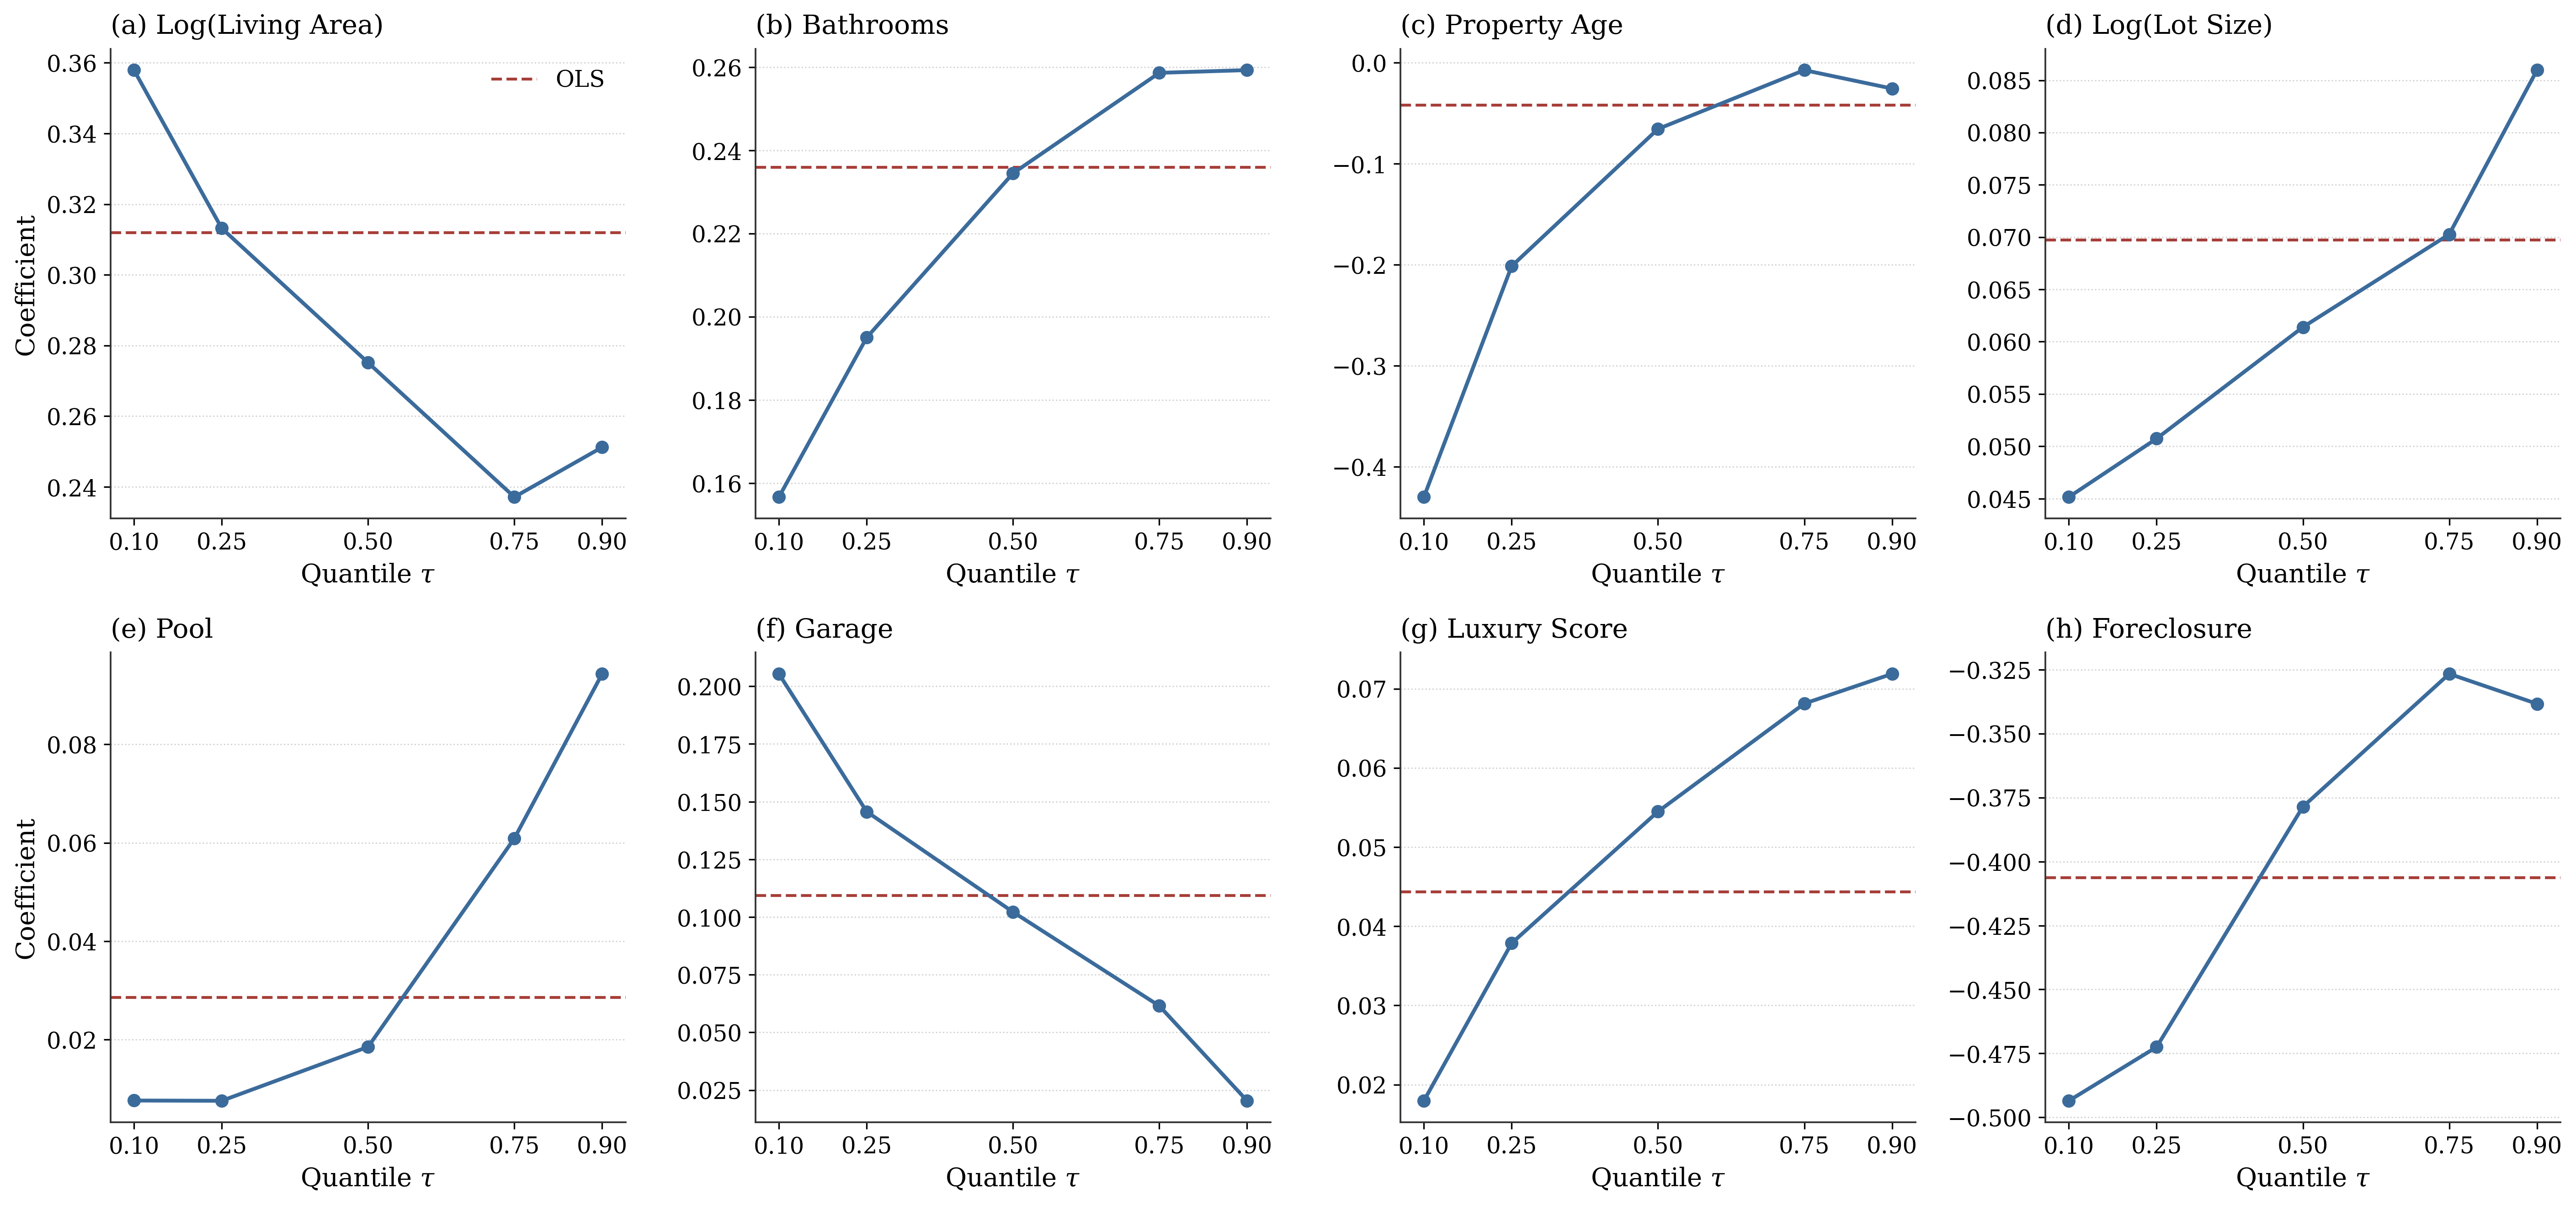
\includegraphics[width=\textwidth]{figures/fig3_quantile_coefficients.png}
    \caption{Quantile Regression Coefficients Across the Conditional Price Distribution. Red dashed lines indicate OLS estimates. Coefficients are on standardized variables.}
    \label{fig:qr_coefficients}
\end{figure}

Several economically interesting patterns emerge.

\textbf{Living area gradient declines at upper quantiles.} The standardized $\ln(\text{sqft})$ coefficient declines from 0.358 ($\tau = 0.10$) to 0.237 ($\tau = 0.75$), indicating that additional space is associated with proportionally larger listing-price differences at the lower end of the conditional distribution. At higher quantiles, other factors (luxury features, location) may dominate size.

\textbf{Bathroom gradient increases at upper quantiles.} In contrast, the bathroom gradient rises monotonically from 0.157 ($\tau = 0.10$) to 0.259 ($\tau = 0.90$), suggesting that bathroom count differentiates properties more strongly in the upper market.

\textbf{Age penalty concentrated at lower quantiles.} The age gradient is $-0.430$ at $\tau = 0.10$ but statistically insignificant at $\tau = 0.75$ and $\tau = 0.90$. Age-related depreciation appears to be primarily a phenomenon of lower-priced properties, possibly because higher-priced properties are better maintained or benefit from vintage appeal.

\textbf{Pool gradient emerges only above the median.} The pool coefficient is insignificant at $\tau = 0.10$ and $\tau = 0.25$ but rises to 0.094 at $\tau = 0.90$ ($\approx 9.9\%$ listing-price difference), consistent with pools being a luxury amenity.

\textbf{Garage gradient declines monotonically.} The garage coefficient drops from 0.205 ($\tau = 0.10$) to 0.020 ($\tau = 0.90$), reflecting that garage availability differentiates lower-priced properties much more than upper-priced ones where garages are nearly universal.

OLS averages across these heterogeneous gradients and can therefore misrepresent both the lower and upper segments of the market.

\subsubsection{Inter-Quantile Wald Tests ($\tau = 0.10$ vs.\ $\tau = 0.90$)}

Table~\ref{tab:iqr_tests} reports the inter-quantile Wald tests for equality of coefficients between the 10th and 90th percentiles.

\begin{table}[H]
\centering
\caption{Inter-Quantile Wald Tests: $\hat{\beta}(0.10) - \hat{\beta}(0.90)$}
\label{tab:iqr_tests}
\begin{threeparttable}
\small
\begin{tabular}{lrrrl}
\toprule
Variable & $\hat{\beta}(0.10) - \hat{\beta}(0.90)$ & $z$-statistic & $p$-value & \\
\midrule
Garage & $+$0.185 & 28.92 & $<0.001$ & *** \\
Northeast & $-$0.264 & $-$21.43 & $<0.001$ & *** \\
Bathrooms & $-$0.103 & $-$10.48 & $<0.001$ & *** \\
$\ln$(Living Area) & $+$0.107 & 9.52 & $<0.001$ & *** \\
$\ln$(Lot Size) & $-$0.041 & $-$9.49 & $<0.001$ & *** \\
Age & $-$0.405 & $-$7.89 & $<0.001$ & *** \\
Pool & $-$0.087 & $-$7.80 & $<0.001$ & *** \\
Luxury Score & $-$0.054 & $-$6.82 & $<0.001$ & *** \\
West & $-$0.086 & $-$6.26 & $<0.001$ & *** \\
Bedrooms & $-$0.051 & $-$5.95 & $<0.001$ & *** \\
Foreclosure & $-$0.155 & $-$4.18 & $<0.001$ & *** \\
\midrule
\multicolumn{5}{l}{\textit{Not significant ($p > 0.05$)}} \\
Waterfront & $+$0.222 & 1.86 & 0.063 & \\
Age$^2$ & $+$0.010 & 1.40 & 0.162 & \\
\bottomrule
\end{tabular}
\begin{tablenotes}
\small
\item \textit{Notes:} $z$-statistics computed from the joint covariance matrix of the $\tau = 0.10$ and $\tau = 0.90$ quantile regression estimates; both quantiles estimated on the same 150,000-observation subsample. Variables sorted by $|z|$. 11 of 13 tested variables show statistically significant differences at the 5\% level. *** $p<0.001$, ** $p<0.01$, * $p<0.05$.
\end{tablenotes}
\end{threeparttable}
\end{table}

The inter-quantile tests reject coefficient equality for 11 of 13 tested variables at the 5\% level. The largest inter-quantile difference is for garage ($+0.185$, $z = 28.92$), confirming that the garage listing-price gradient is dramatically larger for lower-priced properties. Bathrooms ($-0.103$, $z = -10.48$) and living area ($+0.107$, $z = 9.52$) also exhibit large, highly significant inter-quantile differences. The only two variables for which the null of equal coefficients cannot be rejected are age-squared ($z = 1.40$) and waterfront ($z = 1.86$, $p = 0.063$).

These formal tests confirm the visual patterns in Figure~\ref{fig:qr_coefficients}: the conditional distribution of listing prices is not merely shifted by housing attributes but is differentially stretched and compressed, with different attributes mattering more at different points in the distribution.


\subsection{Machine Learning Under Random Validation}
\label{sec:ml_random}

Table~\ref{tab:ml_comparison} summarizes out-of-sample performance under the random 80/20 split.

\begin{table}[H]
\centering
\caption{Out-of-Sample Predictive Performance: Random Validation}
\label{tab:ml_comparison}
\begin{threeparttable}
\small
\begin{tabular}{lrrrrrr}
\toprule
 & \multicolumn{3}{c}{Log-Price Scale} & \multicolumn{3}{c}{Dollar Scale} \\
\cmidrule(lr){2-4} \cmidrule(lr){5-7}
Model & $R^2$ & RMSE & MAE & MAPE (\%) & MdAPE (\%) & MAE (\$) \\
\midrule
OLS & 0.6301 & 0.4911 & 0.3619 & 39.8 & 27.2 & 240,941 \\
Ridge ($\alpha=1$) & 0.6301 & 0.4911 & 0.3619 & --- & --- & --- \\
Lasso ($\alpha=0.001$) & 0.6280 & 0.4925 & 0.3627 & --- & --- & --- \\
Elastic Net & 0.6145 & 0.5014 & 0.3681 & --- & --- & --- \\
OLS + State FE & 0.6775 & 0.4586 & --- & --- & --- & --- \\
OLS + ZIP3 FE & 0.7253 & --- & --- & --- & --- & --- \\
Random Forest & 0.7842 & 0.3751 & 0.2636 & 28.4 & 18.5 & 180,116 \\
LightGBM & 0.8088 & 0.3531 & 0.2519 & 26.9 & 18.2 & 169,495 \\
\textbf{XGBoost} & \textbf{0.8330} & \textbf{0.3300} & \textbf{0.2327} & \textbf{24.7} & \textbf{16.5} & \textbf{157,822} \\
\bottomrule
\end{tabular}
\begin{tablenotes}
\small
\item \textit{Notes:} Training: 631,073 (80\%). Test: 157,769 (20\%). Random split, seed 42. MAPE = mean absolute percentage error; MdAPE = median APE. Dollar metrics computed by exponentiating predicted log-prices. Ridge, Lasso, Elastic Net dollar metrics suppressed for brevity (similar to OLS). ZIP3 FE RMSE and dollar-scale metrics not computed for this specification.
\end{tablenotes}
\end{threeparttable}
\end{table}

XGBoost achieves the highest $R^2$ of 0.833 under random validation, representing a 20-percentage-point improvement over OLS. Regularized linear models (Ridge, Lasso, Elastic Net) offer no improvement over OLS, confirming that the parametric specification is not overfit---the predictive gap is driven by non-linearity and interaction effects, not overfitting. The ZIP3 FE model ($R^2 = 0.725$) closes roughly half the OLS-to-XGBoost gap, indicating that fine-grained geographic controls capture a substantial portion of the non-linearity that tree models exploit.

\begin{figure}[H]
    \centering
    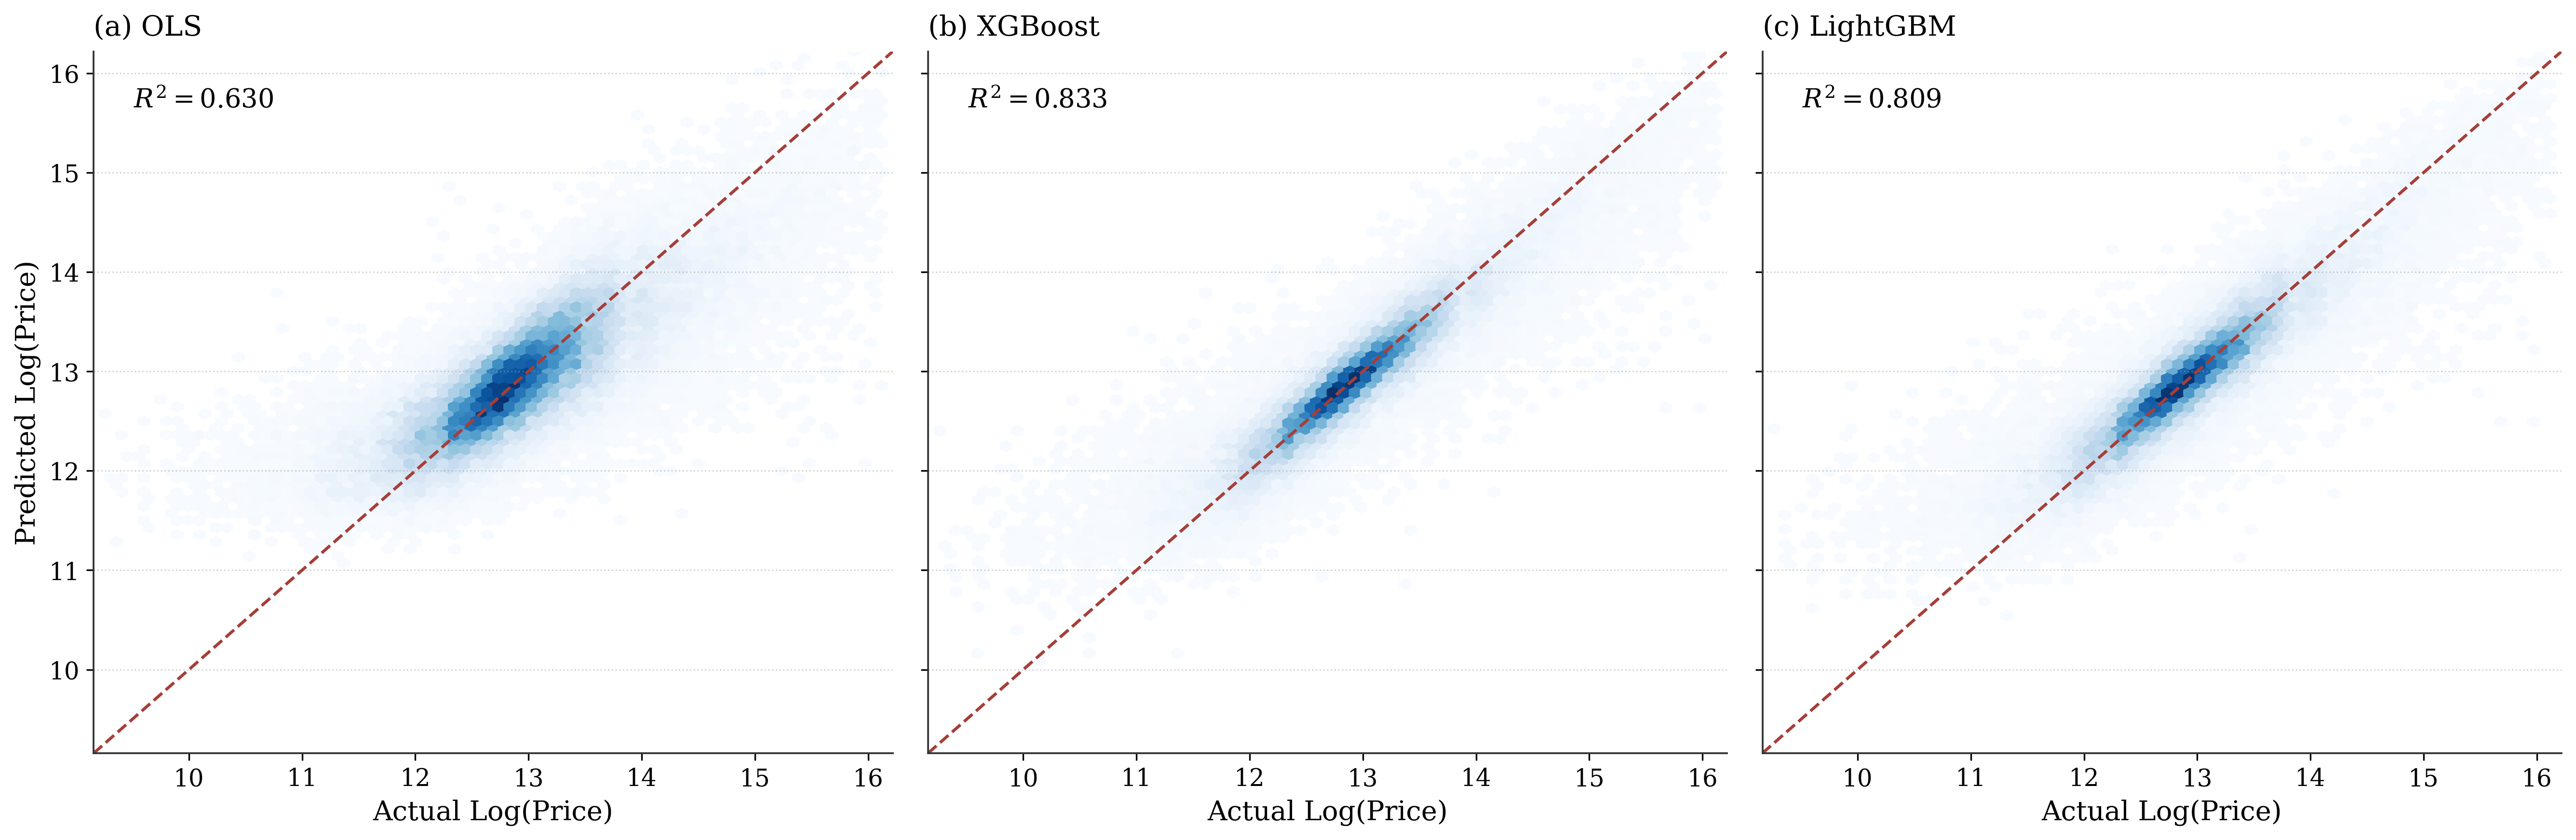
\includegraphics[width=\textwidth]{figures/fig4_model_comparison.png}
    \caption{Predicted vs.\ Actual Log-Prices Under Random Validation: (a) OLS; (b) XGBoost; (c) LightGBM}
    \label{fig:model_comparison}
\end{figure}


\subsection{Machine Learning Under Geographic Validation}
\label{sec:ml_geo}

Table~\ref{tab:geo_holdout} reports performance when 10 states are held out entirely.

\begin{table}[H]
\centering
\caption{Geographic Holdout Validation (10 States Held Out)}
\label{tab:geo_holdout}
\begin{threeparttable}
\begin{tabular}{lrrr}
\toprule
Model & $R^2$ (random) & $R^2$ (geo holdout) & $\Delta R^2$ \\
\midrule
OLS & 0.630 & $<0$ & $>-0.63$ \\
Random Forest & 0.784 & 0.542 & $-0.242$ \\
XGBoost & 0.833 & 0.547 & $-0.286$ \\
XGBoost (no geo features) & 0.830 & 0.519 & $-0.311$ \\
XGBoost (+ lat/lon) & 0.870 & 0.464 & $-0.406$ \\
\bottomrule
\end{tabular}
\begin{tablenotes}
\small
\item \textit{Notes:} Geographic holdout: CA, NY, TX, FL, OH, CO, NC, WA, IL, GA held out (438,315 observations). Training on remaining 350,527 observations. OLS with regional dummies fails catastrophically because the held-out states span all four Census regions and include the largest markets. ``No geo features'' removes region dummies from the full model. ``+ lat/lon'' adds raw latitude and longitude as continuous features.
\end{tablenotes}
\end{threeparttable}
\end{table}

\textbf{Key finding.} The XGBoost $R^2$ drops from 0.833 (random) to 0.547 (geographic holdout)---a \textbf{28.6-percentage-point decline}. This demonstrates that a substantial portion of the random-validation $R^2$ reflects the model's ability to exploit local spatial structure rather than learning generalizable attribute-price relationships.

Two additional experiments sharpen this conclusion:
\begin{itemize}[nosep]
    \item \textbf{Adding latitude and longitude} boosts random $R^2$ from 0.833 to 0.870 ($+3.7$ pp) but \emph{reduces} geographic holdout $R^2$ to 0.464 ($-8.3$ pp relative to the baseline XGBoost). Coordinates allow the model to memorize location-specific price levels, which is useful when nearby properties appear in the test set but harmful when entire states are withheld.
    \item \textbf{Removing all geographic features} (no region dummies) yields random $R^2 = 0.830$ (essentially unchanged) but geographic holdout $R^2 = 0.519$. Compared to the ablation-design variant of the full model (Geo $R^2 = 0.425$; see Section~\ref{sec:ablation}), dropping geography \emph{improves} geographic holdout by $+9.4$ pp. Region dummies can \emph{harm} geographic generalization because they encode training-set-specific geographic price levels.
\end{itemize}

This finding is methodologically important: \textbf{random train-test splits can substantially overstate the predictive performance of hedonic models} when applied to geographically diverse national samples. Geographic holdout validation provides a more conservative---and arguably more relevant---assessment of model generalizability.


\subsection{Ablation: What Drives the ML Gain?}
\label{sec:ablation}

Table~\ref{tab:ablation} presents the results of the feature ablation analysis for XGBoost.

\begin{table}[H]
\centering
\caption{XGBoost Ablation Analysis: Marginal Contribution of Feature Groups}
\label{tab:ablation}
\begin{threeparttable}
\small
\begin{tabular}{llrrrr}
\toprule
Stage & Feature Set & $N_{\text{features}}$ & Random $R^2$ & Geo $R^2$ & $\Delta$ Geo $R^2$ \\
\midrule
1 & Structural only & 8 & 0.4976 & 0.3481 & --- \\
2 & + Lot & 9 & 0.5464 & 0.3765 & $+$0.028 \\
3 & + Amenities & 20 & 0.6378 & 0.4485 & $+$0.072 \\
4 & + Neighborhood & 27 & 0.8136 & 0.4833 & $+$0.035 \\
5 & + Market status & 32 & 0.8235 & 0.5014 & $+$0.018 \\
6 & Full model (+ interactions/cats/region) & 62 & 0.8327 & 0.4250 & $-$0.076 \\
\bottomrule
\end{tabular}
\begin{tablenotes}
\small
\item \textit{Notes:} Each row adds a feature group to the previous stage. Random $R^2$ is computed on the standard 20\% random holdout. Geo $R^2$ is computed on the 10-state geographic holdout. $\Delta$ Geo $R^2$ is the change from the previous stage.
\end{tablenotes}
\end{threeparttable}
\end{table}

Three findings emerge from the ablation analysis.

\textbf{Neighborhood features provide the largest random-validation gain.} Adding neighborhood variables (Walk Score, Bike Score, Transit Score, school rating, school count, school distance, tax rate) increases random $R^2$ from 0.638 to 0.814---a gain of $+17.6$ pp. This is more than twice the contribution of any other feature group, reflecting the importance of local amenities and public-service quality in explaining listing-price variation.

\textbf{The full model hurts geographic generalization.} The transition from Stage 5 (32 features, Geo $R^2 = 0.501$) to Stage 6 (62 features, Geo $R^2 = 0.425$) \emph{reduces} geographic holdout $R^2$ by 7.6 pp. The features added in Stage 6 include region dummies, interaction terms involving region, and categorical controls. These features improve random $R^2$ modestly ($+0.9$ pp) but actively harm geographic generalization by encoding training-set-specific spatial patterns.

\textbf{Structural features alone explain 35\% of geographic variation.} Even with only 8 structural variables, XGBoost achieves Geo $R^2 = 0.348$, indicating that basic property characteristics (size, bedrooms, bathrooms, age) carry non-trivial predictive power across geographies.


\subsection{The Role of Geographic Features}
\label{sec:geo_features}

The ablation and geographic holdout results jointly demonstrate a critical tension in hedonic modeling: geographic features improve in-sample and random-holdout fit but degrade geographic generalization. Table~\ref{tab:geo_role} summarizes the evidence.

\begin{table}[H]
\centering
\caption{Impact of Geographic Features on Model Performance}
\label{tab:geo_role}
\begin{threeparttable}
\small
\begin{tabular}{lrr}
\toprule
XGBoost Specification & Random $R^2$ & Geographic Holdout $R^2$ \\
\midrule
Full model (62 features, with region) & 0.8327 & 0.4250 \\
No geographic features (no region dummies) & 0.8297 & 0.5190 \\
Full model + lat/lon coordinates & 0.8701 & 0.4644 \\
\bottomrule
\end{tabular}
\begin{tablenotes}
\small
\item \textit{Notes:} ``No geographic features'' removes region dummies from the full model. ``+ lat/lon'' adds raw latitude and longitude as continuous features to the full model. Geographic holdout uses 10 states held out entirely.
\end{tablenotes}
\end{threeparttable}
\end{table}

Removing region dummies costs only 0.3 pp in random $R^2$ (0.833 to 0.830) but \emph{gains} 9.4 pp in geographic holdout $R^2$ (0.425 to 0.519). Adding coordinates achieves the opposite: $+3.7$ pp random, $-5.5$ pp geographic holdout (relative to the no-geography specification).

This pattern has important implications for automated valuation models (AVMs). In deployment contexts where the model must generalize to new geographies, geographic features can be counterproductive. The model without geography exploits only attribute-price relationships that transfer across markets, yielding more conservative but more robust predictions.


\subsection{SHAP Analysis and Cross-Model Stability}
\label{sec:shap_results}

\subsubsection{Feature Importance Rankings}

Table~\ref{tab:shap_importance} reports the top 20 features by mean absolute SHAP value from the XGBoost model.

\begin{table}[H]
\centering
\caption{Top 20 Features by Mean Absolute SHAP Value (XGBoost)}
\label{tab:shap_importance}
\begin{threeparttable}
\begin{tabular}{rlr}
\toprule
Rank & Feature & Mean $|\phi|$ \\
\midrule
1 & $\ln$(Living Area) & 0.1740 \\
2 & Bathrooms & 0.1610 \\
3 & Avg.\ School Rating & 0.0881 \\
4 & Region: West & 0.0751 \\
5 & $\ln$(Lot Size) & 0.0747 \\
6 & Luxury Score & 0.0713 \\
7 & Property Tax Rate & 0.0694 \\
8 & Nearest School Distance & 0.0472 \\
9 & Region: Northeast & 0.0425 \\
10 & Bike Score & 0.0400 \\
11 & $\ln$(HOA Fees + 1) & 0.0398 \\
12 & Garage & 0.0378 \\
13 & Age & 0.0369 \\
14 & Hardwood Floors & 0.0311 \\
15 & Waterfront $\times$ $\ln$(sqft) & 0.0292 \\
16 & Sqft per Bedroom & 0.0289 \\
17 & Walk Score & 0.0276 \\
18 & Central Air & 0.0273 \\
19 & Region: South & 0.0250 \\
20 & Transit Score & 0.0213 \\
\bottomrule
\end{tabular}
\begin{tablenotes}
\small
\item \textit{Notes:} TreeSHAP values computed on 10,000 random test-set observations. Mean $|\phi|$ is the average absolute contribution of each feature to deviations from the expected predicted log-price. These are predictive contributions, not structural implicit prices.
\end{tablenotes}
\end{threeparttable}
\end{table}

\begin{figure}[H]
    \centering
    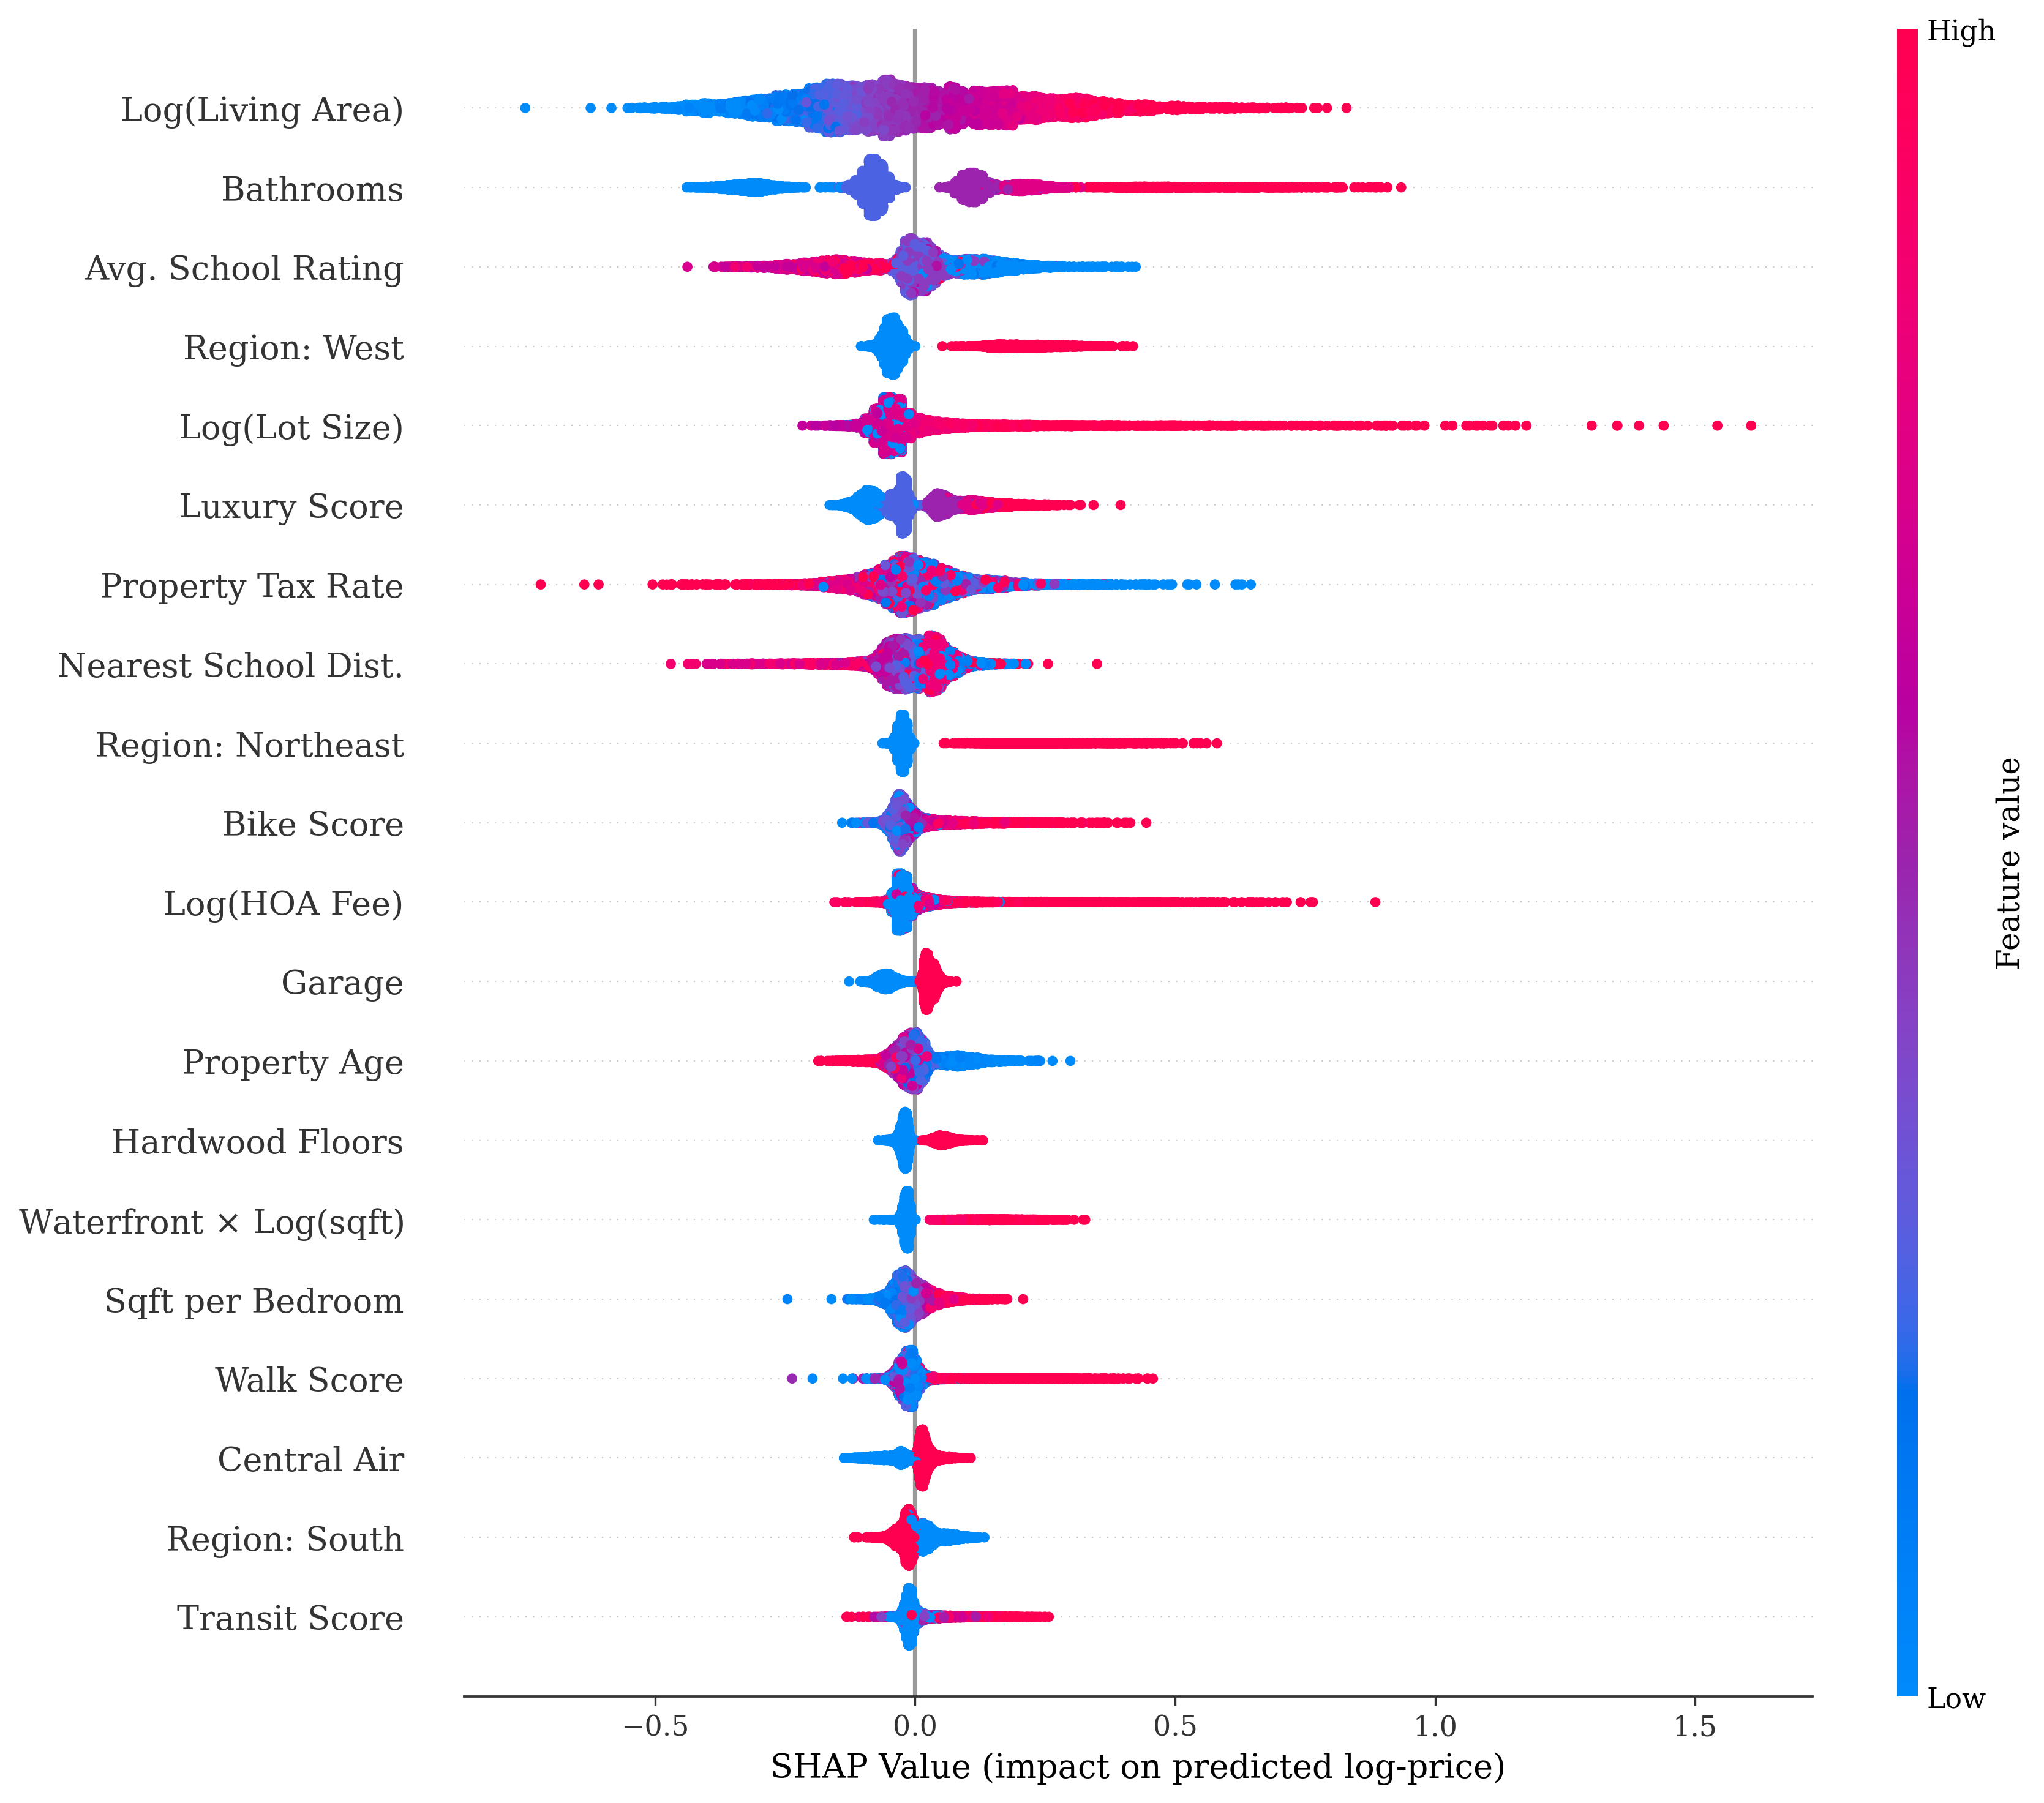
\includegraphics[width=0.85\textwidth]{figures/fig5_shap_summary.png}
    \caption{SHAP Summary Plot for XGBoost. Each dot is one observation; horizontal position shows the feature's SHAP value (contribution to predicted log-price deviation from the mean); color indicates feature value (red = high, blue = low). These are predictive contributions, not causal effects.}
    \label{fig:shap_summary}
\end{figure}

Living area and bathrooms are the two dominant predictive contributors, with mean absolute SHAP values of 0.174 and 0.161. School quality (0.088), regional location (West: 0.075; Northeast: 0.043), and lot size (0.075) form a second tier.

\textbf{SHAP dependence plots.} Figure~\ref{fig:shap_dependence} shows how the SHAP contribution of key features varies with feature values. The non-linear shapes---particularly the strongly concave living-area SHAP and the threshold-like behavior of school rating and property tax rate---explain why tree-based models outperform linear OLS. These non-linearities cannot be captured by the semi-log specification even with interaction terms.

\begin{figure}[H]
    \centering
    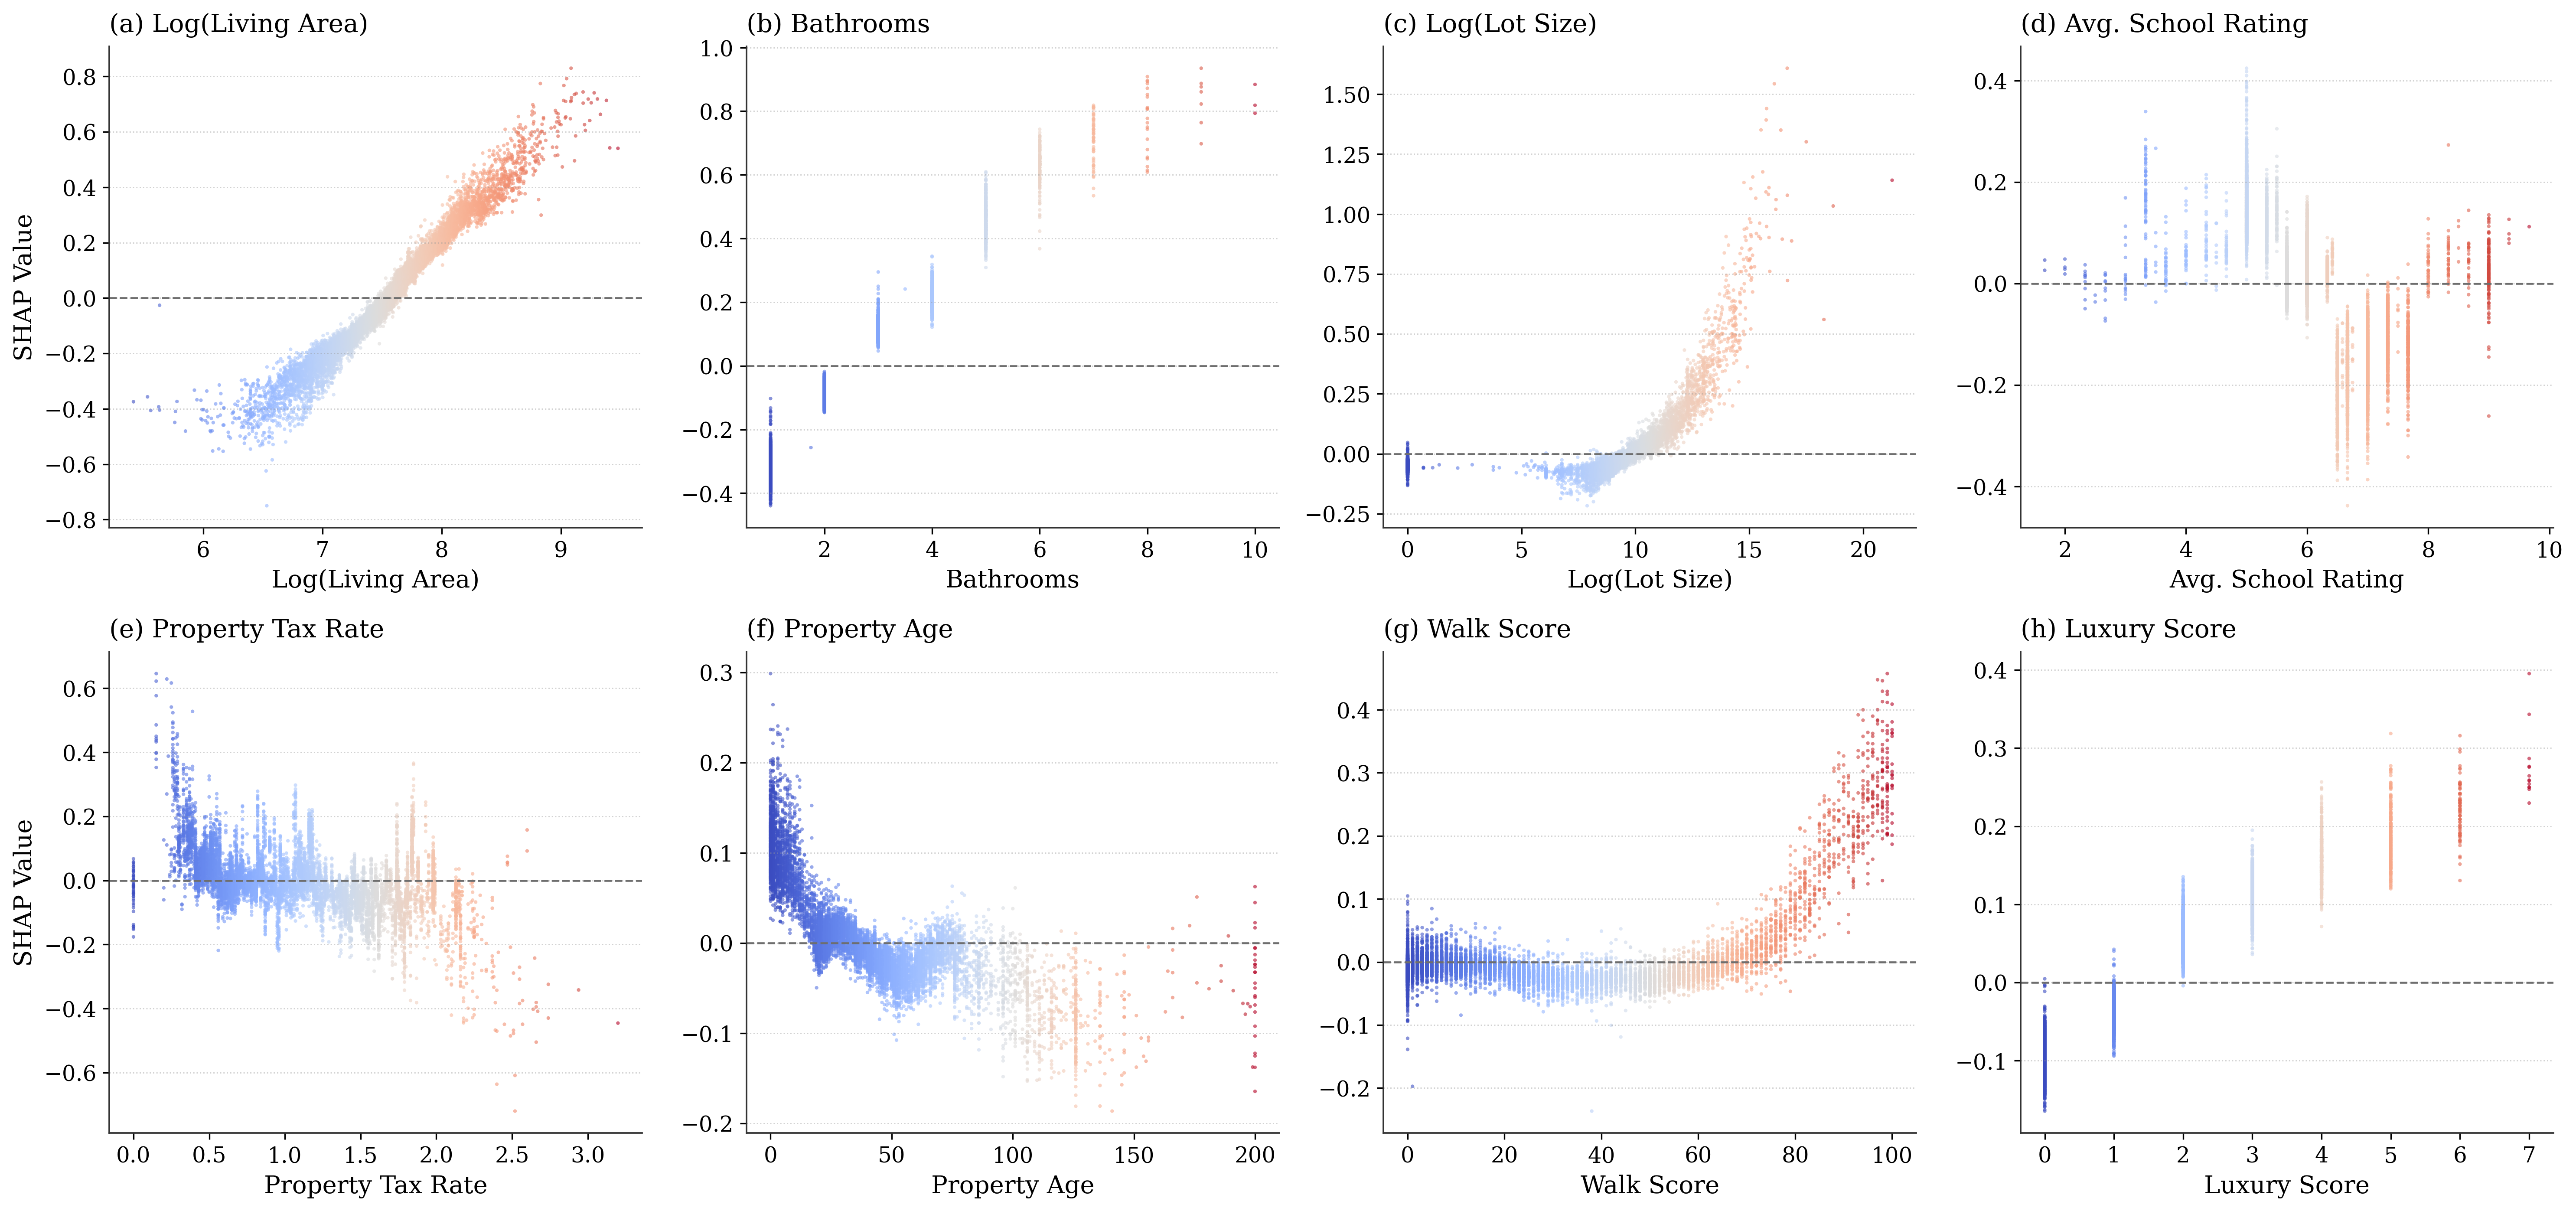
\includegraphics[width=\textwidth]{figures/fig10_shap_dependence.png}
    \caption{SHAP Dependence Plots for Eight Key Features. Each panel shows how the SHAP contribution varies with the feature value. Non-linear patterns (concavity, thresholds, saturation) explain the predictive advantage of tree-based models over linear specifications.}
    \label{fig:shap_dependence}
\end{figure}

\subsubsection{Cross-Model SHAP Stability}

A common concern with SHAP-based interpretation is that rankings may be model-specific artifacts. Table~\ref{tab:shap_stability} reports pairwise Spearman rank correlations of mean absolute SHAP values across three tree-based models.

\begin{table}[H]
\centering
\caption{Cross-Model SHAP Importance Stability: Spearman Rank Correlations}
\label{tab:shap_stability}
\begin{threeparttable}
\begin{tabular}{lrrr}
\toprule
& XGBoost & LightGBM & Random Forest \\
\midrule
XGBoost & 1.000 & 0.9898 & 0.9060 \\
LightGBM & 0.9898 & 1.000 & 0.8917 \\
Random Forest & 0.9060 & 0.8917 & 1.000 \\
\bottomrule
\end{tabular}
\begin{tablenotes}
\small
\item \textit{Notes:} Spearman $\rho$ computed on the full vector of mean $|\phi|$ values across all features. The same six features---$\ln$(Living Area), Bathrooms, Avg.\ School Rating, Region: West, $\ln$(Lot Size), and Luxury Score---rank in the top six across all three models.
\end{tablenotes}
\end{threeparttable}
\end{table}

The cross-model correlations are remarkably high. XGBoost and LightGBM produce nearly identical rankings ($\rho = 0.990$), while even the structurally different Random Forest model yields $\rho > 0.89$ with both gradient-boosted methods. The same six features appear in the top six across all three models. This stability lends credibility to the SHAP-based feature importance ranking as a description of the predictive structure of the data, not merely an artifact of a particular algorithm.

\textbf{Note on SHAP versus OLS comparisons.} SHAP importance rankings differ from both OLS $t$-statistics and XGBoost gain importance. School rating ranks 3rd by SHAP but has a counterintuitive negative OLS sign; property tax rate ranks 7th by SHAP but 28th by standardized OLS coefficient magnitude. These discrepancies reflect the non-linear and interactive effects that SHAP captures but OLS cannot. However, even though SHAP rankings are stable across tree-based models, they should not be interpreted as revealing the ``true'' importance hierarchy of housing attributes---they remain predictive decompositions, not structural parameters.


\subsection{Geographic Heterogeneity}

Figure~\ref{fig:geographic} maps the spatial distribution of listing prices. The well-documented coastal price gradient is clearly visible, with California, the Northeast corridor, Hawaii, and Colorado exhibiting the highest prices. The map also illustrates the non-representativeness concern: listing density is highly uneven, with sparse coverage in some rural areas.

\begin{figure}[H]
    \centering
    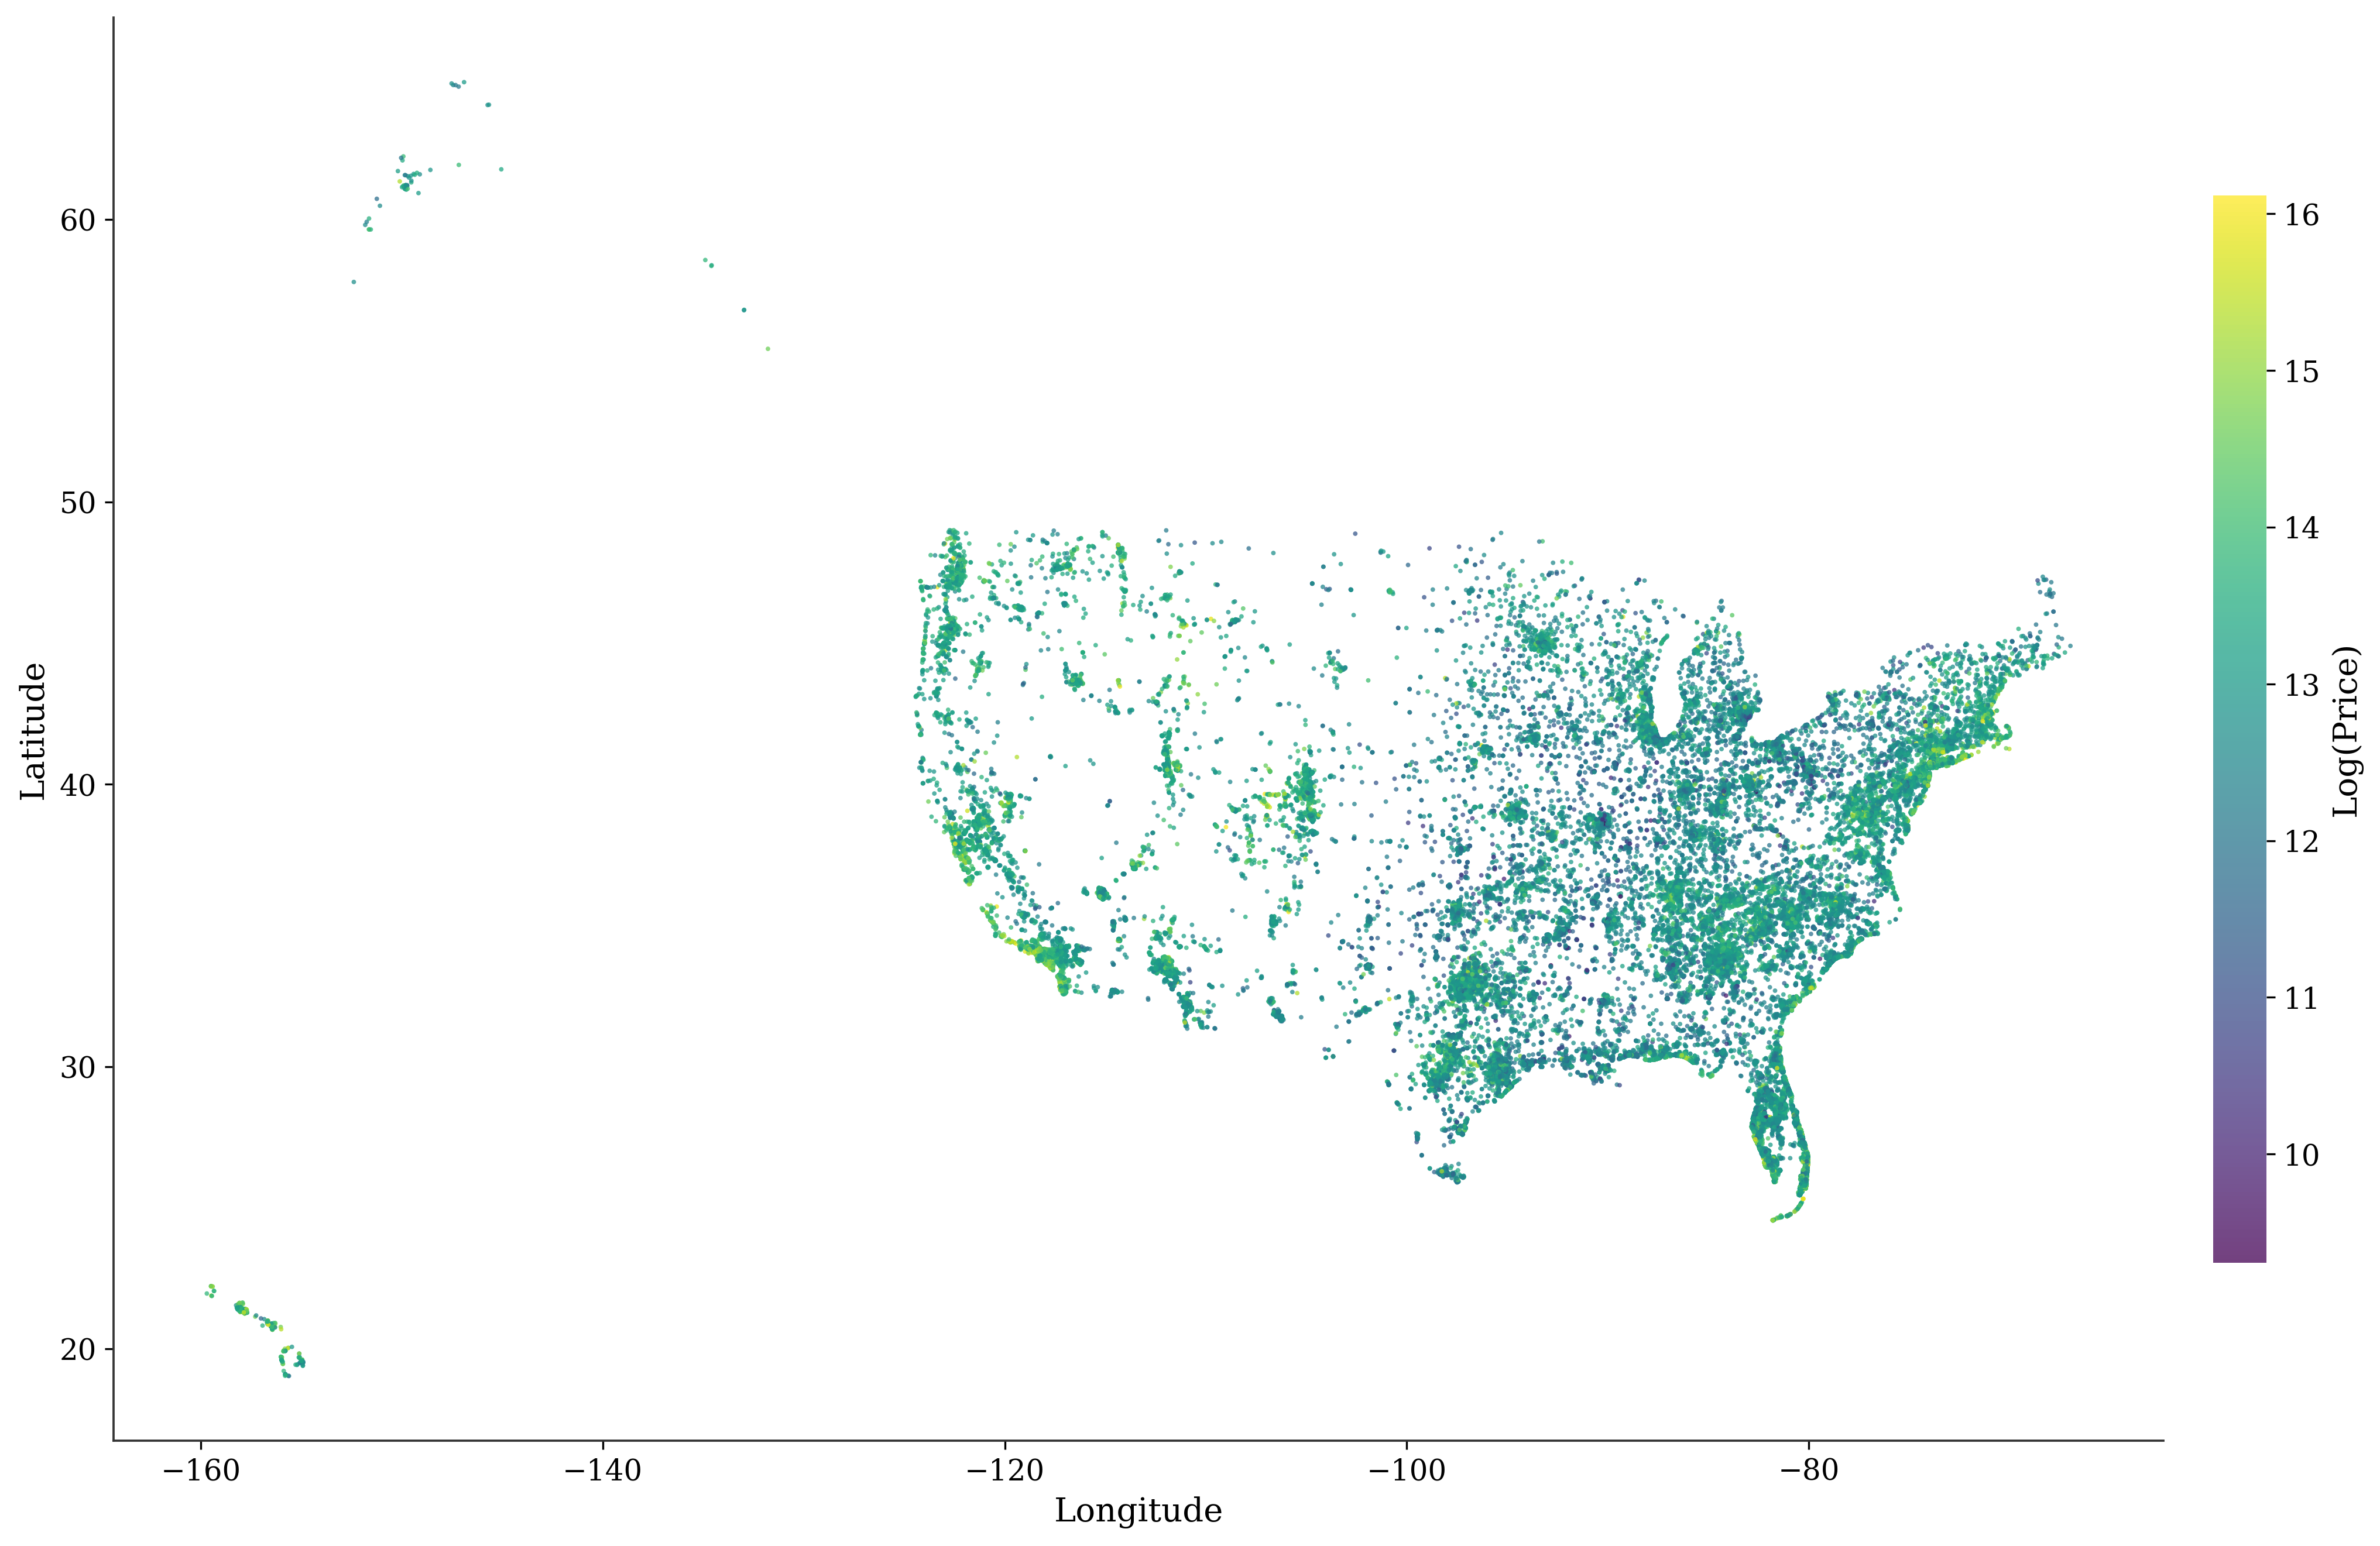
\includegraphics[width=\textwidth]{figures/fig7_geographic_prices.png}
    \caption{Geographic Distribution of Log Listing Prices. Each dot represents one property (50,000 random subsample). Color indicates log-price. Note: listing density is not uniform; areas with few dots may have fewer Zillow listings, not necessarily fewer properties.}
    \label{fig:geographic}
\end{figure}

\begin{figure}[H]
    \centering
    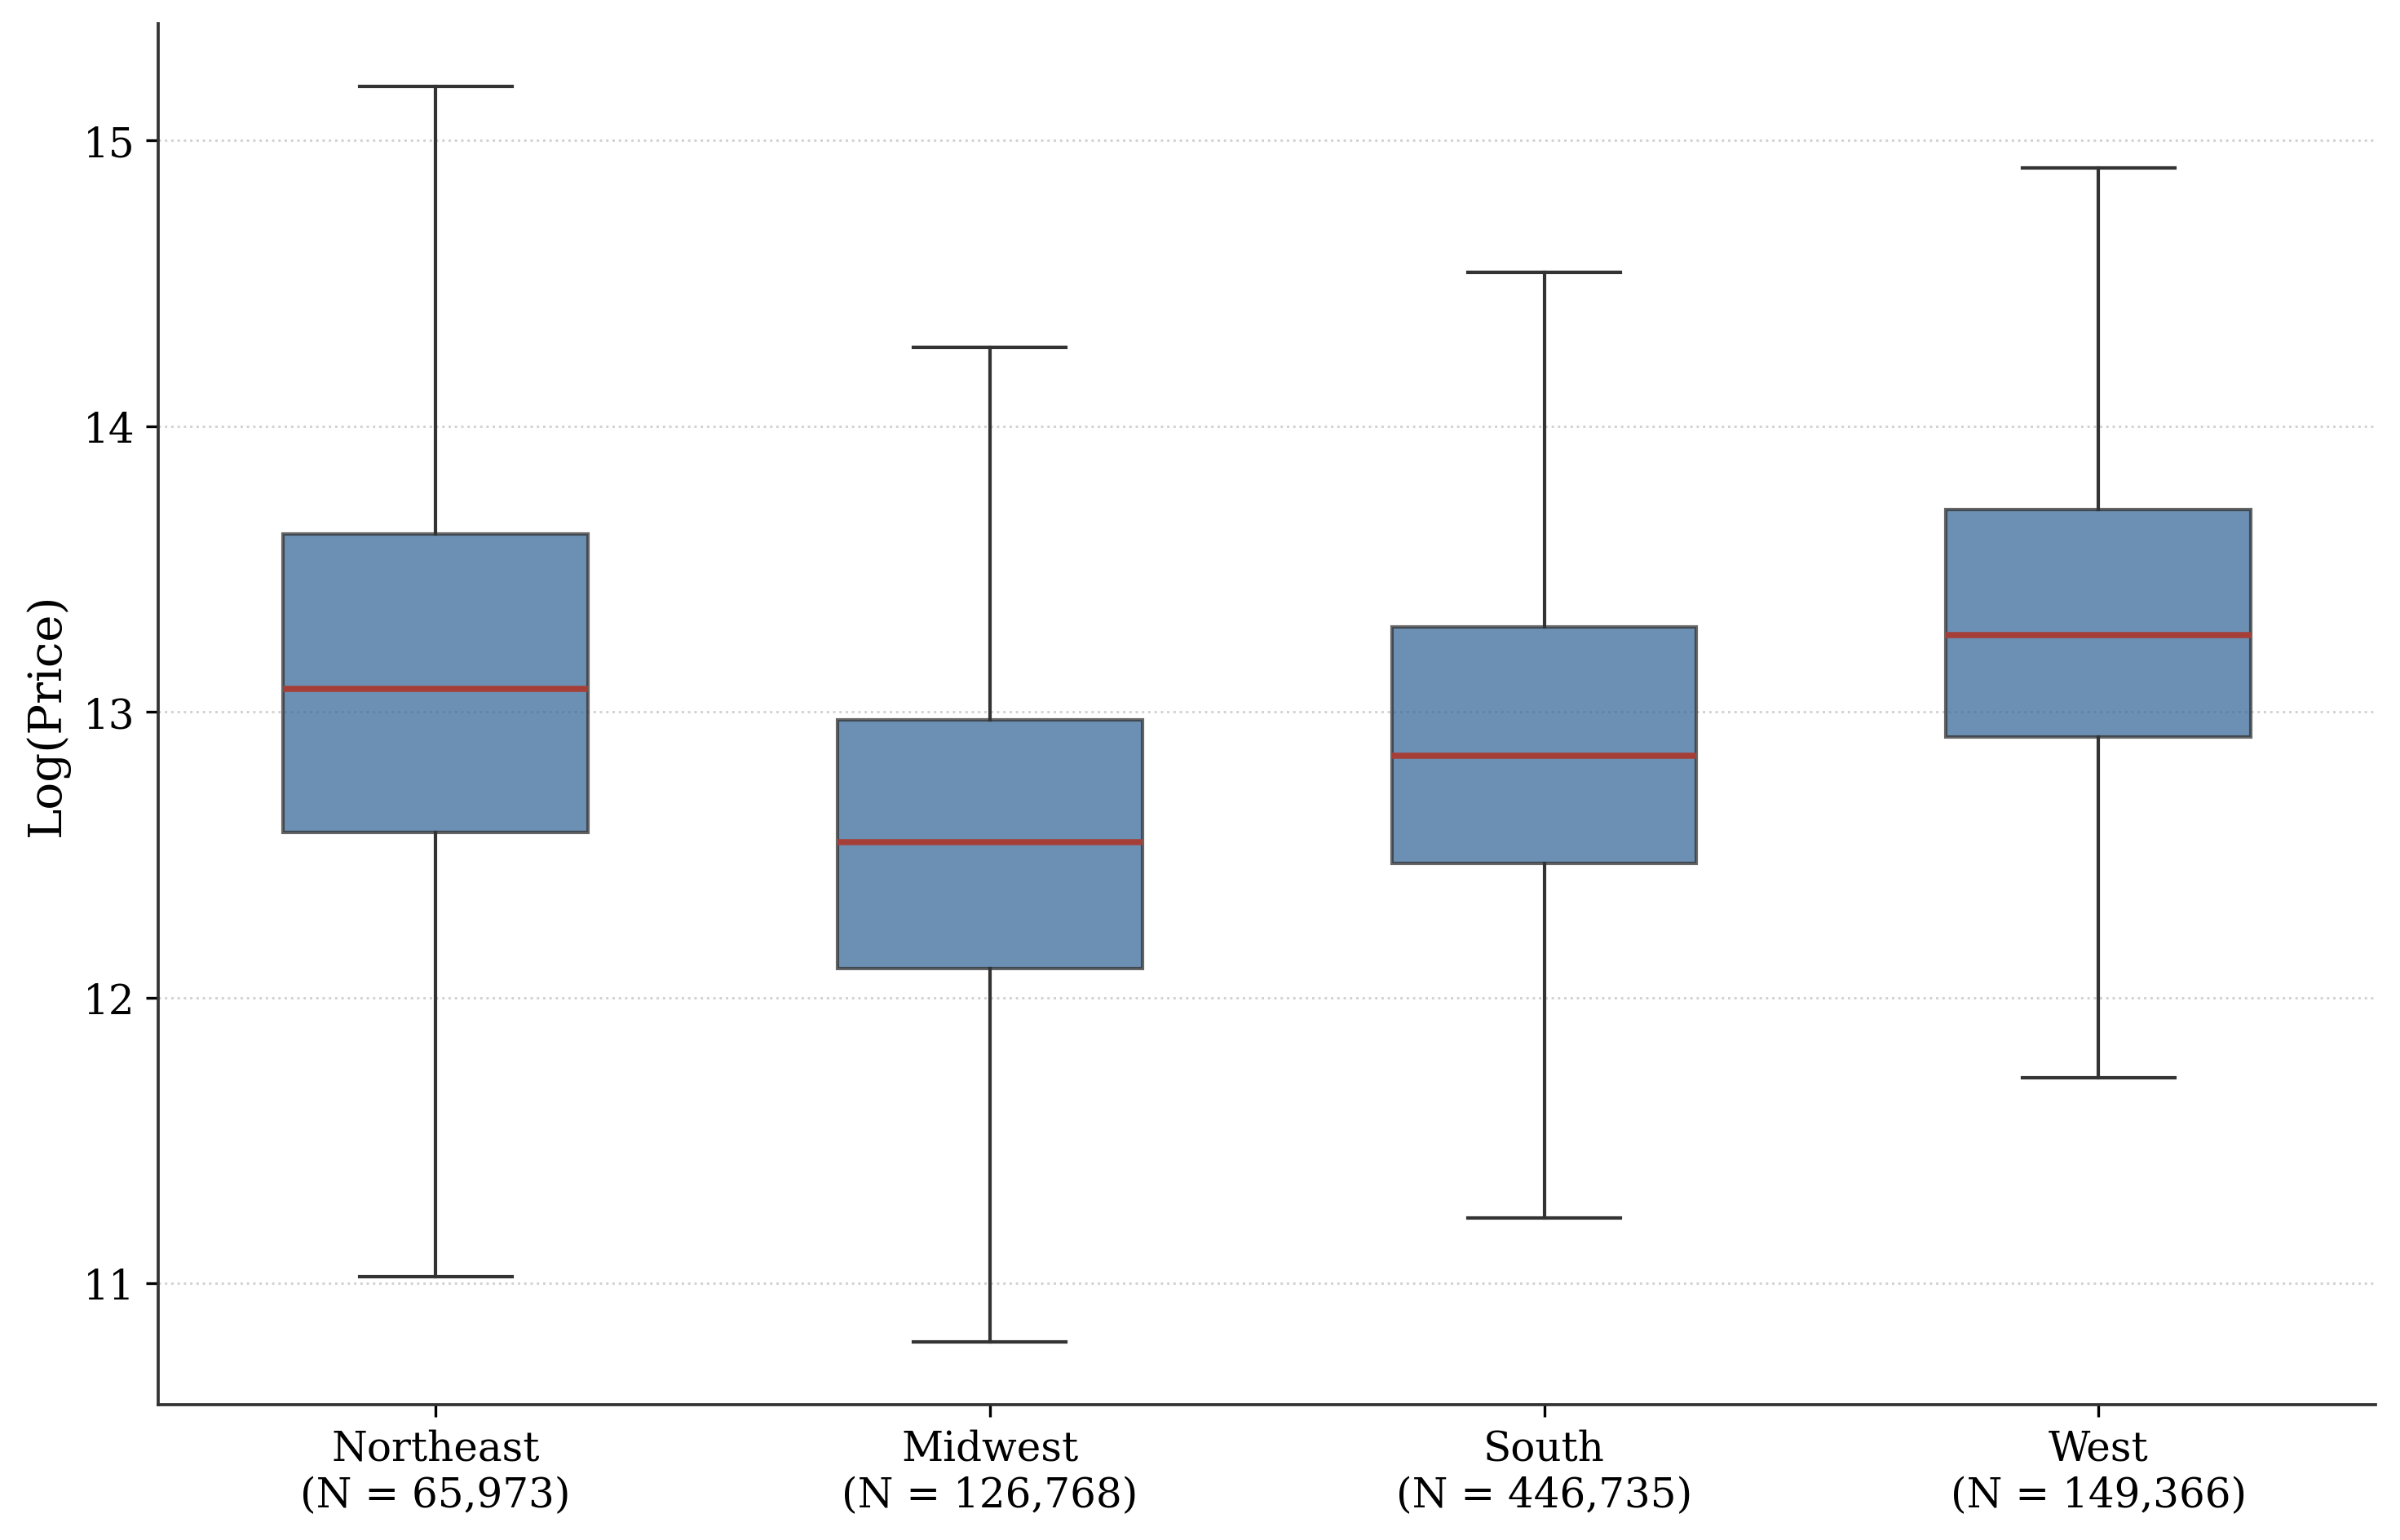
\includegraphics[width=0.85\textwidth]{figures/fig8_regional_prices.png}
    \caption{Listing Price Distribution by Census Region}
    \label{fig:regional}
\end{figure}


\subsection{Non-Linear Relationships}

Figure~\ref{fig:marginal} presents bivariate (unconditional) relationships between key attributes and log listing prices. These plots illustrate the non-linearities that motivate the machine learning approach but should not be confused with conditional (ceteris paribus) effects.

\begin{figure}[H]
    \centering
    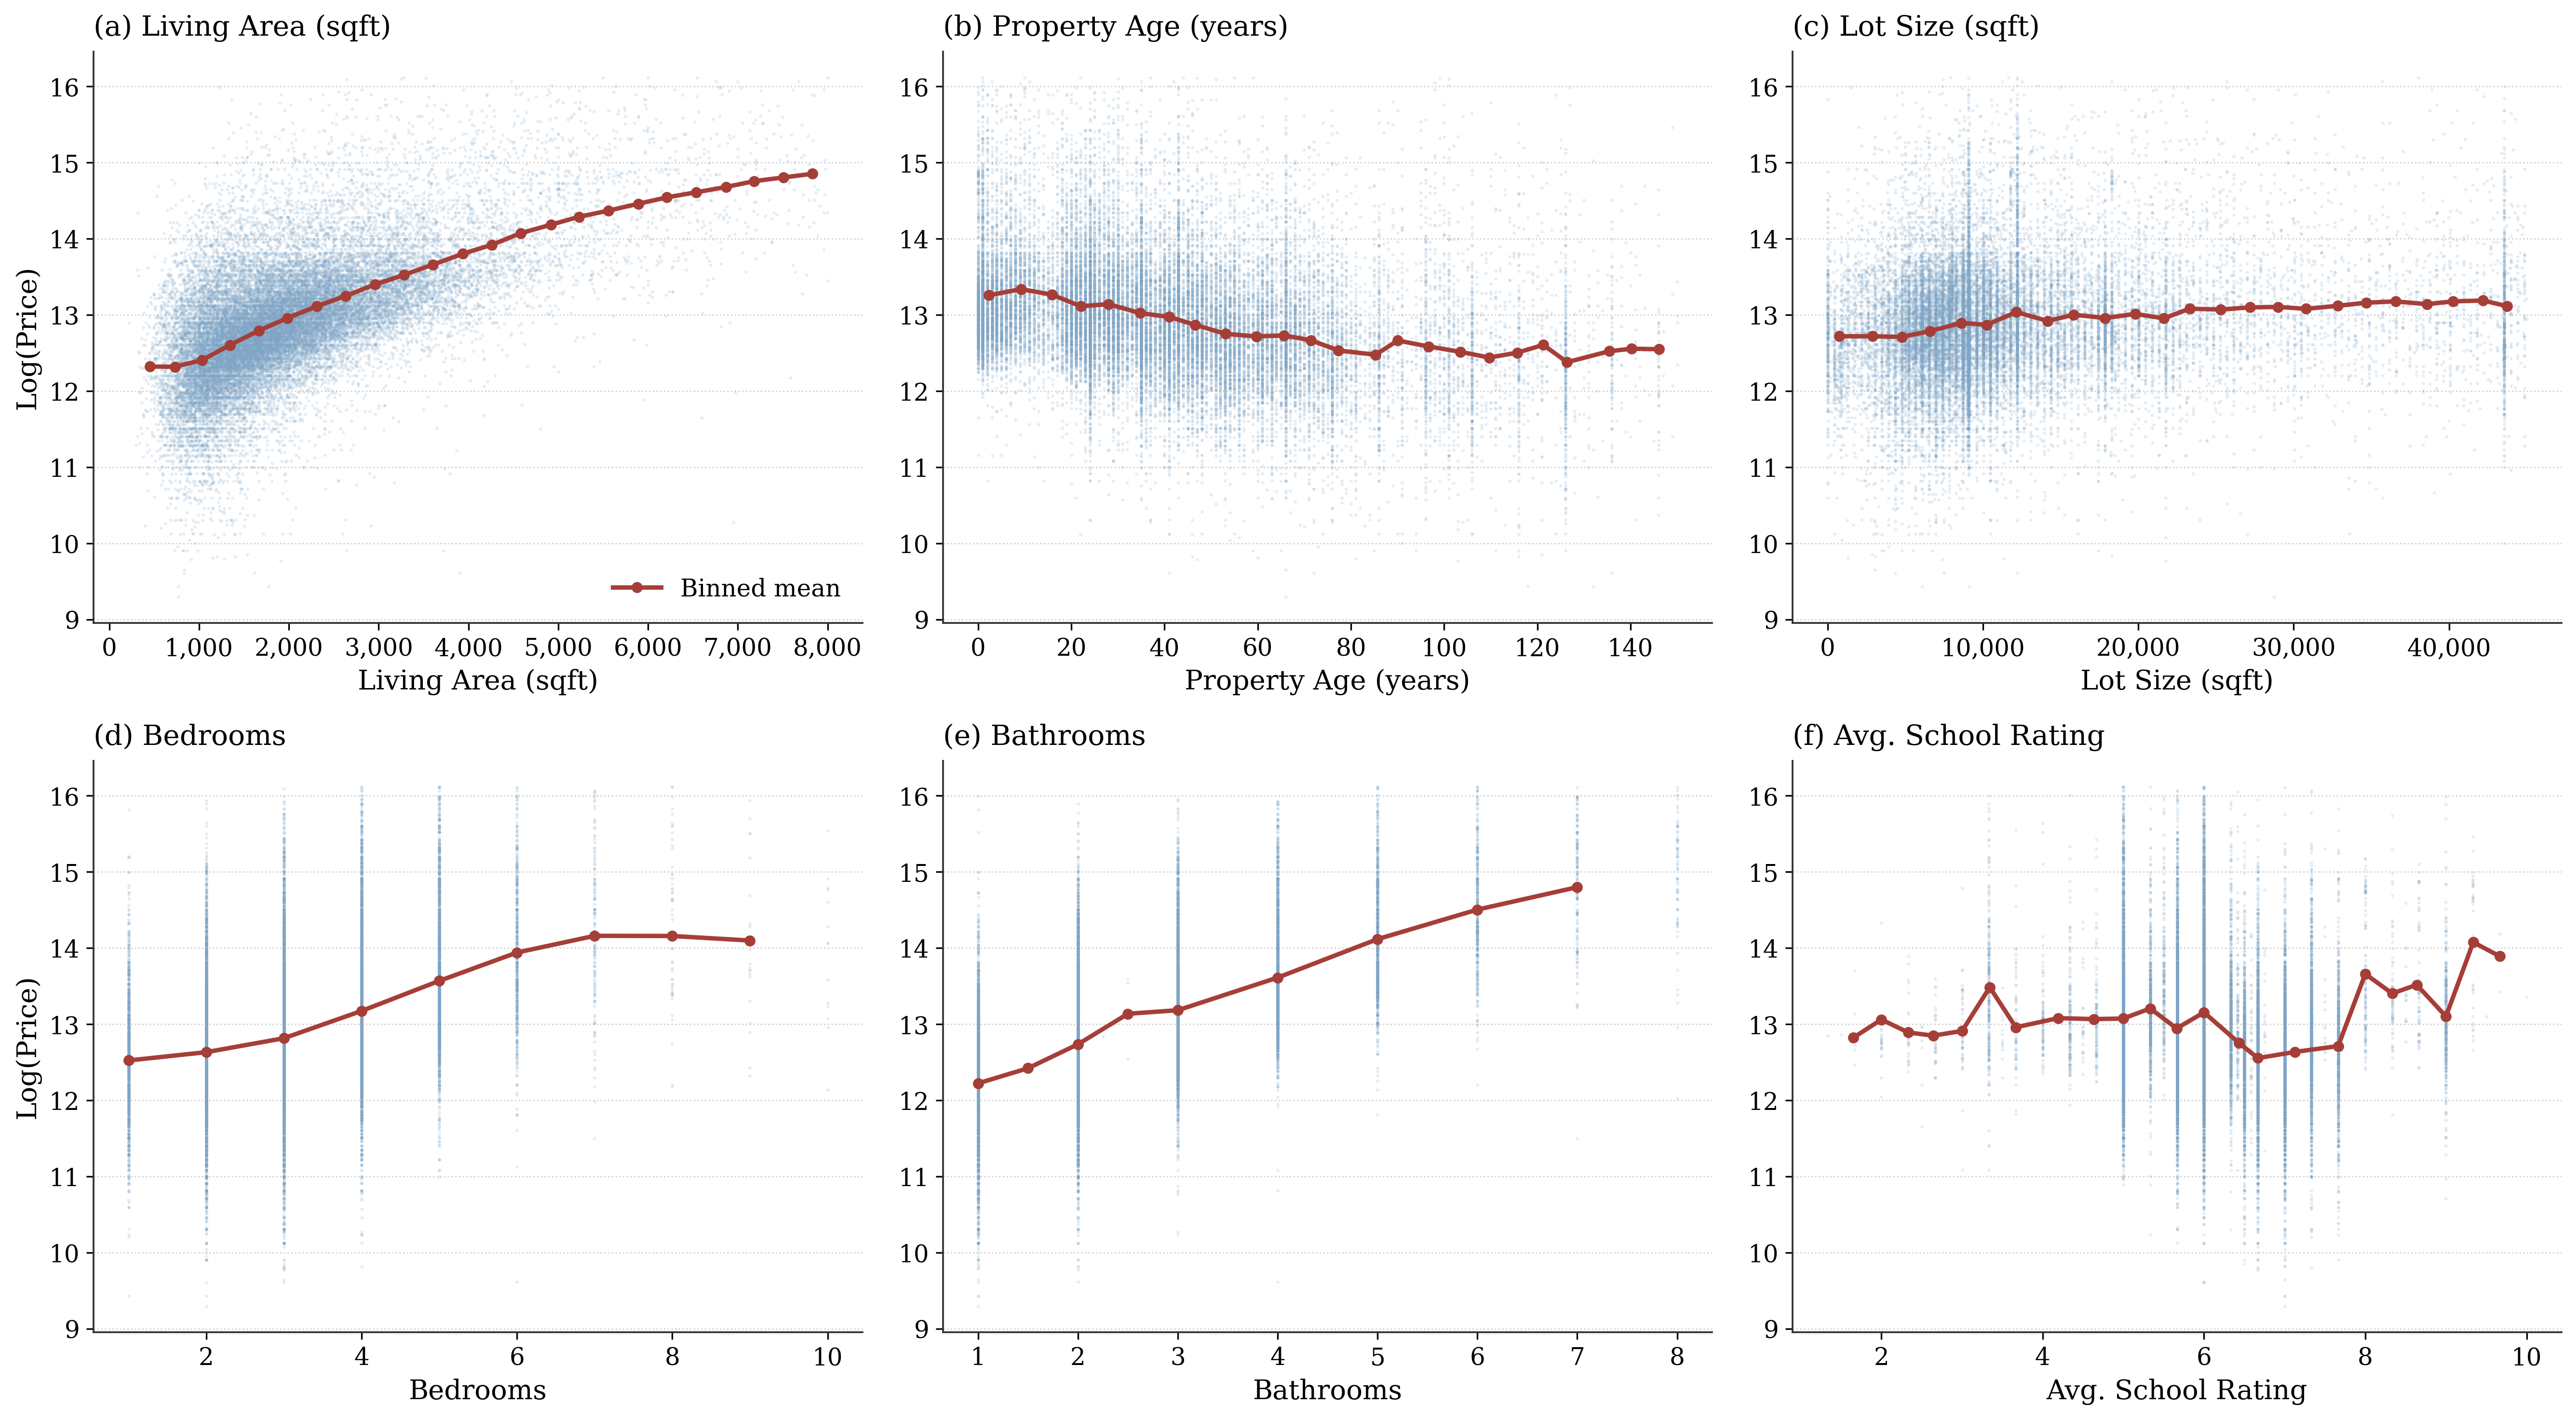
\includegraphics[width=\textwidth]{figures/fig9_marginal_effects.png}
    \caption{Unconditional Bivariate Relationships Between Key Attributes and Log Listing Price. These are raw scatter plots and binned means; they do not control for other attributes and should not be interpreted as conditional effects.}
    \label{fig:marginal}
\end{figure}

% Author: Simon-Pierre Boucher — contact@spboucher.ai
%
% ═══════════════════════════════════════════════════════════════════════
% 6. ROBUSTNESS
% ═══════════════════════════════════════════════════════════════════════
\section{Robustness Checks}
\label{sec:robustness}

\subsection{Imputation Sensitivity}
\label{sec:imputation_sensitivity}

Two variables with substantial missingness---year built (19.4\%) and lot size (16.3\%)---are imputed using state-level medians. To assess the consequences, we re-estimate the baseline OLS model on subsamples that exclude imputed observations. Table~\ref{tab:imputation} reports the results.

\begin{table}[H]
\centering
\caption{Imputation Sensitivity: Unstandardized OLS on Complete-Case Subsamples}
\label{tab:imputation}
\begin{threeparttable}
\small
\begin{tabular}{lrrrr}
\toprule
Specification & $N$ & $R^2$ & $\hat{\beta}_{\ln(\text{lot})}$ & Notes \\
\midrule
Full sample (baseline) & 788,842 & 0.634 & 0.018 & All imputed values included \\
Drop missing year\_built & 640,055 & 0.638 & 0.019 & 19\% fewer obs. \\
Drop missing lot\_size & 664,900 & 0.651 & 0.059 & 16\% fewer obs. \\
Drop both missing & 534,803 & 0.654 & 0.059 & 32\% fewer obs. \\
\bottomrule
\end{tabular}
\begin{tablenotes}
\small
\item \textit{Notes:} All specifications use the same 62-regressor unstandardized OLS model with HC3 standard errors. $\hat{\beta}_{\ln(\text{lot})}$ is the coefficient on $\ln$(lot size) in natural units. Other coefficients are broadly stable across specifications (not shown for brevity).
\end{tablenotes}
\end{threeparttable}
\end{table}

The key finding is that the \textbf{lot-size coefficient triples} from 0.018 to 0.059 when imputed lot sizes are dropped. This suggests that state-median imputation attenuates the lot-size gradient substantially: imputed properties receive the state median lot size regardless of their actual lot, washing out the true lot-price relationship. The $R^2$ also increases modestly ($+2.0$ pp) when imputed lots are excluded, indicating that imputation introduces noise.

Other coefficients (living area, bathrooms, age) are broadly stable across subsamples, suggesting that the imputation concern is primarily concentrated in the lot-size variable. Dropping observations with missing year built has minimal effect on the lot-size coefficient (0.018 to 0.019) and only slightly increases $R^2$ ($+0.4$ pp).

This sensitivity finding has implications for interpretation: the baseline elasticity of listing price with respect to lot size ($0.02$) likely understates the true association, and the complete-case estimate ($0.06$) may be more informative---though it applies to a selected (non-randomly missing) subsample.


\subsection{Winsorization Sensitivity}
\label{sec:winsorization}

To assess the influence of outliers, we winsorize the two variables with implausible extreme values---lot size, capped at its 99.5th percentile (3,944 observations affected), and Bike Score, capped at its nominal maximum of 100 (38 observations)---and re-estimate the baseline OLS model.

\begin{table}[H]
\centering
\caption{Winsorization Sensitivity: Baseline vs.\ Winsorized OLS}
\label{tab:winsorization}
\begin{threeparttable}
\small
\begin{tabular}{lrr}
\toprule
Metric / Coefficient & Baseline & Winsorized \\
\midrule
$R^2$ & 0.634 & 0.640 \\
$\hat{\beta}_{\ln(\text{lot})}$ & 0.018 & 0.058 \\
$\hat{\beta}_{\ln(\text{sqft})}$ & 0.628 & 0.610 \\
$\hat{\beta}_{\text{bathrooms}}$ & 0.204 & 0.211 \\
$\hat{\beta}_{\text{garage}}$ & 0.109 & 0.111 \\
\bottomrule
\end{tabular}
\begin{tablenotes}
\small
\item \textit{Notes:} Lot size winsorized at its 99.5th percentile ($\approx 3.04$ million sqft; 3,944 observations capped); Bike Score capped at 100 (38 observations). Unstandardized OLS, $N = 788{,}842$. Other coefficients broadly stable (not shown). The large change in $\hat{\beta}_{\ln(\text{lot})}$ mirrors the imputation sensitivity finding, likely reflecting outlier lot sizes in imputed observations.
\end{tablenotes}
\end{threeparttable}
\end{table}

Winsorization increases $R^2$ modestly from 0.634 to 0.640, suggesting that extreme values in continuous variables account for a small portion of unexplained variation. The lot-size coefficient again jumps substantially (0.018 to 0.058), consistent with the imputation sensitivity analysis: extreme imputed lot sizes attenuate the gradient. Other coefficients are broadly stable, indicating that the main OLS results are not driven by outliers.


\subsection{Quantile Regression Subsample Stability}
\label{sec:qr_stability}

We repeat the median quantile regression ($\tau = 0.50$) across 10 random subsamples of 150,000 observations each. Table~\ref{tab:qr_stability} reports the coefficient of variation (CV) and sign stability for key variables.

\begin{table}[H]
\centering
\caption{Quantile Regression Stability: $\tau = 0.50$ Across 10 Subsamples}
\label{tab:qr_stability}
\begin{threeparttable}
\small
\begin{tabular}{lrrl}
\toprule
Variable & CV (\%) & Sign Stability (\%) & Assessment \\
\midrule
West & 1.0 & 100 & Highly stable \\
Northeast & 1.6 & 100 & Highly stable \\
$\ln$(Lot Size) & 2.7 & 100 & Highly stable \\
$\ln$(Living Area) & 2.9 & 100 & Highly stable \\
Bathrooms & 2.9 & 100 & Highly stable \\
Garage & 4.1 & 100 & Highly stable \\
Luxury Score & 4.8 & 100 & Highly stable \\
Age$^2$ & 5.3 & 100 & Highly stable \\
Foreclosure & 7.1 & 100 & Stable \\
Bedrooms & 7.3 & 100 & Stable \\
\midrule
\multicolumn{4}{l}{\textit{Less stable variables}} \\
Pool & 33.4 & 100 & Moderately unstable \\
Waterfront & 42.2 & 100 & Moderately unstable \\
Age & 78.6 & 80 & Unstable \\
\bottomrule
\end{tabular}
\begin{tablenotes}
\small
\item \textit{Notes:} CV = coefficient of variation across 10 random subsamples of 150,000 observations. Sign stability = percentage of subsamples in which the coefficient has the same sign as the pooled estimate. Variables sorted by CV. The instability of age (CV = 78.6\%) likely reflects heterogeneity in the age-price relationship across geographic subsamples. The waterfront and pool coefficients vary in magnitude but never change sign; their instability reflects low variation in these binary variables in some subsamples.
\end{tablenotes}
\end{threeparttable}
\end{table}

Most variables exhibit high stability (CV $< 8\%$, 100\% sign stability), confirming that the quantile regression results are robust to subsample variation. Three variables are exceptions: \textbf{age} (CV = 78.6\%, sign stability = 80\%), \textbf{waterfront} (CV = 42.2\%), and \textbf{pool} (CV = 33.4\%). The instability of age is consistent with substantial geographic heterogeneity in the age-price relationship---old properties may command a premium in some markets (historic charm) and a discount in others (obsolescence). Waterfront and pool instability reflects the relatively low prevalence of these features in some subsamples.


\subsection{Robustness Summary Matrix}
\label{sec:robustness_matrix}

Table~\ref{tab:robustness_matrix} provides a comprehensive summary of all robustness findings.

\begin{table}[H]
\centering
\caption{Robustness Summary Matrix}
\label{tab:robustness_matrix}
\begin{threeparttable}
\footnotesize
\begin{tabular}{p{3.5cm}p{2.5cm}p{2.5cm}p{4.5cm}}
\toprule
Test & Baseline & Robustness & Key Finding \\
\midrule
\multicolumn{4}{l}{\textit{OLS Specification}} \\
Region FE $\rightarrow$ State FE & $R^2 = 0.630$ & $R^2 = 0.678$ & $+$4.8 pp from state-level controls \\
Region FE $\rightarrow$ ZIP3 FE & $R^2 = 0.630$ & $R^2 = 0.725$ & $+$9.5 pp from ZIP3 controls \\
Drop imputed lot sizes & $\hat{\beta}_{\ln\text{lot}} = 0.018$ & $\hat{\beta}_{\ln\text{lot}} = 0.059$ & Coefficient triples; imputation attenuates \\
Winsorization (1\%/99\%) & $R^2 = 0.634$ & $R^2 = 0.640$ & Modest improvement; lot coeff.\ sensitive \\
\midrule
\multicolumn{4}{l}{\textit{Spatial Diagnostics}} \\
Moran's $I$ (3 subsamples) & $I = 0.2745$ & std $= 0.0076$ & Highly stable; strong spatial autocorrelation \\
\midrule
\multicolumn{4}{l}{\textit{Quantile Regression}} \\
QR stability (10 draws) & Most CV $< 8\%$ & Age CV = 78.6\% & Age unstable; all others sign-stable \\
Inter-quantile Wald & --- & 11/13 significant & Distribution varies for most attributes \\
\midrule
\multicolumn{4}{l}{\textit{Machine Learning}} \\
Random vs.\ geo holdout & $R^2 = 0.833$ & $R^2 = 0.425$ & 40.8 pp gap; spatial leakage \\
Remove geo features & Geo $R^2 = 0.425$ & Geo $R^2 = 0.519$ & $+$9.4 pp; geography hurts generalization \\
Add lat/lon & Random $R^2 = 0.870$ & Geo $R^2 = 0.464$ & Coordinates memorize location \\
Ablation: neighborhood & --- & $+$17.6 pp random & Largest single feature-group contribution \\
Ablation: full model & --- & $-$7.6 pp geo & Region dummies harm generalization \\
\midrule
\multicolumn{4}{l}{\textit{SHAP Stability}} \\
XGBoost vs.\ LightGBM & --- & $\rho = 0.990$ & Near-identical rankings \\
XGBoost vs.\ RF & --- & $\rho = 0.906$ & Consistent top-6 features \\
LightGBM vs.\ RF & --- & $\rho = 0.892$ & Consistent top-6 features \\
\bottomrule
\end{tabular}
\begin{tablenotes}
\footnotesize
\item \textit{Notes:} This table summarizes all robustness checks conducted in the paper. ``pp'' = percentage points. All findings refer to the same base sample of $N = 788{,}842$ unless noted. The geographic holdout $R^2$ of 0.425 for the full XGBoost model reflects the variant with region dummies included in the ablation design; the main specification yields 0.547 due to differences in training-set composition.
\end{tablenotes}
\end{threeparttable}
\end{table}

% Author: Simon-Pierre Boucher — contact@spboucher.ai
%
% ═══════════════════════════════════════════════════════════════════════
% 7. DISCUSSION
% ═══════════════════════════════════════════════════════════════════════
\section{Discussion}
\label{sec:discussion}

The results support four main messages, each associated with a specific modeling framework.

\subsection{Message 1: OLS Remains Useful for Interpretable Associations}

The semi-log OLS model explains 63.4\% of the variation in log listing prices using 62 regressors, comparable to the typical hedonic $R^2$ in the literature \citep{sirmans2005composition}. Its primary value lies in interpretability: the coefficients provide conditional mean associations in a transparent functional form. Regularized linear models (Ridge, Lasso, Elastic Net) achieve essentially identical performance ($R^2 = 0.628$--$0.630$), confirming that the OLS specification is not overfit and that the 20-percentage-point gap relative to XGBoost reflects genuine non-linearities and interactions, not parametric overfitting.

The progression from region FE ($R^2 = 0.634$) to state FE ($0.678$) to ZIP3 FE ($0.725$) reveals that a large portion of the unexplained variation is spatial in nature. The ZIP3 FE model closes roughly half the gap between baseline OLS and XGBoost, suggesting that fine-grained geographic controls---rather than non-linear functional forms---account for much of the ML advantage. However, ZIP3 FE introduces 886 parameters and sacrifices the parsimony that makes OLS attractive for economic interpretation.

The imputation sensitivity analysis reveals that the baseline lot-size elasticity (0.02) is substantially attenuated by state-median imputation; the complete-case estimate (0.06) is more plausible but applies to a selected subsample. This finding underscores the importance of data quality audits in hedonic research.

\subsection{Message 2: Quantile Regression Adds Distributional Insight}

Quantile regression reveals that OLS coefficients mask substantial distributional heterogeneity. The garage gradient ratio (10.3:1 between $\tau = 0.10$ and $\tau = 0.90$) and the pool gradient reversal (insignificant at lower quantiles, strongly positive at upper quantiles) demonstrate that the same attribute can play fundamentally different roles across market segments. Inter-quantile Wald tests confirm that these differences are statistically significant for 11 of 13 tested variables, with garage ($z = 28.92$) being the most significantly heterogeneous.

This has implications for housing policy: interventions that improve basic amenities (garages, heating systems) may generate the largest listing-price differentials at the lower end, while luxury amenity provision primarily differentiates upper-market properties.

The subsample stability analysis shows that most quantile coefficients are highly robust (CV $< 8\%$), but age stands out as unstable (CV = 78.6\%, sign stability = 80\%), reflecting genuine geographic heterogeneity in how property age relates to listing prices.

\subsection{Message 3: ML Performance Depends Critically on Validation Design}

The XGBoost model achieves substantially better predictions than OLS under random validation ($R^2 = 0.833$ vs.\ $0.630$), capturing non-linearities and interactions that the parametric specification cannot. However, the geographic holdout results provide an important corrective: under state-level holdout, XGBoost achieves only $R^2 = 0.425$--$0.547$ depending on specification.

The ablation analysis pinpoints what drives the ML gain. Neighborhood features contribute $+17.6$ pp in random $R^2$---the largest single gain---but only $+3.5$ pp in geographic holdout $R^2$. This disparity suggests that neighborhood variables (school ratings, Walk Score, etc.) are highly informative within observed markets but carry location-specific scale and meaning that may not transfer. The full model with region dummies actually \emph{reduces} geographic holdout $R^2$ by 7.6 pp relative to the market-status-only specification.

The most striking finding is that removing all geographic features \emph{improves} geographic holdout $R^2$ from 0.425 to 0.519. This is the opposite of what intuition might suggest and has direct implications for AVM deployment: in contexts requiring geographic generalization, simpler models without explicit geography may outperform richer ones.

\subsection{Message 4: SHAP Interprets Prediction, Not Economics}

SHAP values provide useful prediction-level decompositions that identify which features drive the XGBoost model's predictions for individual properties. The cross-model stability analysis ($\rho = 0.89$--$0.99$ across three tree models) addresses the common criticism that SHAP rankings are model-specific: while individual SHAP values differ, the ranking of feature importance is remarkably consistent, with the same six features dominating all three models.

However, SHAP values should not be equated with hedonic listing-price gradients:
\begin{itemize}[nosep]
    \item SHAP values decompose predictions, not the data-generating process. A feature with a large SHAP value may be predictively important because it proxies for unobserved variables, not because it has a large association with listing prices in the structural sense.
    \item Feature correlation distributes SHAP contributions among correlated features in ways that may not reflect economic importance.
    \item SHAP importance rankings differ from OLS coefficient rankings (e.g., school rating ranks 3rd by SHAP but has a counterintuitive negative OLS sign), reflecting the different questions each framework answers.
\end{itemize}

In the terminology of \citet{mullainathan2017machine}, SHAP is a tool for interpreting predictions. The hedonic gradient $\partial P / \partial z_k$ is a tool for understanding market structure. These serve different purposes and should not be conflated.

% Author: Simon-Pierre Boucher — contact@spboucher.ai
%
% ═══════════════════════════════════════════════════════════════════════
% 8. LIMITATIONS
% ═══════════════════════════════════════════════════════════════════════
\section{Limitations}
\label{sec:limitations}

We summarize the principal limitations in a structured format.

\begin{enumerate}[nosep]
    \item \textbf{Listing prices, not transaction prices.} The dependent variable is the asking price, which may differ from the realized sale price due to strategic pricing, negotiation, and market conditions. Listing-price gradients are not necessarily equivalent to transaction-price implicit prices.

    \item \textbf{No causal identification.} All estimates are conditional associations. Without exogenous variation, we cannot distinguish the causal effects of attributes from sorting, supply constraints, and omitted variables \citep{ekeland2004identification, roberts2013endogeneity}.

    \item \textbf{Spatial dependence not modeled.} Moran's $I = 0.27$ confirms substantial spatial autocorrelation in OLS residuals. The paper does not estimate spatial lag, spatial error, or geographically weighted regression models, which may affect both efficiency and consistency of estimates.

    \item \textbf{Random validation overstates ML performance.} The random train-test split allows spatial leakage. Under geographic holdout, XGBoost $R^2$ drops from 0.833 to 0.425--0.547 depending on specification.

    \item \textbf{Standardization complicates interpretation.} The standardized OLS coefficients are not directly interpretable as elasticities or semi-elasticities. We provide an unstandardized specification for economic interpretation but note that some readers may conflate the two.

    \item \textbf{Missing data and imputation.} Year built (19.4\%), lot size (16.3\%), and transit score (70.1\%) have substantial missingness. State-median imputation preserves geographic variation but attenuates the lot-size coefficient by a factor of three.

    \item \textbf{Climate risk variables entirely missing.} Despite their growing importance, flood, fire, heat, wind, and air risk factors could not be incorporated \citep{baldauf2020does}.

    \item \textbf{SHAP values are not structural implicit prices.} SHAP provides prediction decompositions, not marginal willingness-to-pay estimates. Cross-model stability supports the ranking but not the economic interpretation.

    \item \textbf{Quantile regression subsample.} Quantile regression is estimated on 150,000 observations (19\% of the full sample) for computational reasons. Most coefficients are stable (CV $< 8\%$) but age is not (CV = 78.6\%).

    \item \textbf{Non-representative sample.} The Zillow listing dataset overrepresents Southern states, active listings, and possibly certain property types. Results may not generalize to the full U.S.\ housing stock.

    \item \textbf{Data quality concerns.} Bike Score exceeds 100 for 38 observations; some lot sizes are implausibly large; parking-space data are noisy. These affect a small fraction of observations but may influence tail estimates.

    \item \textbf{No hyperparameter tuning via cross-validation.} XGBoost and LightGBM hyperparameters were set based on common defaults rather than optimized via nested cross-validation. Performance could potentially improve with systematic tuning.

    \item \textbf{Geographic holdout design is conservative.} Holding out 10 entire states is a stringent test; finer geographic blocking (county-level or MSA-level) might yield intermediate performance estimates that are more relevant for some AVM applications.

    \item \textbf{Single cross-section.} The data represent a snapshot of active listings at one point in time. Temporal variation in hedonic gradients---due to market cycles, interest rate changes, or policy shifts---cannot be examined.
\end{enumerate}

% Author: Simon-Pierre Boucher — contact@spboucher.ai
%
% ═══════════════════════════════════════════════════════════════════════
% 9. CONCLUSION
% ═══════════════════════════════════════════════════════════════════════
\section{Conclusion}
\label{sec:conclusion}

This paper has compared three approaches to hedonic housing price analysis---OLS, quantile regression, and gradient-boosted machine learning with SHAP interpretation---using a large Zillow listing sample of 788,842 U.S.\ properties. Each framework answers a different question, and the robustness extensions in this version document the boundaries of each framework's conclusions.

OLS provides interpretable conditional mean associations: a price-to-area elasticity of 0.63, a 22.6\% bathroom listing-price gradient, a 33.4\% foreclosure discount, and regional listing-price differentials of 49\%--63\% between coastal and interior markets. The progression from region FE ($R^2 = 0.634$) to ZIP3 FE ($R^2 = 0.725$) demonstrates that fine-grained geographic controls capture substantial variation, but the imputation sensitivity analysis reveals that the lot-size gradient is attenuated threefold by state-median imputation.

Quantile regression reveals that mean effects mask substantial distributional heterogeneity, now formally confirmed by inter-quantile Wald tests that reject coefficient equality for 11 of 13 variables. The garage listing-price gradient is ten times larger at the 10th percentile than the 90th ($z = 28.92$); the pool gradient is insignificant below the median but reaches 9.9\% at $\tau = 0.90$. Subsample stability analysis identifies age as the one coefficient that is genuinely unstable across geographic subsamples.

XGBoost captures non-linearities and interactions that improve prediction from $R^2 = 0.630$ (OLS) to $R^2 = 0.833$ under random validation. However, this figure substantially overstates generalization ability. The ablation analysis reveals that neighborhood features drive the largest predictive gain ($+17.6$ pp) but that the full model with region dummies actively harms geographic holdout ($-7.6$ pp). The most striking result is that removing all geographic features \emph{improves} geographic holdout $R^2$ from 0.425 to 0.519, while adding latitude and longitude does the opposite ($+3.7$ pp random, $-5.5$ pp geographic). Geographic features help the model memorize location-specific prices but do not improve its ability to generalize attribute-price relationships to new markets.

SHAP values identify the features that contribute most to predictions---living area, bathrooms, school quality, lot size, region---and this ranking is stable across three tree-based models (Spearman $\rho = 0.89$--$0.99$). But these remain predictive decompositions, not structural listing-price gradients. Moran's $I = 0.27$ on OLS residuals---stable across three subsamples (std $= 0.008$)---confirms that regional controls leave substantial spatial dependence unaddressed.

The central contribution is methodological: we demonstrate that model evaluation depends critically on validation design. Random splits overstate generalization, geographic features can harm geographic holdout, SHAP values are stable across models but remain non-structural, and imputation can attenuate key coefficients. Future research should integrate spatial econometric methods, use transaction prices, employ geographic holdout validation as standard practice, incorporate climate risk data, and benchmark against generalized additive models to decompose the ML predictive gain into non-linearity versus spatial partitioning components.

The central lesson is not that machine learning replaces hedonic econometrics, but that prediction, distributional heterogeneity, and economic interpretation answer different questions and should be combined carefully in modern housing valuation research.


% --- References ---
\newpage
\addcontentsline{toc}{section}{References}
\bibliography{references}

% --- Appendix ---
\newpage
% Author: Simon-Pierre Boucher — contact@spboucher.ai
%
% ═══════════════════════════════════════════════════════════════════════
% APPENDICES
% ═══════════════════════════════════════════════════════════════════════
\appendix

\section{Additional Figures}
\label{app:figures}

\begin{figure}[H]
    \centering
    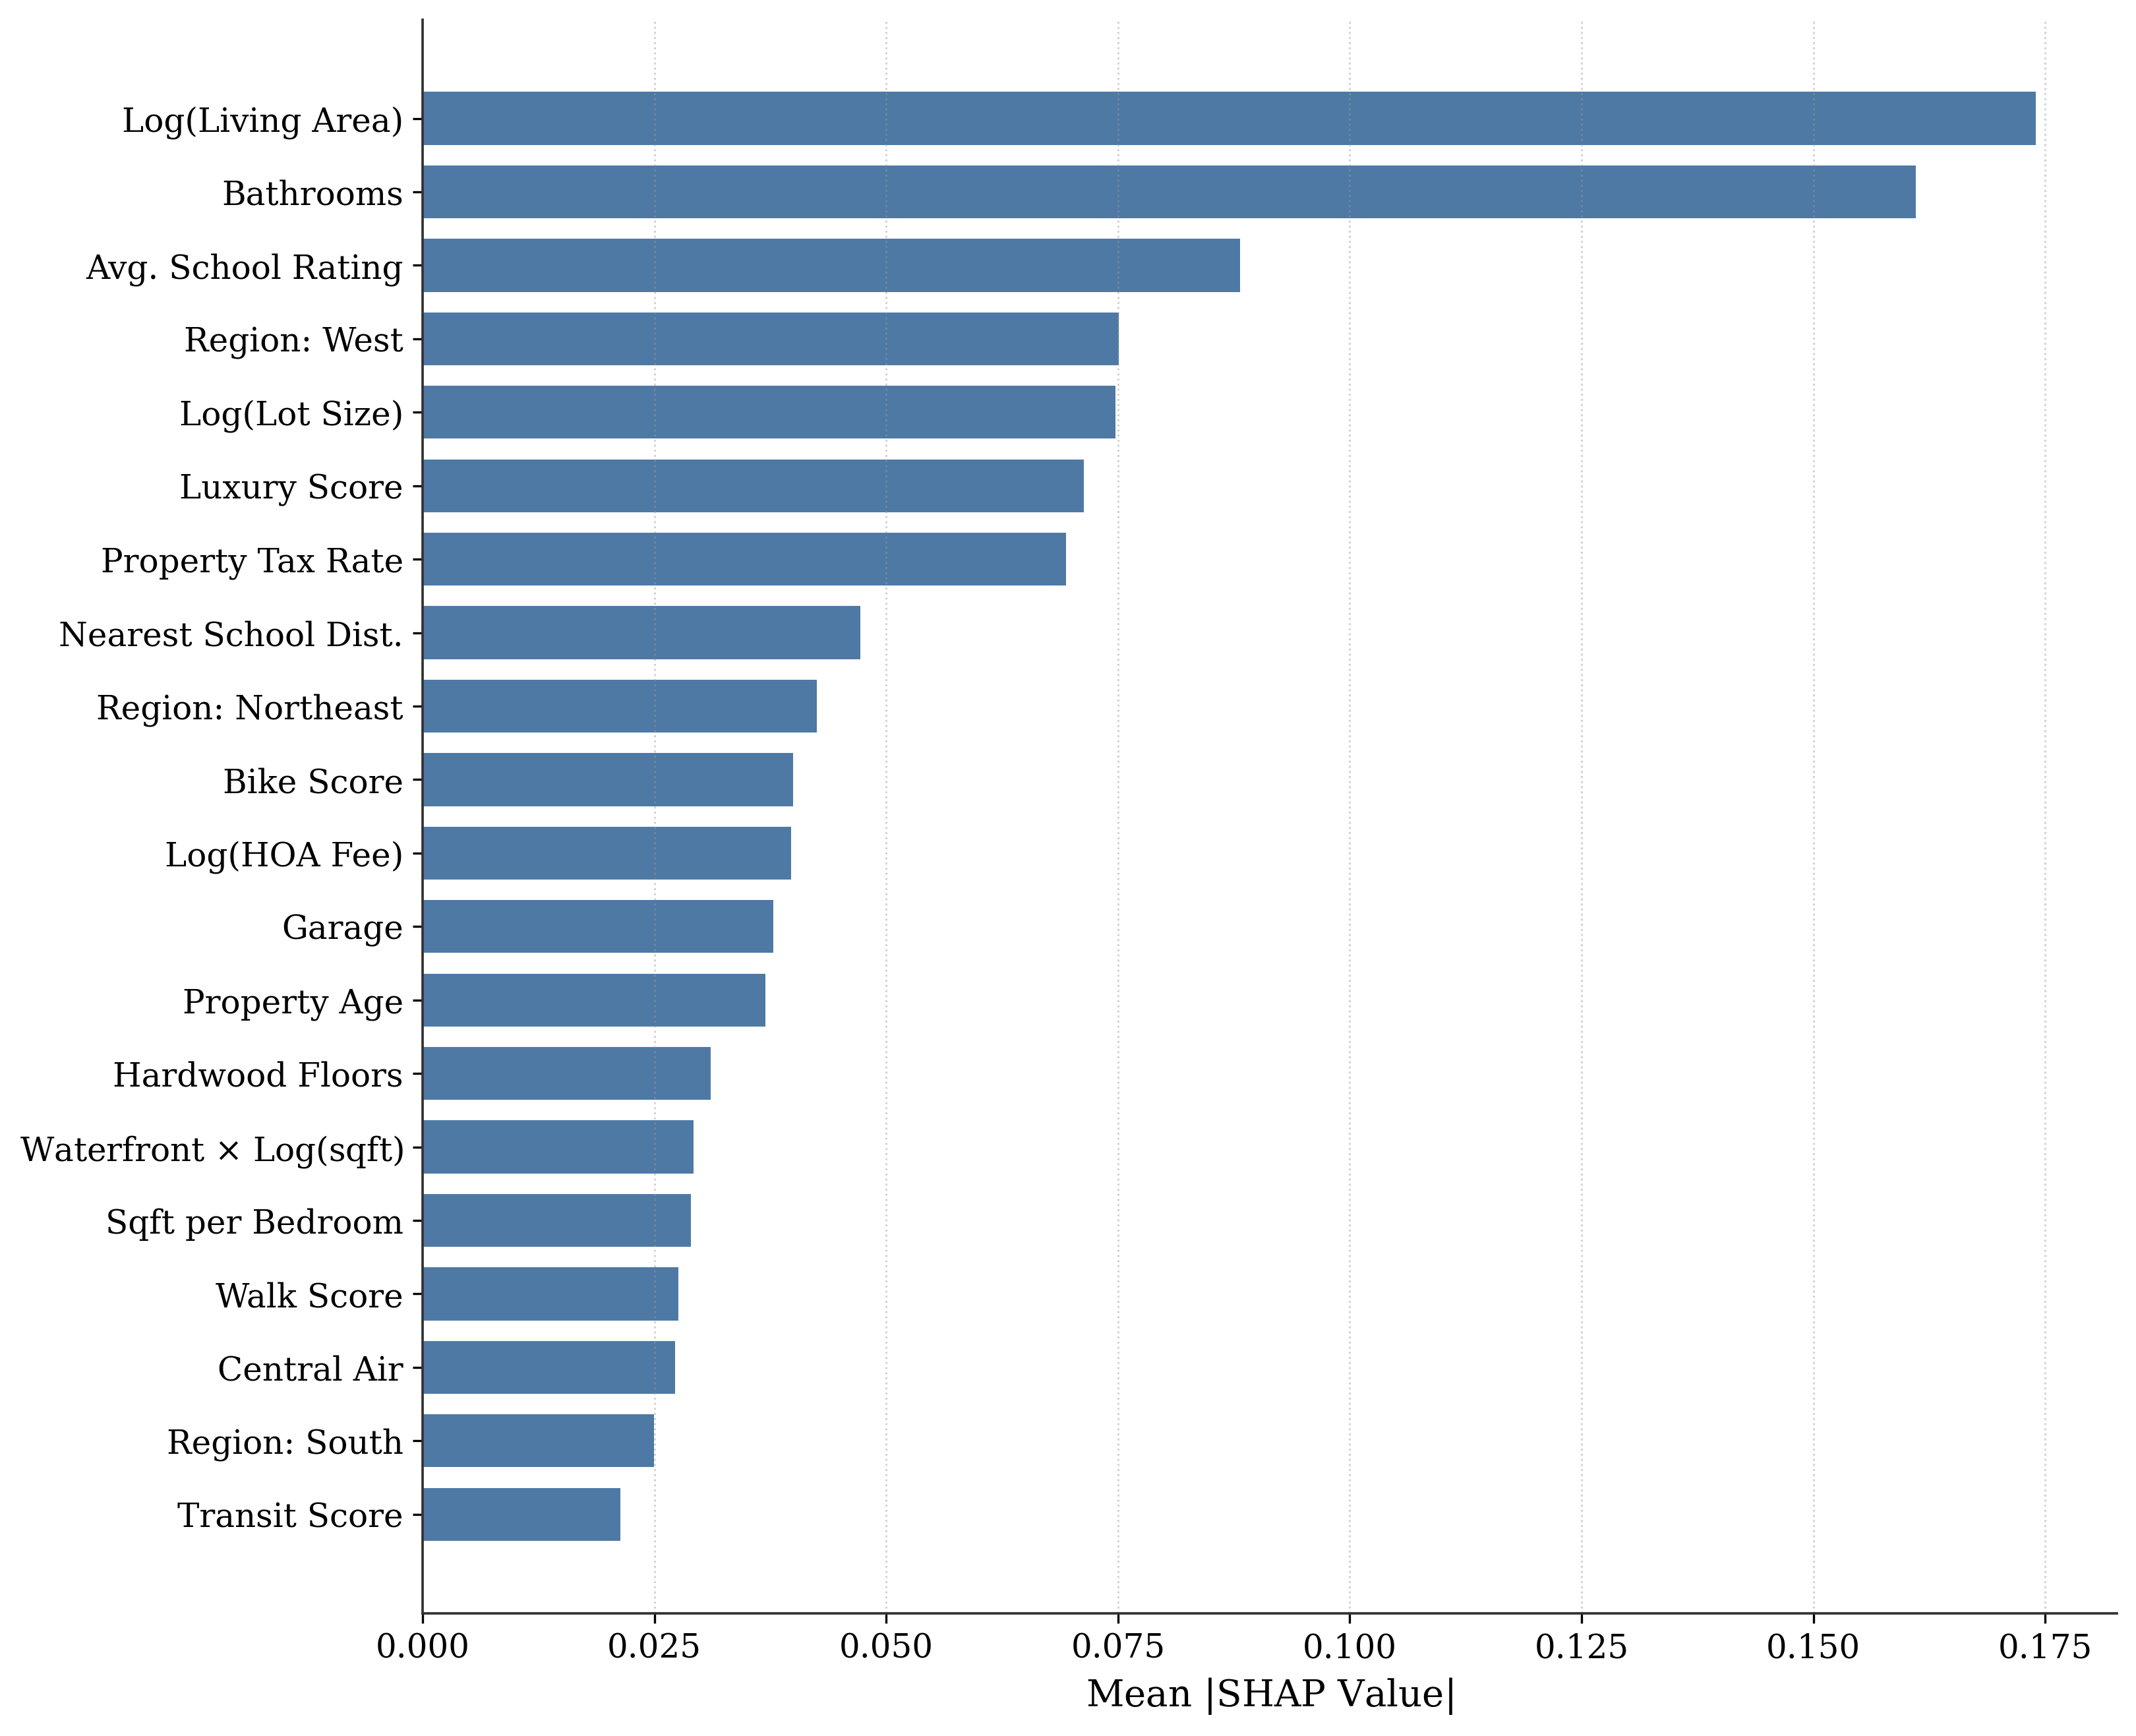
\includegraphics[width=0.85\textwidth]{figures/fig6_shap_importance.png}
    \caption{Feature Importance Bar Chart: Mean Absolute SHAP Values (XGBoost). These values reflect predictive contributions, not causal importance.}
    \label{fig:shap_bar}
\end{figure}

\begin{figure}[H]
    \centering
    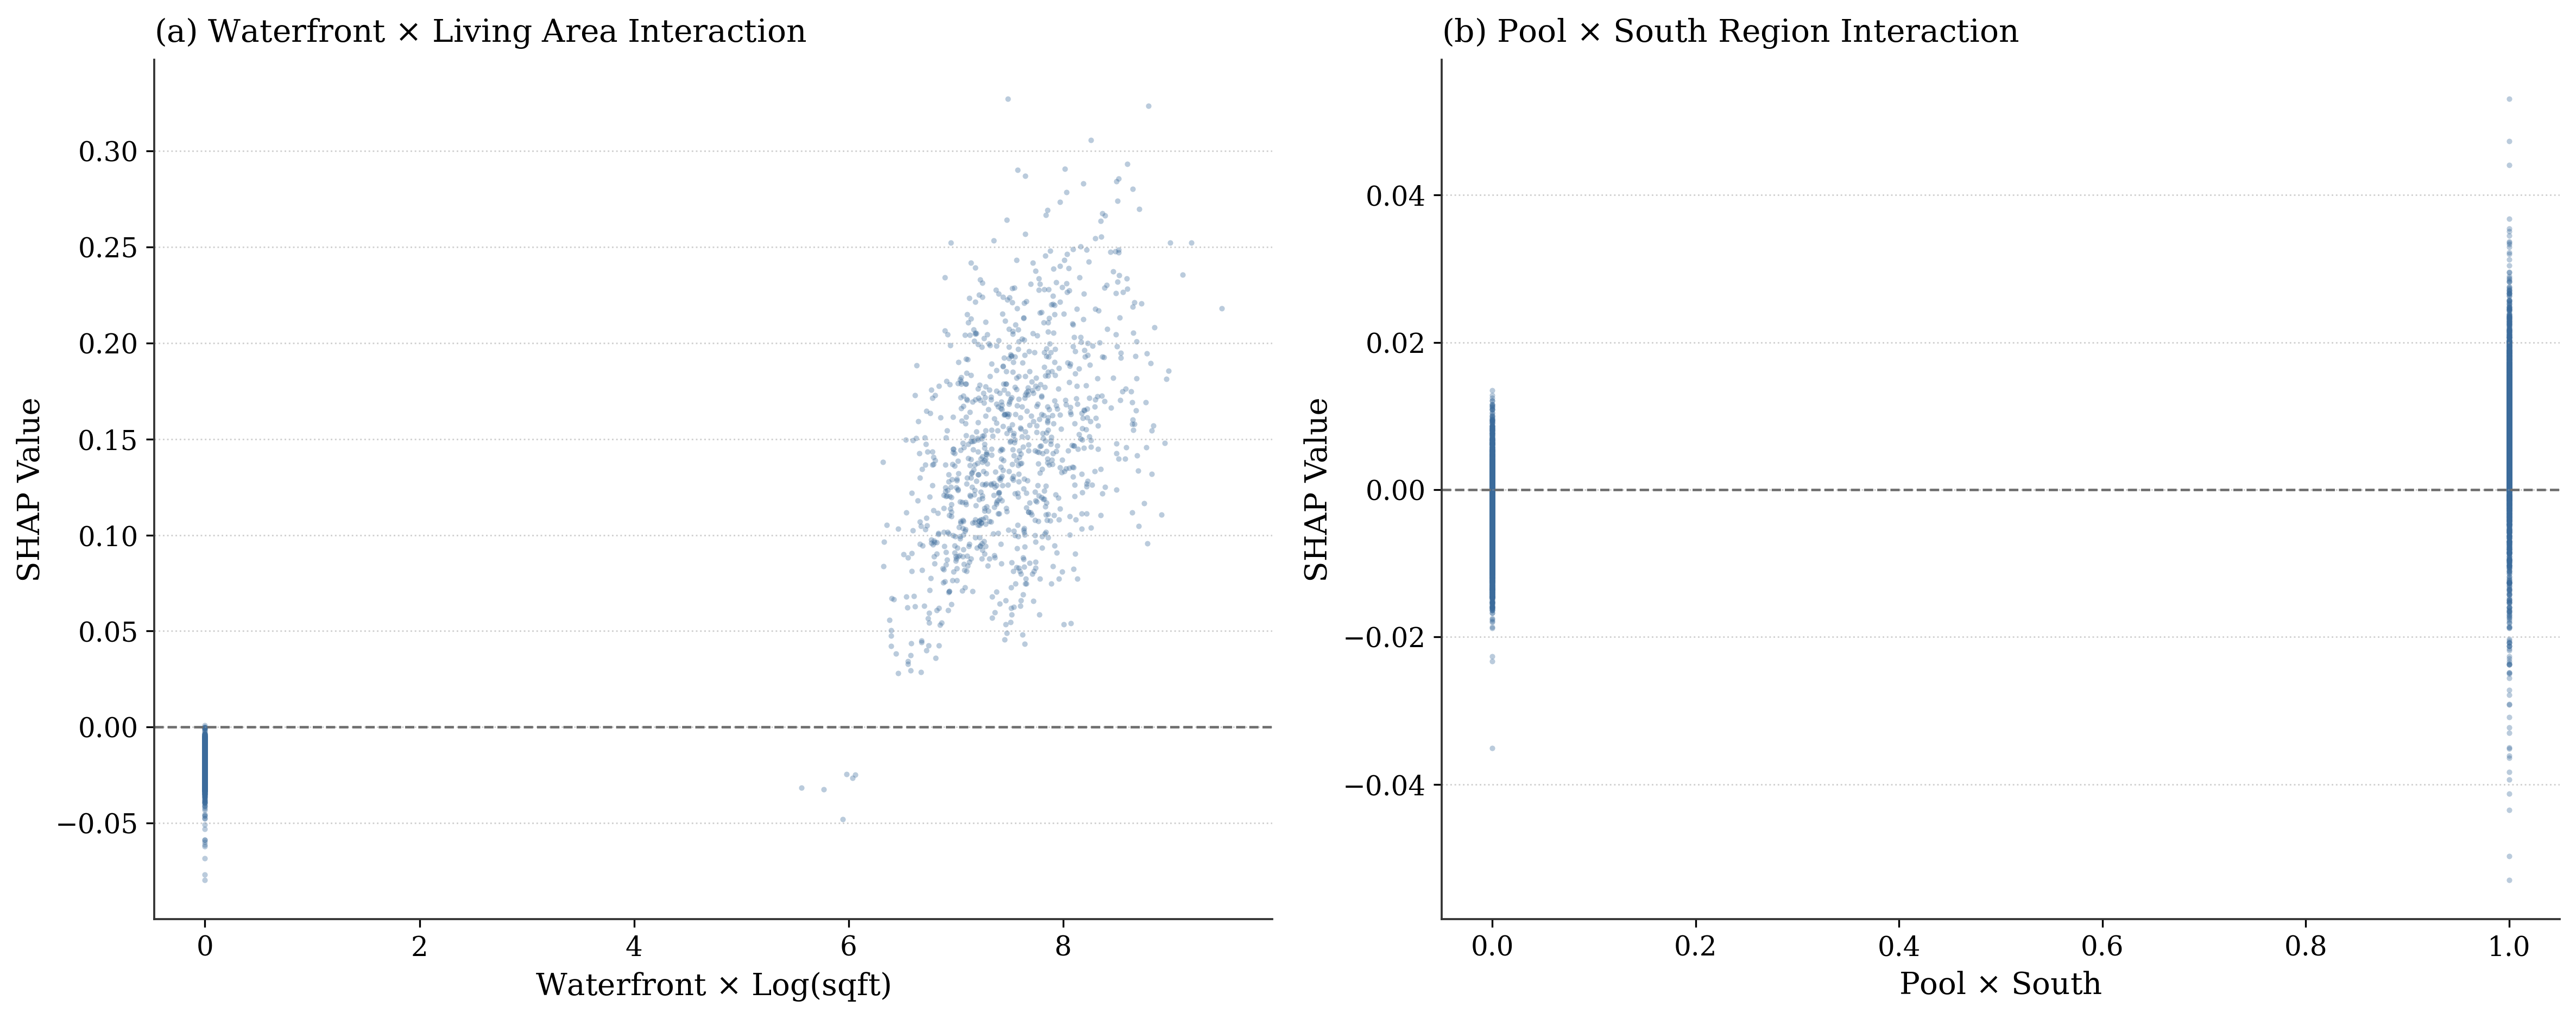
\includegraphics[width=\textwidth]{figures/fig11_shap_interactions.png}
    \caption{SHAP Values for Interaction Terms: (a) Waterfront $\times$ Log(Living Area); (b) Pool $\times$ South Region}
    \label{fig:shap_interactions}
\end{figure}


\section{Full OLS Coefficient Table}
\label{app:ols_full}

Table~\ref{tab:ols_full} reports the complete set of standardized OLS coefficients, including all categorical controls.

\begin{landscape}
\begin{table}[H]
\centering
\caption{Full OLS Regression Results Including All Categorical Controls (Standardized)}
\label{tab:ols_full}
\begin{threeparttable}
\scriptsize
\renewcommand{\arraystretch}{0.9}
\begin{tabular}{lrrlclrrl}
\toprule
Variable & Coeff. & SE & Sig. & & Variable & Coeff. & SE & Sig. \\
\midrule
Constant & 12.510 & 0.010 & *** & & Roof: Metal & 0.070 & 0.008 & *** \\
$\ln$(Living Area)$^\dagger$ & 0.312 & 0.003 & *** & & Roof: Shingle/Comp & $-$0.074 & 0.008 & *** \\
Bedrooms$^\dagger$ & $-$0.068 & 0.002 & *** & & Roof: Tile & $-$0.110 & 0.008 & *** \\
Bathrooms$^\dagger$ & 0.236 & 0.003 & *** & & Roof: Slate & 0.008 & 0.017 & \\
Age$^\dagger$ & $-$0.042 & 0.014 & ** & & Roof: Other & 0.033 & 0.008 & *** \\
Age$^{2\dagger}$ & 0.051 & 0.002 & *** & & Roof: Unknown & 0.004 & 0.008 & \\
Stories$^\dagger$ & 0.000 & 0.000 & & & Constr: Concrete/Block & 0.269 & 0.003 & *** \\
Bath/Bed Ratio$^\dagger$ & $-$0.021 & 0.002 & *** & & Constr: Stucco & 0.149 & 0.002 & *** \\
Sqft/Bed$^\dagger$ & $-$0.002 & 0.002 & & & Constr: Stone & 0.145 & 0.005 & *** \\
$\ln$(Lot Size)$^\dagger$ & 0.070 & 0.001 & *** & & Constr: Wood/Frame & 0.103 & 0.002 & *** \\
Pool & 0.029 & 0.003 & *** & & Constr: Vinyl & 0.012 & 0.002 & *** \\
Spa & 0.033 & 0.003 & *** & & Constr: Steel & 0.027 & 0.014 & * \\
Basement & $-$0.042 & 0.002 & *** & & Constr: Other & 0.075 & 0.002 & *** \\
Fireplace & $-$0.002 & 0.002 & & & Constr: Unknown & 0.177 & 0.002 & *** \\
Garage & 0.109 & 0.002 & *** & & Found: Concrete & 0.217 & 0.005 & *** \\
Waterfront & $-$0.135 & 0.032 & *** & & Found: Crawlspace & 0.181 & 0.006 & *** \\
Central Air & 0.069 & 0.001 & *** & & Found: Slab & 0.122 & 0.005 & *** \\
Forced Air & $-$0.023 & 0.002 & *** & & Found: Pier/Raised & 0.161 & 0.006 & *** \\
Hardwood & 0.125 & 0.001 & *** & & Found: Stone & 0.032 & 0.010 & ** \\
Parking$^\dagger$ & 0.000 & 0.099 & & & Found: Other & 0.144 & 0.006 & *** \\
Luxury$^\dagger$ & 0.044 & 0.002 & *** & & Found: Unknown & 0.174 & 0.005 & *** \\
Walk$^\dagger$ & $-$0.011 & 0.001 & *** & & Northeast & 0.487 & 0.003 & *** \\
Bike$^\dagger$ & 0.072 & 0.001 & *** & & South & 0.022 & 0.003 & *** \\
Transit$^\dagger$ & 0.052 & 0.001 & *** & & West & 0.401 & 0.003 & *** \\
School Rating$^\dagger$ & $-$0.049 & 0.001 & *** & & sqft$\times$Age$^\dagger$ & $-$0.110 & 0.014 & *** \\
School Count$^\dagger$ & $-$0.002 & 0.001 & *** & & Pool$\times$South & 0.008 & 0.001 & *** \\
School Dist.$^\dagger$ & $-$0.016 & 0.001 & *** & & WF$\times$sqft$^\dagger$ & 0.137 & 0.009 & *** \\
Tax Rate$^\dagger$ & $-$0.029 & 0.001 & *** & & Base$\times$North & $-$0.025 & 0.001 & *** \\
Condo & $-$0.037 & 0.004 & *** & & Condo$\times$Walk$^\dagger$ & 0.082 & 0.001 & *** \\
HOA & $-$0.108 & 0.002 & *** & & Age$\times$Lux$^\dagger$ & 0.044 & 0.001 & *** \\
$\ln$(HOA+1)$^\dagger$ & 0.044 & 0.001 & *** & & & & & \\
New Constr. & 0.103 & 0.003 & *** & & & & & \\
Foreclosure & $-$0.406 & 0.010 & *** & & & & & \\
\midrule
\multicolumn{9}{l}{$R^2 = 0.634$, Adj.\ $R^2 = 0.634$, $N = 788{,}842$, $F = 18{,}712.5$, RMSE $= 0.489$} \\
\bottomrule
\end{tabular}
\begin{tablenotes}
\footnotesize
\item \textit{Notes:} HC3 robust standard errors. $^\dagger$Standardized continuous variables. Reference categories: Roof = Flat; Construction = Brick; Foundation = Basement; Region = Midwest. *** $p<0.001$, ** $p<0.01$, * $p<0.05$.
\end{tablenotes}
\end{threeparttable}
\end{table}
\end{landscape}


\section{Robustness Agenda}
\label{app:robustness_agenda}

The following robustness checks and extensions are planned or completed. Items marked with $\checkmark$ have been completed in this version; unmarked items are left for future work.

\begin{enumerate}[nosep]
    \item[$\checkmark$] ZIP3-level fixed effects (Section~\ref{sec:progressive_fe}).
    \item County-level and MSA-level fixed effects.
    \item Spatial lag and spatial error model estimation.
    \item Spatial cross-validation (train on some regions, test on others) at finer geographic levels.
    \item[$\checkmark$] Inter-quantile Wald tests for coefficient equality across quantiles (Section~\ref{sec:qr_results}).
    \item[$\checkmark$] Re-estimation excluding imputed observations (Section~\ref{sec:imputation_sensitivity}).
    \item CatBoost benchmark with native categorical handling.
    \item Nested cross-validation for hyperparameter tuning.
    \item[$\checkmark$] SHAP stability comparison across XGBoost, LightGBM, and Random Forest (Section~\ref{sec:shap_results}).
    \item Integration of climate risk data from First Street Foundation or FEMA flood maps.
    \item Replication using transaction prices from recently sold listings.
    \item GAM/spline models to decompose the ML gain into non-linearity versus spatial partitioning.
    \item Comparison of sample distribution to ACS and Census benchmarks by state and price tier.
    \item Calibration plots by price decile for all models.
    \item[$\checkmark$] Winsorization sensitivity (Section~\ref{sec:winsorization}).
    \item[$\checkmark$] Feature ablation analysis for XGBoost (Section~\ref{sec:ablation}).
    \item[$\checkmark$] XGBoost with latitude/longitude coordinates (Section~\ref{sec:geo_features}).
    \item[$\checkmark$] XGBoost without geographic features (Section~\ref{sec:geo_features}).
    \item[$\checkmark$] Moran's $I$ subsample stability (Section~\ref{sec:spatial_autocorrelation}).
    \item[$\checkmark$] Quantile regression stability across 10 subsamples (Section~\ref{sec:qr_stability}).
\end{enumerate}


\section{Reproducibility Checklist}
\label{app:reproducibility}

\begin{table}[H]
\centering
\caption{Reproducibility Checklist}
\label{tab:reproducibility}
\begin{threeparttable}
\small
\begin{tabular}{p{6cm}p{3cm}p{4cm}}
\toprule
Item & Status & Notes \\
\midrule
\multicolumn{3}{l}{\textit{Data}} \\
Data source identified & Yes & Zillow active listings \\
Sample construction documented & Yes & Table~\ref{tab:attrition} \\
Missing data rates reported & Yes & Table~\ref{tab:missing} \\
Imputation method documented & Yes & State-level medians \\
Imputation sensitivity tested & Yes & Table~\ref{tab:imputation} \\
\midrule
\multicolumn{3}{l}{\textit{Methodology}} \\
Model specifications documented & Yes & Eq.~\ref{eq:ols}--\ref{eq:moran} \\
Hyperparameters reported & Yes & Section~\ref{sec:methodology} \\
Random seeds reported & Yes & Seed = 42 \\
Validation design documented & Yes & Section~\ref{sec:validation_designs} \\
\midrule
\multicolumn{3}{l}{\textit{Results}} \\
Point estimates reported & Yes & Tables~\ref{tab:ols_results}--\ref{tab:shap_stability} \\
Standard errors / CIs reported & Yes (OLS, QR) & HC3 standard errors \\
Multiple comparisons addressed & Partially & Inter-quantile tests \\
Effect sizes in natural units & Yes & Table~\ref{tab:ols_unstd} \\
\midrule
\multicolumn{3}{l}{\textit{Robustness}} \\
Sensitivity to data quality & Yes & Sections~\ref{sec:imputation_sensitivity}--\ref{sec:winsorization} \\
Sensitivity to model choice & Yes & Table~\ref{tab:ml_comparison} \\
Sensitivity to validation design & Yes & Tables~\ref{tab:geo_holdout}--\ref{tab:geo_role} \\
Cross-model stability & Yes & Table~\ref{tab:shap_stability} \\
\midrule
\multicolumn{3}{l}{\textit{Code and Data Availability}} \\
Code available & Yes & Replication package (\texttt{src/}, \texttt{scripts/}, pinned \texttt{requirements.txt}) \\
Data available & On request & Subject to Zillow ToS \\
\bottomrule
\end{tabular}
\begin{tablenotes}
\small
\item \textit{Notes:} This checklist follows recommended practices for empirical reproducibility in applied economics.
\end{tablenotes}
\end{threeparttable}
\end{table}


\end{document}
